% Generated by Sphinx.
\def\sphinxdocclass{report}
\documentclass[letterpaper,10pt,english]{sphinxmanual}
\usepackage[utf8]{inputenc}
\DeclareUnicodeCharacter{00A0}{\nobreakspace}
\usepackage[T1]{fontenc}
\usepackage{babel}
\usepackage{times}
\usepackage[Bjarne]{fncychap}
\usepackage{longtable}
\usepackage{sphinx}


\title{SETLyze Documentation}
\date{December 17, 2010}
\release{1.0}
\author{GiMaRIS}
\newcommand{\sphinxlogo}{}
\renewcommand{\releasename}{Release}
\makeindex

\makeatletter
\def\PYG@reset{\let\PYG@it=\relax \let\PYG@bf=\relax%
    \let\PYG@ul=\relax \let\PYG@tc=\relax%
    \let\PYG@bc=\relax \let\PYG@ff=\relax}
\def\PYG@tok#1{\csname PYG@tok@#1\endcsname}
\def\PYG@toks#1+{\ifx\relax#1\empty\else%
    \PYG@tok{#1}\expandafter\PYG@toks\fi}
\def\PYG@do#1{\PYG@bc{\PYG@tc{\PYG@ul{%
    \PYG@it{\PYG@bf{\PYG@ff{#1}}}}}}}
\def\PYG#1#2{\PYG@reset\PYG@toks#1+\relax+\PYG@do{#2}}

\def\PYG@tok@gd{\def\PYG@tc##1{\textcolor[rgb]{0.63,0.00,0.00}{##1}}}
\def\PYG@tok@gu{\let\PYG@bf=\textbf\def\PYG@tc##1{\textcolor[rgb]{0.50,0.00,0.50}{##1}}}
\def\PYG@tok@gt{\def\PYG@tc##1{\textcolor[rgb]{0.00,0.25,0.82}{##1}}}
\def\PYG@tok@gs{\let\PYG@bf=\textbf}
\def\PYG@tok@gr{\def\PYG@tc##1{\textcolor[rgb]{1.00,0.00,0.00}{##1}}}
\def\PYG@tok@cm{\let\PYG@it=\textit\def\PYG@tc##1{\textcolor[rgb]{0.25,0.50,0.56}{##1}}}
\def\PYG@tok@vg{\def\PYG@tc##1{\textcolor[rgb]{0.73,0.38,0.84}{##1}}}
\def\PYG@tok@m{\def\PYG@tc##1{\textcolor[rgb]{0.13,0.50,0.31}{##1}}}
\def\PYG@tok@mh{\def\PYG@tc##1{\textcolor[rgb]{0.13,0.50,0.31}{##1}}}
\def\PYG@tok@cs{\def\PYG@tc##1{\textcolor[rgb]{0.25,0.50,0.56}{##1}}\def\PYG@bc##1{\colorbox[rgb]{1.00,0.94,0.94}{##1}}}
\def\PYG@tok@ge{\let\PYG@it=\textit}
\def\PYG@tok@vc{\def\PYG@tc##1{\textcolor[rgb]{0.73,0.38,0.84}{##1}}}
\def\PYG@tok@il{\def\PYG@tc##1{\textcolor[rgb]{0.13,0.50,0.31}{##1}}}
\def\PYG@tok@go{\def\PYG@tc##1{\textcolor[rgb]{0.19,0.19,0.19}{##1}}}
\def\PYG@tok@cp{\def\PYG@tc##1{\textcolor[rgb]{0.00,0.44,0.13}{##1}}}
\def\PYG@tok@gi{\def\PYG@tc##1{\textcolor[rgb]{0.00,0.63,0.00}{##1}}}
\def\PYG@tok@gh{\let\PYG@bf=\textbf\def\PYG@tc##1{\textcolor[rgb]{0.00,0.00,0.50}{##1}}}
\def\PYG@tok@ni{\let\PYG@bf=\textbf\def\PYG@tc##1{\textcolor[rgb]{0.84,0.33,0.22}{##1}}}
\def\PYG@tok@nl{\let\PYG@bf=\textbf\def\PYG@tc##1{\textcolor[rgb]{0.00,0.13,0.44}{##1}}}
\def\PYG@tok@nn{\let\PYG@bf=\textbf\def\PYG@tc##1{\textcolor[rgb]{0.05,0.52,0.71}{##1}}}
\def\PYG@tok@no{\def\PYG@tc##1{\textcolor[rgb]{0.38,0.68,0.84}{##1}}}
\def\PYG@tok@na{\def\PYG@tc##1{\textcolor[rgb]{0.25,0.44,0.63}{##1}}}
\def\PYG@tok@nb{\def\PYG@tc##1{\textcolor[rgb]{0.00,0.44,0.13}{##1}}}
\def\PYG@tok@nc{\let\PYG@bf=\textbf\def\PYG@tc##1{\textcolor[rgb]{0.05,0.52,0.71}{##1}}}
\def\PYG@tok@nd{\let\PYG@bf=\textbf\def\PYG@tc##1{\textcolor[rgb]{0.33,0.33,0.33}{##1}}}
\def\PYG@tok@ne{\def\PYG@tc##1{\textcolor[rgb]{0.00,0.44,0.13}{##1}}}
\def\PYG@tok@nf{\def\PYG@tc##1{\textcolor[rgb]{0.02,0.16,0.49}{##1}}}
\def\PYG@tok@si{\let\PYG@it=\textit\def\PYG@tc##1{\textcolor[rgb]{0.44,0.63,0.82}{##1}}}
\def\PYG@tok@s2{\def\PYG@tc##1{\textcolor[rgb]{0.25,0.44,0.63}{##1}}}
\def\PYG@tok@vi{\def\PYG@tc##1{\textcolor[rgb]{0.73,0.38,0.84}{##1}}}
\def\PYG@tok@nt{\let\PYG@bf=\textbf\def\PYG@tc##1{\textcolor[rgb]{0.02,0.16,0.45}{##1}}}
\def\PYG@tok@nv{\def\PYG@tc##1{\textcolor[rgb]{0.73,0.38,0.84}{##1}}}
\def\PYG@tok@s1{\def\PYG@tc##1{\textcolor[rgb]{0.25,0.44,0.63}{##1}}}
\def\PYG@tok@gp{\let\PYG@bf=\textbf\def\PYG@tc##1{\textcolor[rgb]{0.78,0.36,0.04}{##1}}}
\def\PYG@tok@sh{\def\PYG@tc##1{\textcolor[rgb]{0.25,0.44,0.63}{##1}}}
\def\PYG@tok@ow{\let\PYG@bf=\textbf\def\PYG@tc##1{\textcolor[rgb]{0.00,0.44,0.13}{##1}}}
\def\PYG@tok@sx{\def\PYG@tc##1{\textcolor[rgb]{0.78,0.36,0.04}{##1}}}
\def\PYG@tok@bp{\def\PYG@tc##1{\textcolor[rgb]{0.00,0.44,0.13}{##1}}}
\def\PYG@tok@c1{\let\PYG@it=\textit\def\PYG@tc##1{\textcolor[rgb]{0.25,0.50,0.56}{##1}}}
\def\PYG@tok@kc{\let\PYG@bf=\textbf\def\PYG@tc##1{\textcolor[rgb]{0.00,0.44,0.13}{##1}}}
\def\PYG@tok@c{\let\PYG@it=\textit\def\PYG@tc##1{\textcolor[rgb]{0.25,0.50,0.56}{##1}}}
\def\PYG@tok@mf{\def\PYG@tc##1{\textcolor[rgb]{0.13,0.50,0.31}{##1}}}
\def\PYG@tok@err{\def\PYG@bc##1{\fcolorbox[rgb]{1.00,0.00,0.00}{1,1,1}{##1}}}
\def\PYG@tok@kd{\let\PYG@bf=\textbf\def\PYG@tc##1{\textcolor[rgb]{0.00,0.44,0.13}{##1}}}
\def\PYG@tok@ss{\def\PYG@tc##1{\textcolor[rgb]{0.32,0.47,0.09}{##1}}}
\def\PYG@tok@sr{\def\PYG@tc##1{\textcolor[rgb]{0.14,0.33,0.53}{##1}}}
\def\PYG@tok@mo{\def\PYG@tc##1{\textcolor[rgb]{0.13,0.50,0.31}{##1}}}
\def\PYG@tok@mi{\def\PYG@tc##1{\textcolor[rgb]{0.13,0.50,0.31}{##1}}}
\def\PYG@tok@kn{\let\PYG@bf=\textbf\def\PYG@tc##1{\textcolor[rgb]{0.00,0.44,0.13}{##1}}}
\def\PYG@tok@o{\def\PYG@tc##1{\textcolor[rgb]{0.40,0.40,0.40}{##1}}}
\def\PYG@tok@kr{\let\PYG@bf=\textbf\def\PYG@tc##1{\textcolor[rgb]{0.00,0.44,0.13}{##1}}}
\def\PYG@tok@s{\def\PYG@tc##1{\textcolor[rgb]{0.25,0.44,0.63}{##1}}}
\def\PYG@tok@kp{\def\PYG@tc##1{\textcolor[rgb]{0.00,0.44,0.13}{##1}}}
\def\PYG@tok@w{\def\PYG@tc##1{\textcolor[rgb]{0.73,0.73,0.73}{##1}}}
\def\PYG@tok@kt{\def\PYG@tc##1{\textcolor[rgb]{0.56,0.13,0.00}{##1}}}
\def\PYG@tok@sc{\def\PYG@tc##1{\textcolor[rgb]{0.25,0.44,0.63}{##1}}}
\def\PYG@tok@sb{\def\PYG@tc##1{\textcolor[rgb]{0.25,0.44,0.63}{##1}}}
\def\PYG@tok@k{\let\PYG@bf=\textbf\def\PYG@tc##1{\textcolor[rgb]{0.00,0.44,0.13}{##1}}}
\def\PYG@tok@se{\let\PYG@bf=\textbf\def\PYG@tc##1{\textcolor[rgb]{0.25,0.44,0.63}{##1}}}
\def\PYG@tok@sd{\let\PYG@it=\textit\def\PYG@tc##1{\textcolor[rgb]{0.25,0.44,0.63}{##1}}}

\def\PYGZbs{\char`\\}
\def\PYGZus{\char`\_}
\def\PYGZob{\char`\{}
\def\PYGZcb{\char`\}}
\def\PYGZca{\char`\^}
% for compatibility with earlier versions
\def\PYGZat{@}
\def\PYGZlb{[}
\def\PYGZrb{]}
\makeatother

\begin{document}

\maketitle
\tableofcontents
\phantomsection\label{index::doc}



\chapter{About SETLyze}
\label{index:welcome-to-setlyze-s-documentation}\label{index:about-setlyze}
The purpose of SETLyze is to provide the people involved with the SETL
project (mostly biologists) an easy and fast way of getting useful information from
the data stored in the SETL database. The database was created so certain
analysis could be done which would provide more insight in a set of
biological questions. The application should be capable of giving answer
to those questions by applying specific analysis to the data and
providing the user with an understandable overview of the results.

SETLyze is be capable of performing the following analysis:
\begin{description}
\item[{\emph{Analysis 1 ``Spot Preference''}}] \leavevmode
Determine a species’ preference for a specific location on a SETL
plate.

\item[{\emph{Analysis 2.1 ``Attraction of Species (intra-specific)''}}] \leavevmode
Determine if a specie attracts or repels individuals of its own kind.

\item[{\emph{Analysis 2.2 ``Attraction of Species (inter-specific)''}}] \leavevmode
Determine if two different species attract or repel each other.

\end{description}

The following analysis have not been implemented yet:
\begin{description}
\item[{\emph{Analysis 3 ``Relation between Species''}}] \leavevmode
Determine if there is a relation between two (groups of) species on
SETL plates in a location. Plates per location are compared. And
instead of looking at different plate spots, only the presence or
absence of a specie on a plate is taken into account.

\end{description}


\chapter{Documentations}
\label{index:documentations}

\section{SETLyze User Manual}
\label{user_manual::doc}\label{user_manual:setlyze-user-manual}
Welcome to the user manual for SETLyze. This manual is intended for the
end user and explains how to use SETLyze.


\subsection{Introduction to SETLyze}
\label{user_manual:introduction-to-setlyze}
SETLyze is a part of the \href{http://www.anemoon.org/setl/}{SETL-project},
a fouling community study focussing on marine invasive species. This
project is being lead by Arjan Gittenberger. The website describes the
SETL-project as follows:
\begin{quote}

``Over the last ten years, marine invaders have had a dramatically
increasing impact on temperate water ecosystems around the world.
Substantial ecological and economical damage has been caused by the
introduction of diseases, parasites, predators, invaders outcompeting
native species, and species that are a nuisance for public health,
tourism, aquaculture or in any other way. In the SETL-project
standardized PVC-plates are used to detect these invasive species
and other fouling community organisms. The material and methods of
the SETL-project were developed by the ANEMOON foundation in
cooperation with the Smithsonian Marine Invasions Laboratory of
Smithsonian Environmental Research Centre. In this project 14x14
cm PVC-plates are hung 1 meter below the water surface, and refreshed
and checked for species at least every three months.'' ---
\href{http://www.anemoon.org/setl/}{ANEMOON foundation - SETL}
\end{quote}

Data collected from these SETL plates are being collected in
the SETL database. This database contains over 25000 records containing
information of over 200 species in different localities throughout the
Netherlands. SETLyze is an application which is capable of performing
a set of analysis on the data from the SETL database. SETLyze is
be capable of performing the following analysis:
\begin{description}
\item[{\emph{Analysis 1 ``Spot Preference''}}] \leavevmode
Determine a species’ preference for a specific location on a SETL
plate.

\item[{\emph{Analysis 2.1 ``Attraction of Species (intra-specific)''}}] \leavevmode
Determine if a specie attracts or repels individuals of its own kind.

\item[{\emph{Analysis 2.2 ``Attraction of Species (inter-specific)''}}] \leavevmode
Determine if two different species attract or repel each other.

\end{description}

The following analysis have not been implemented yet:
\begin{description}
\item[{\emph{Analysis 3 ``Relation between Species''}}] \leavevmode
Determine if there is a relation between two (groups of) species on
SETL plates in a location. Plates per location are compared. And
instead of looking at different plate spots, only the presence or
absence of a specie on a plate is taken into account.

\end{description}


\subsubsection{Data Collection}
\label{user_manual:data-collection}
First let's have a look at how the data for the SETL-project is being
collected. When the SETL plates are checked, each plate is first
carefully pulled out of the water and then photographed. All this is
done following a standard procedure described on the ANEMOON
foundation's website. First an overview photograph is taken of each
plate. Then some more detailed photographs are taken of the species
that grow on each plate. Indivdual plates are recognized by their tags.
The pictures are then carefully analyzed. For each plate the
SETL-monitoring form is filled in. For each species the absence or
presence, abundance and area cover are filled in. For this, a 5x5 grid
is digitally applied over the photograph. For each specie the presence
or absence on each of the 25 plate surfaces are filled in and saved
to the database.
\begin{figure}[htbp]
\centering
\capstart

\scalebox{1.000000}{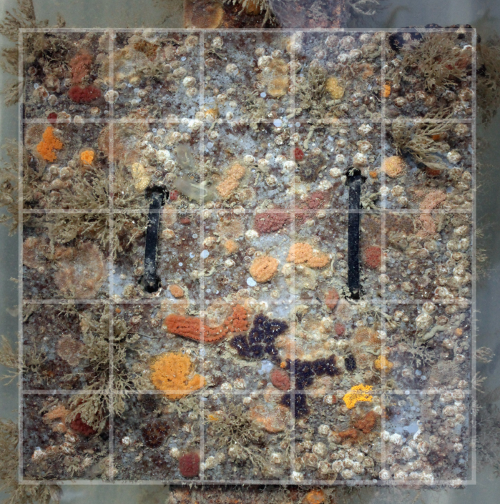
\includegraphics{setl_plate_with_grid.png}}
\caption{Figure 1. SETL-plate with digitally applied grid}\label{user_manual:fig-plate-with-grid}\end{figure}

Each record in the database contains a specie ID, a plate ID, and
the 25 plate surfaces. The specie ID links to the specie that was found
on the plate. The plate ID links to the plate on which that specie was
found. The plate ID is also linked to the location where this plate
was deployed. The 25 plate surfaces (``spots'') are stored in each record
as booleans (meaning they can have a value of True or False). The value
1 (True) for a spot means that the specie in question was present on
that spot of the plate. The value 0 (False) means that the specie
was absent from that spot.

With 25 x 2500 = 625000+ booleans for the presence/absence of species,
automatic methods of analyzing this data are required. Hence SETLyze
was developed, a tool for analyzing the settlement of species
on SETL plates.


\subsubsection{Using SETLyze}
\label{user_manual:using-setlyze}
SETLyze comes with a graphical user interface (GUI). The GUI consists
of dialogs which all have a specific task. These dialogs will guide
you in performing the set of analysis it provides. Most of SETLyze's
dialogs have a Help button. Clicking this Help button should point you
to the corresponding dialog description on this page. All dialog
descriptions can be found in the {\hyperref[user_manual:setlyze-dialogs]{\emph{SETLyze dialogs}}}
section of this manual.

Before SETLyze can perform an analysis, it needs access to a data
source containing SETL data. Currently just one data source is
supported: manually exported CSV files from the Microsoft Access SETL
database. This means that the user must first export the tables of the
SETL database from Microsoft Access to CSV files. This would result in
four CSV files, one for each table. The user is then required to load
these files into SETLyze. First follow {\hyperref[user_manual:export-csv-msaccess]{\emph{the steps to export the
SETL data to CSV files}}}.

You can perform an analysis once you have the four CSV files containing
the SETL data. First run SETLyze by (double) clicking the file named
\code{setlyze.pyw}. You should be presented with the
{\hyperref[user_manual:dialog-analysis-selection]{\emph{analysis selection dialog}}}. Select
the analysis you want to perform and press OK to begin. A new dialog
will be displayed, most likely the
{\hyperref[user_manual:dialog-loc-selection]{\emph{locations selection dialog}}}.

If this is your first time running SETLyze, the locations selection
dialog will show an empty locations list. The list is empty because the
data source has not been set yet. To set the data source and load the
SETL data, click on the \emph{Change Data Source} button to open the
{\hyperref[user_manual:dialog-change-data-source]{\emph{change data source dialog}}}. This
dialog allows you to load the data from the CSV files you've just
created.

Once the data has been loaded, the locations selection dialog will
automatically update the list of locations. From here on it's just a
matter of following the instruction one the dialogs. Should you need
more help, scroll down to the {\hyperref[user_manual:setlyze-dialogs]{\emph{SETLyze dialogs}}}
section for a more extensive description of each dialog. The dialog
descriptions are also accessible from SETLyze's dialogs itself by
clicking the Help button on a dialog.


\subsection{Definition List}
\label{user_manual:definition-list}
This part of the user manual describes some terminology often used
throughout the application and this manual.
\begin{description}
\item[{Spot}] \leavevmode
To analyze SETL plates, photographs of the plates are taken. The
photographs are then analyzed on the computer by applying a 5x5
grid to the photographs. This divides the SETL plate into 25 equal
surface areas (see {\hyperref[user_manual:fig-plate-with-grid]{\emph{figure 1}}}). Each
of the 25 surface areas are called ``spots''. Species are scored for
presence/absence for each of the 25 spots on each SETL plate, and the
data is stored in the SETL database in the form of records. So each
SETL record in the database contains presence/absence data of one
specie for all 25 spots on a SETL plate.

\item[{Positive spot}] \leavevmode
Each record in the SETL database contains data for each of the 25
spots on a SETL plate. The spots are stored as booleans, meaning
they can have two values; 1 (True) means that the specie was present
on that spot, 0 (False) means that the species was absent on
that spot. A spot is ``positive'' if the spot value is 1 or True. Each
record can thus have up to 25 positive spots.

\end{description}


\subsection{SETLyze dialogs}
\label{user_manual:setlyze-dialogs}\label{user_manual:id1}
SETLyze comes with a graphical user interface consisting of separate
dialogs. The dialogs are described in this section.


\subsubsection{Analysis Selection dialog}
\label{user_manual:analysis-selection-dialog}\label{user_manual:dialog-analysis-selection}\begin{figure}[htbp]
\centering
\capstart

\scalebox{1.000000}{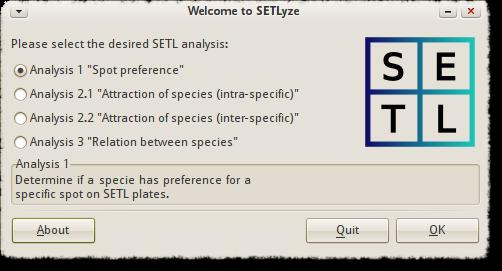
\includegraphics{dialog_select_analysis.jpg}}
\caption{Figure 2. Analysis Selection dialog}\end{figure}

The analysis selection dialog is the first dialog you see when SETLyze
is started. It allows the user to select an analysis to perform on SETL
data. The user can select one of the analysis in the list and click on
the OK button to start the analysis. Clicking the Quit button closes
the application.

After pressing the OK button, two things can happen. If no SETL data was
found on the user's computer, SETLyze automatically tries to load SETL
localities and species data from the remote SETL database. This requires
a direct connection with the SETL database server. A progress dialog is
shown while the data is being loaded.

If SETL data is found on the user's computer, a message dialog is shown
presenting the user with two options. Option one is to use the SETL data
that was previously saved to the user's computer. Option two is to
discard the saved data and load data from the remote SETL database.

Clicking the About button shows SETLyze's About dialog. The About dialog
shows basic information about SETLyze; its version number, license
information, a link to the GiMaRIS website, the application developers,
and contact information.


\subsubsection{Locations Selection dialog}
\label{user_manual:dialog-loc-selection}\label{user_manual:locations-selection-dialog}\begin{figure}[htbp]
\centering
\capstart

\scalebox{1.000000}{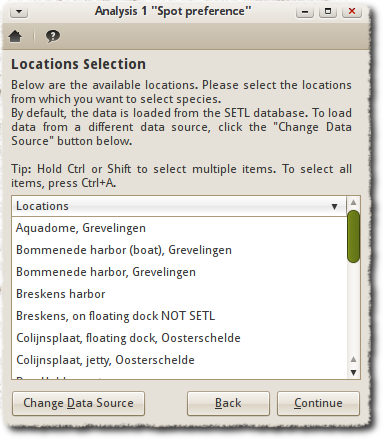
\includegraphics{dialog_locations_selection.png}}
\caption{Figure 3. Locations Selection dialog}\end{figure}

The locations selection dialog shows a list of all SETL localities. This
dialog allows you to select locations from which you want to select
species. The {\hyperref[user_manual:dialog-spe-selection]{\emph{species selection dialog}}}
(displayed after clicking the Continue button) will only display the
species that were recorded in the selected locations. Subsequently this
means that only the SETL records that match both the locations and
species selection will be used for the analysis, as each SETL record
is bound to a specie and a SETL plate from a specific location.

The \emph{Change Data Source} button opens the
{\hyperref[user_manual:dialog-change-data-source]{\emph{change data source dialog}}}. This
dialog allows you to switch to a different data source. After doing so,
the locations selection dialog is automatically updated with the new
data.

The Back button allows you to go back to the previous dialog. This can
be useful when you want to correct a choice you made in a previous
dialog.

The Continue button saves the choices you made in that dialog, closes
the dialog, and shows the next dialog.


\paragraph{Making a selection}
\label{user_manual:making-a-selection}
Just click on one of the locations to select it. To select multiple
locations, hold Ctrl or Shift while selecting. To select all locations
at once, click on a location and press Ctrl+A.


\subsubsection{Species Selection dialog}
\label{user_manual:dialog-spe-selection}\label{user_manual:species-selection-dialog}\begin{figure}[htbp]
\centering
\capstart

\scalebox{1.000000}{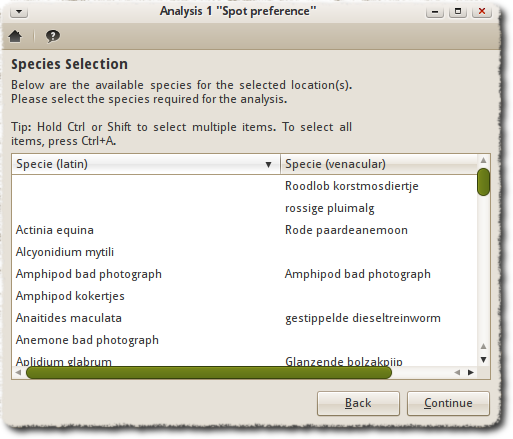
\includegraphics{dialog_species_selection.png}}
\caption{Figure 4. Species Selection dialog}\end{figure}

The species selection dialog shows a list of all SETL species that were
found in the selected SETL localities. This dialog allows you to select
the species to be included in the analysis. Only the SETL records that
match both the the locations and species selection will be used for the
analysis.

It is possible to select more than one specie (see \emph{Making a selection}).
Selecting more than one specie in a single species selection dialog
means that the selected species are threated as one specie for the
analysis. However, if the selected analysis requires two or more
separate specie selections (i.e. two species are compared), it will
display the selection dialog multiple times. In this case, the
header of the selection dialog will say ``First Species Selection'',
``Second Species Selection'', etc.

The Back button allows you to go back to the previous dialog. This can
be useful when you want to correct a choice you made in a previous
dialog.

The Continue button saves the choices you made in that dialog, closes
the dialog, and shows the next dialog.


\paragraph{Making a selection}
\label{user_manual:id2}
Just click on one of the species to select it. To select multiple
species, hold Ctrl or Shift while selecting. To select all species
at once, click on a specie and press Ctrl+A.


\subsubsection{Change Data Source dialog}
\label{user_manual:dialog-change-data-source}\label{user_manual:change-data-source-dialog}\begin{figure}[htbp]
\centering
\capstart

\scalebox{1.000000}{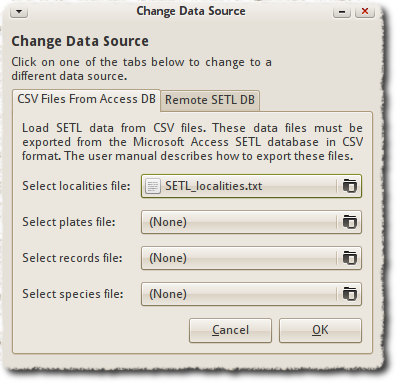
\includegraphics{dialog_change_data_source.png}}
\caption{Figure 5. Change Data Source dialog}\end{figure}

The change data source dialog allows you to switch to a different data
source. Two data sources are possible:
\begin{itemize}
\item {} 
CSV files exported from the Microsoft Access SETL database. The CSV
files need to be exported by Microsoft Access, one file for each of
the four tables: SETL\_localities, SETL\_plates, SETL\_records, and
SETL\_species. The section
{\hyperref[user_manual:export-csv-msaccess]{\emph{Exporting CSV Files from the MS Access database}}}
describes how to export these files.

After selecting all four CSV files, press the OK button to load all
SETL data from these files. A progress dialog is shown while the data
is being loaded. Once the data has been loaded, the
{\hyperref[user_manual:dialog-loc-selection]{\emph{locations selection dialog}}} will be
updated with the new data.

\item {} 
The remote SETL database. The remote SETL database has not been
created yet, so this functionality is not implemented yet. The idea is
to move the data from the Microsoft Access database to a PostgreSQL
database.

This dialog should allow you to enter the information needed to
connect to the remote database (i.e. the server address and a port number),
Pressing the OK button should load the localities and species data.
A progress dialog is shown while the data is being loaded. Once the
data has been loaded, the
{\hyperref[user_manual:dialog-loc-selection]{\emph{locations selection dialog}}} will be
updated with the new data.

The plates and records data will not be loaded directly (in contrast
to loading data from CSV files). The plates and record data will be
loaded when required by the analysis.

\end{itemize}


\subsubsection{Define Plate Areas dialog}
\label{user_manual:define-plate-areas-dialog}\label{user_manual:dialog-define-plate-areas}\begin{figure}[htbp]
\centering
\capstart

\scalebox{1.000000}{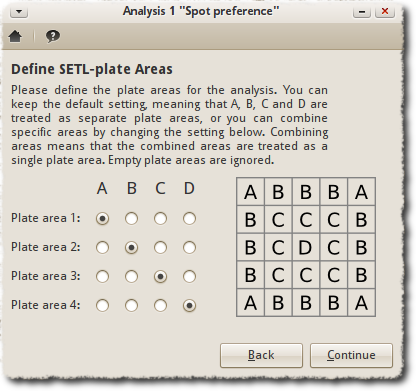
\includegraphics{dialog_define_plate_areas.png}}
\caption{Figure 6. Define Plate Areas dialog}\end{figure}

This dialog allows you to define the plate areas for analysis 1
``spot preference''. By default, the SETL plate is devided in four plate
areas: A, B, C and D. This dialog allows you to combine specific areas by
changing the areas selection in the dialog. Combining areas means that
the combined areas are treated as a single plate area.

Below is a schematic SETL-plate with a grid. By default the plate is
divided in four plate areas (A, B, C and D),
\begin{figure}[htbp]
\centering

\scalebox{1.000000}{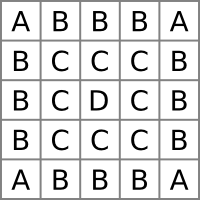
\includegraphics{plate_areas_default.png}}
\end{figure}

But sometimes it's useful to combine plate areas. So if the user decides
to combine area A and B, the areas selection would be set like this,
\begin{figure}[htbp]
\centering

\scalebox{1.000000}{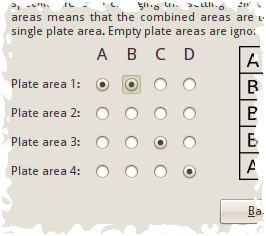
\includegraphics{plate_areas_selection_combined1.png}}
\end{figure}

And the resulting plate areas definition would look something like this,
\begin{figure}[htbp]
\centering

\scalebox{1.000000}{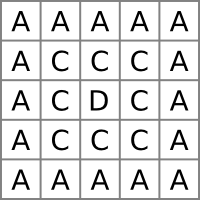
\includegraphics{plate_areas_combined1.png}}
\end{figure}

This would result in three plate areas. Analysis 1 would then determine
if the selected specie has a preference for either of the three plate
areas.

The names of the plate areas (area 1, area 2, ...) do not have a
special meaning. It is simply used internally by the application to
distinguish between plate areas. These area names are also used in the
analysis report to distinguish between the plate areas.

The Back button allows you to go back to the previous dialog. This can
be useful when you want to correct a choice you made in a previous
dialog.

The Continue button saves the choices you made in the dialog, closes
the dialog, and shows the next dialog.


\subsubsection{Analysis Report dialog}
\label{user_manual:analysis-report-dialog}\label{user_manual:dialog-analysis-report}\begin{figure}[htbp]
\centering
\capstart

\scalebox{1.000000}{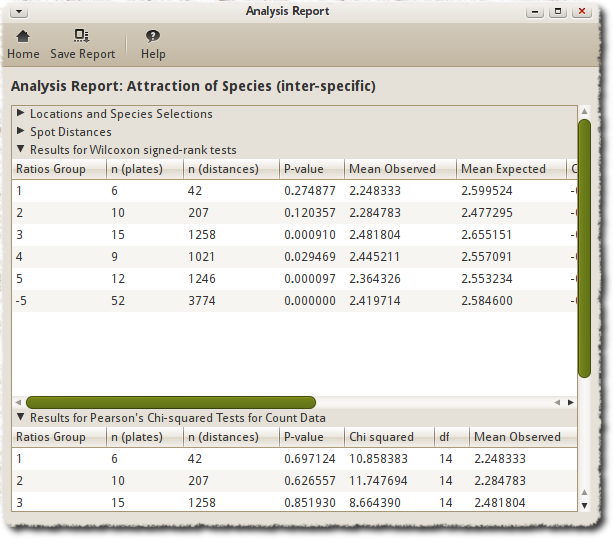
\includegraphics{dialog_analysis_report.png}}
\caption{Figure 10. Analysis Report dialog}\end{figure}

The analysis report dialog shows the results for the anaylysis. The
report is divided into sub sections. Each sub section is described
below.


\paragraph{Locations and Species Selections}
\label{user_manual:locations-and-species-selections}
Displays the locations and species selections. If multiple selections
were made, each element is suffixed by a number. For example ``Species
selection (2)'' stands for the second species selection.


\paragraph{Spot Distances}
\label{user_manual:spot-distances}
Displays the observed and expected spot distances. The observed spot
distances are calculated as follows:
\begin{itemize}
\item {} 
In the case of analysis 2.1, intra-specific: All possible distances
between the spots on each plate are calculated using the Pythagorean
theorem. Consider the case of specie A and the following plate:
\begin{quote}
\begin{figure}[htbp]
\centering

\scalebox{1.000000}{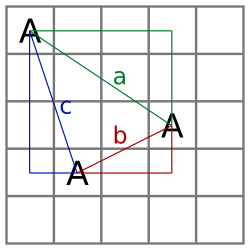
\includegraphics{setl_plate_intra_distances.png}}
\end{figure}
\end{quote}

As you can see from the figure, three positive spots results in three
spot distances (\emph{a}, \emph{b} and \emph{c}). This distance from one spot to the next
by moving horizontally or vertically defined 1. So for example, the
distance for \emph{a} is calculated by applying Pythagoras' theorem on the
green triangle. The distance for \emph{a} would be $\sqrt{3^2 + 2^2} = 3.61$.
This is done for all possible spot distances on each plate. This
results in a list of observed spot distances.

\item {} 
In the case of analysis 2.2 inter-specific: First the plate records
are collected that contain both of the selected species. Then all
possible spot distances are calculated between the two species. The
following figure shows an example with positive spots for two species
(A and B) and all possible spot distnaces.
\begin{quote}
\begin{figure}[htbp]
\centering

\scalebox{1.000000}{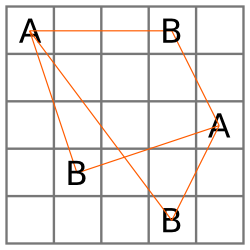
\includegraphics{setl_plate_inter_distances.png}}
\label{user_manual:fig-spot-distances-inter}\end{figure}
\end{quote}

The distances are calculated the same way as for analysis 2.1.

\end{itemize}

The expected spot distances are calculated by generating a copy of
each plate record matching the species selection. Each copy has the
same number of positive spots as its original, except the positive
spots are placed randomly at the plates. Then the spot distances
are calculates the same way as for the observed spot distances. This
mean that the resulting list of expected spot distances has the same
length as the observed spot distances.


\paragraph{Results for Wilcoxon signed-rank test}
\label{user_manual:results-for-wilcoxon-signed-rank-test}
Shows the results for the Wilcoxon signed-rank test.
\begin{quote}

``The Wilcoxon signed-rank test is a non-parametric statistical
hypothesis test for the case of two related samples or repeated
measurements on a single sample. It can be used as an alternative
to the paired Student's t-test when the population cannot be assumed
to be normally distributed.'' ---
\href{http://en.wikipedia.org/wiki/Wilcoxon\_test}{Wikipedia - Wilcoxon signed-rank test}
\end{quote}

Tests showed that spot distances on a SETL plate are not normally
distributed (see {\hyperref[user_manual:fig-distance-distribution-intra]{\emph{figure 13}}}
and {\hyperref[user_manual:fig-distance-distribution-inter]{\emph{14}}}), hence the Wilcoxon
test was chosen to test if the observed and expected spot distances
differ significantly.
\begin{figure}[htbp]
\centering
\capstart

\scalebox{1.000000}{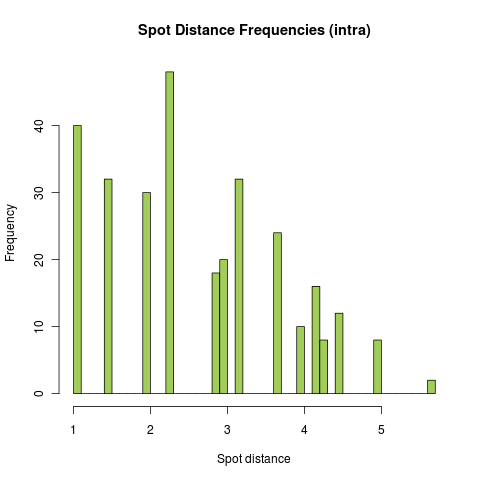
\includegraphics{distance_distribution_intra.png}}
\caption{Figure 13. Distribution for intra-specific spot distances. The
frequencies were obtained by calculating all possible distances
between two spots if all 25 spots are covered.
The same test was done with different numbers of positive spots
randomly placed on a plate with 100.000 repeats. All
resulting distributions are very similar to this figure.}\label{user_manual:fig-distance-distribution-intra}\end{figure}
\begin{figure}[htbp]
\centering
\capstart

\scalebox{1.000000}{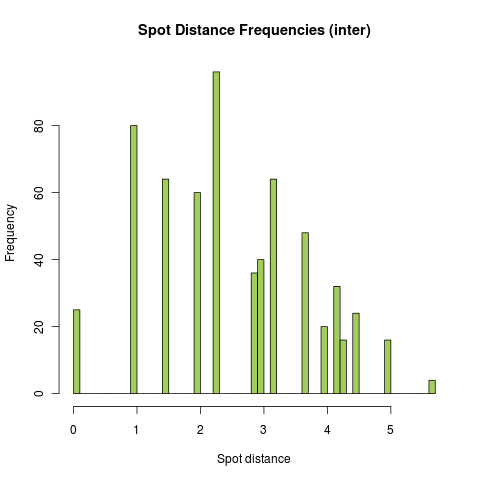
\includegraphics{distance_distribution_inter.png}}
\caption{Figure 14. Distribution for inter-specific spot distances. The
frequencies were obtained by calculating all possible distances
between two spots with ratio 25:25 (specie A and B have all 25 spots
covered). The same test was done with different positive spots
ratios (spots randomly placed on a plate, 100.000 repeats). All
resulting distributions are very similar to this figure.}\label{user_manual:fig-distance-distribution-inter}\end{figure}

Depending on the analysis, the records matching the species selection
are first grouped by positive spots number (analysis 2.1) or by ratios
group (analysis 2.2).
\begin{itemize}
\item {} 
Records grouped by number of positive spots: This results in a
maximum of 25 groups. Group 1 contains records with just 1 positive
spot, group 2 contains records with 2 positive spots, et cetera.
however, group 1 and 25 are skipped. Group 1 is excluded because it
is not possible to calculate spot distances for records with just one
positive spot. Group 25 is excluded because a test on these records
will always result in a p-value of 1. This is because the observed
spot distances will always be the same as the expected distances.
The test is also performed on a group with positive spots number -24.
This actually means ``up to that number of positive spots''. So this
test is also performed on records with up to 24 positive spots. Note
that records with 1 positive spot will still be excluded.

So the test is performed 24 times, and each test result is presented on
a different row. Each row contains the result of the test for a group.

\item {} 
Records grouped by ratios groups: In analysis 2.2 we're dealing with
two species. For this analysis plate records are matched that contain
both species. This means we can get a ratio of positive spots for each
SETL plate.
Consider figure \emph{fig\_spot-distances-inter} which shows positive
spots of species A and B. There are two positive spots of one specie,
and three positive spots of the other. That makes the ratio for this
plate 2:3. The order of the species doesn't matter, so ratio A:B is
considered the same as ratio B:A. All records are grouped based on
this ratio. We've defined five ratios groups:

\begin{notice}{note}{Note:}\begin{description}
\item[{\emph{comb()}}] \leavevmode
A function for generating two-item combinations with replacement
from a sequence of digits.

\item[{\emph{seq()}}] \leavevmode
A function for creating a sequence. Example:
$seq(1,6) = 1,2,3,4,5$

\end{description}
\end{notice}
\begin{description}
\item[{Ratios group 1:}] \leavevmode
$comb(seq(1,6))$ =
(1, 1), (1, 2), (1, 3), (1, 4), (1, 5), (2, 2), (2, 3), (2, 4),
(2, 5), (3, 3), (3, 4), (3, 5), (4, 4), (4, 5), (5, 5)

\item[{Ratios group 2:}] \leavevmode
$comb(seq(1,11)) - comb(seq(1,6))$ =
(1, 6), (1, 7), (1, 8), (1, 9), (1, 10), (2, 6), (2, 7), (2, 8),
(2, 9), (2, 10), (3, 6), (3, 7), (3, 8), (3, 9), (3, 10), (4, 6),
(4, 7), (4, 8), (4, 9), (4, 10), (5, 6), (5, 7), (5, 8), (5, 9),
(5, 10), (6, 6), (6, 7), (6, 8), (6, 9), (6, 10), (7, 7), (7, 8),
(7, 9), (7, 10), (8, 8), (8, 9), (8, 10), (9, 9), (9, 10), (10, 10)

\item[{Ratios group 3:}] \leavevmode
$comb(seq(1,16)) - comb(seq(1,11))$ =
(1, 11), (1, 12), (1, 13), (1, 14), (1, 15), (2, 11), (2, 12),
(2, 13), (2, 14), (2, 15), (3, 11), (3, 12), (3, 13), (3, 14),
(3, 15), (4, 11), (4, 12), (4, 13), (4, 14), (4, 15), (5, 11),
(5, 12), (5, 13), (5, 14), (5, 15), (6, 11), (6, 12), (6, 13),
(6, 14), (6, 15), (7, 11), (7, 12), (7, 13), (7, 14), (7, 15),
(8, 11), (8, 12), (8, 13), (8, 14), (8, 15), (9, 11), (9, 12),
(9, 13), (9, 14), (9, 15), (10, 11), (10, 12), (10, 13), (10, 14),
(10, 15), (11, 11), (11, 12), (11, 13), (11, 14), (11, 15),
(12, 12), (12, 13), (12, 14), (12, 15), (13, 13), (13, 14),
(13, 15), (14, 14), (14, 15), (15, 15)

\item[{Ratios group 4:}] \leavevmode
$comb(seq(1,21)) - comb(seq(1,16))$ =
(1, 16), (1, 17), (1, 18), (1, 19), (1, 20), (2, 16), (2, 17),
(2, 18), (2, 19), (2, 20), (3, 16), (3, 17), (3, 18), (3, 19),
(3, 20), (4, 16), (4, 17), (4, 18), (4, 19), (4, 20), (5, 16),
(5, 17), (5, 18), (5, 19), (5, 20), (6, 16), (6, 17), (6, 18),
(6, 19), (6, 20), (7, 16), (7, 17), (7, 18), (7, 19), (7, 20),
(8, 16), (8, 17), (8, 18), (8, 19), (8, 20), (9, 16), (9, 17),
(9, 18), (9, 19), (9, 20), (10, 16), (10, 17), (10, 18), (10, 19),
(10, 20), (11, 16), (11, 17), (11, 18), (11, 19), (11, 20),
(12, 16), (12, 17), (12, 18), (12, 19), (12, 20), (13, 16),
(13, 17), (13, 18), (13, 19), (13, 20), (14, 16), (14, 17),
(14, 18), (14, 19), (14, 20), (15, 16), (15, 17), (15, 18),
(15, 19), (15, 20), (16, 16), (16, 17), (16, 18), (16, 19),
(16, 20), (17, 17), (17, 18), (17, 19), (17, 20), (18, 18),
(18, 19), (18, 20), (19, 19), (19, 20), (20, 20)

\item[{Ratios group 5:}] \leavevmode
$comb(seq(1,26)) - comb(seq(1,21)) - comb(25)$ =
(1, 21), (1, 22), (1, 23), (1, 24), (1, 25), (2, 21), (2, 22),
(2, 23), (2, 24), (2, 25), (3, 21), (3, 22), (3, 23), (3, 24),
(3, 25), (4, 21), (4, 22), (4, 23), (4, 24), (4, 25), (5, 21),
(5, 22), (5, 23), (5, 24), (5, 25), (6, 21), (6, 22), (6, 23),
(6, 24), (6, 25), (7, 21), (7, 22), (7, 23), (7, 24), (7, 25),
(8, 21), (8, 22), (8, 23), (8, 24), (8, 25), (9, 21), (9, 22),
(9, 23), (9, 24), (9, 25), (10, 21), (10, 22), (10, 23), (10, 24),
(10, 25), (11, 21), (11, 22), (11, 23), (11, 24), (11, 25),
(12, 21), (12, 22), (12, 23), (12, 24), (12, 25), (13, 21),
(13, 22), (13, 23), (13, 24), (13, 25), (14, 21), (14, 22),
(14, 23), (14, 24), (14, 25), (15, 21), (15, 22), (15, 23),
(15, 24), (15, 25), (16, 21), (16, 22), (16, 23), (16, 24),
(16, 25), (17, 21), (17, 22), (17, 23), (17, 24), (17, 25),
(18, 21), (18, 22), (18, 23), (18, 24), (18, 25), (19, 21),
(19, 22), (19, 23), (19, 24), (19, 25), (20, 21), (20, 22),
(20, 23), (20, 24), (20, 25), (21, 21), (21, 22), (21, 23),
(21, 24), (21, 25), (22, 22), (22, 23), (22, 24), (22, 25),
(23, 23), (23, 24), (23, 25), (24, 24), (24, 25)

Ratio 25:25 is removed from this group because the p-value for
records with that ratio would always be 1.

\end{description}

To get back to our example, a records from a plate with ratio 2:3
would be grouped in ratios group 1. The Wilcoxon test is also
performed on ratios group ``-5''. This group includes ratios from all
5 groups (still excluding ratio 25:25).

\end{itemize}

Each row for the results of the Wicoxon test contains the results
of a single test on a spots/ratios group. Each row can have the
following elements:
\begin{description}
\item[{Positive Spots}] \leavevmode
A number representing the number of positive spots. For this test
only records matching that number of positive spots were used.

\item[{Ratios Group}] \leavevmode
A number representing the ratios group. For this test
only records grouped in that ratios group were used.

\item[{n (plates)}] \leavevmode
The number of plates that match the number of positive spots.

\item[{n (distances)}] \leavevmode
The number of spot distances derived from the records matching the
positive spots number.

\item[{P-value}] \leavevmode
The P-value for the test.

\item[{Mean Observed}] \leavevmode
The mean of the observed spot distances.

\item[{Mean Expected}] \leavevmode
The mean of the expected spot distances.

\item[{Conf. interval start}] \leavevmode
The start of the confidence interval for the test.

\item[{Conf. interval end}] \leavevmode
The end of the confidence interval for the test.

\item[{Remarks}] \leavevmode
A summary of the results. Shows whether the p-value is significant,
and if so, how significant and decides based on the means if the
species attract or repel.
Attraction: observed mean \textless{} expected mean.
Repulsion: observed mean \textgreater{} expected mean.

\end{description}


\paragraph{Results for Pearson's Chi-squared Test for Count Data}
\label{user_manual:results-for-pearson-s-chi-squared-test-for-count-data}
Shows the results for Pearson's Chi-squared Test for Count Data.
\begin{quote}

``Pearson's chi-square (\(\chi\)2) test is the
best-known of several chi-square tests. It tests a null hypothesis
stating that the frequency distribution of certain events observed
in a sample is consistent with a particular theoretical distribution.''
--- \href{http://en.wikipedia.org/wiki/Pearson's\_chi-square\_test}{Wikipedia - Pearson's Chi-squared Test}
\end{quote}

The observed values are the frequencies of the observed spot distances. The
expected values are calculated with the formula $e(d) = N * p$
where \emph{N} is the total number of observed distances and \emph{p} is the
probability for spot distance \emph{d}. The probability \emph{d} has been
calculated for each spot distance. The probabilities for intra-specific
spot distances are from the model of {\hyperref[user_manual:fig-distance-distribution-intra]{\emph{figure 13}}}
and the probabilities for inter-specific distances are from the model of
{\hyperref[user_manual:fig-distance-distribution-inter]{\emph{figure 14}}}. The probabilities
have been hard coded into the application:

\begin{Verbatim}[commandchars=\\\{\}]
\PYG{c}{\# The probability for each spot distance on a 5x5 SETL plate}
\PYG{c}{\# (intra-specific).}
\PYG{c}{\# Format of the dictionary: \PYGZob{}distance: probability, ...\PYGZcb{}}
\PYG{n}{SPOT\PYGZus{}DIST\PYGZus{}TO\PYGZus{}PROB\PYGZus{}INTRA} \PYG{o}{=} \PYG{p}{\PYGZob{}}
    \PYG{l+m+mi}{1}\PYG{p}{:} \PYG{l+m+mi}{40}\PYG{o}{/}\PYG{l+m+mf}{300.0}\PYG{p}{,}
    \PYG{l+m+mf}{1.41}\PYG{p}{:} \PYG{l+m+mi}{32}\PYG{o}{/}\PYG{l+m+mf}{300.0}\PYG{p}{,}
    \PYG{l+m+mi}{2}\PYG{p}{:} \PYG{l+m+mi}{30}\PYG{o}{/}\PYG{l+m+mf}{300.0}\PYG{p}{,}
    \PYG{l+m+mf}{2.24}\PYG{p}{:} \PYG{l+m+mi}{48}\PYG{o}{/}\PYG{l+m+mf}{300.0}\PYG{p}{,}
    \PYG{l+m+mf}{2.83}\PYG{p}{:} \PYG{l+m+mi}{18}\PYG{o}{/}\PYG{l+m+mf}{300.0}\PYG{p}{,}
    \PYG{l+m+mi}{3}\PYG{p}{:} \PYG{l+m+mi}{20}\PYG{o}{/}\PYG{l+m+mf}{300.0}\PYG{p}{,}
    \PYG{l+m+mf}{3.16}\PYG{p}{:} \PYG{l+m+mi}{32}\PYG{o}{/}\PYG{l+m+mf}{300.0}\PYG{p}{,}
    \PYG{l+m+mf}{3.61}\PYG{p}{:} \PYG{l+m+mi}{24}\PYG{o}{/}\PYG{l+m+mf}{300.0}\PYG{p}{,}
    \PYG{l+m+mi}{4}\PYG{p}{:} \PYG{l+m+mi}{10}\PYG{o}{/}\PYG{l+m+mf}{300.0}\PYG{p}{,}
    \PYG{l+m+mf}{4.12}\PYG{p}{:} \PYG{l+m+mi}{16}\PYG{o}{/}\PYG{l+m+mf}{300.0}\PYG{p}{,}
    \PYG{l+m+mf}{4.24}\PYG{p}{:} \PYG{l+m+mi}{8}\PYG{o}{/}\PYG{l+m+mf}{300.0}\PYG{p}{,}
    \PYG{l+m+mf}{4.47}\PYG{p}{:} \PYG{l+m+mi}{12}\PYG{o}{/}\PYG{l+m+mf}{300.0}\PYG{p}{,}
    \PYG{l+m+mi}{5}\PYG{p}{:} \PYG{l+m+mi}{8}\PYG{o}{/}\PYG{l+m+mf}{300.0}\PYG{p}{,}
    \PYG{l+m+mf}{5.66}\PYG{p}{:} \PYG{l+m+mi}{2}\PYG{o}{/}\PYG{l+m+mf}{300.0}\PYG{p}{,}
    \PYG{p}{\PYGZcb{}}

\PYG{c}{\# The probability for each spot distance on a 5x5 SETL plate}
\PYG{c}{\# (inter-specific).}
\PYG{c}{\# Format of the dictionary: \PYGZob{}distance: probability, ...\PYGZcb{}}
\PYG{n}{SPOT\PYGZus{}DIST\PYGZus{}TO\PYGZus{}PROB\PYGZus{}INTER} \PYG{o}{=} \PYG{p}{\PYGZob{}}
    \PYG{l+m+mi}{0}\PYG{p}{:} \PYG{l+m+mi}{25}\PYG{o}{/}\PYG{l+m+mf}{625.0}\PYG{p}{,}
    \PYG{l+m+mi}{1}\PYG{p}{:} \PYG{l+m+mi}{80}\PYG{o}{/}\PYG{l+m+mf}{625.0}\PYG{p}{,}
    \PYG{l+m+mf}{1.41}\PYG{p}{:} \PYG{l+m+mi}{64}\PYG{o}{/}\PYG{l+m+mf}{625.0}\PYG{p}{,}
    \PYG{l+m+mi}{2}\PYG{p}{:} \PYG{l+m+mi}{60}\PYG{o}{/}\PYG{l+m+mf}{625.0}\PYG{p}{,}
    \PYG{l+m+mf}{2.24}\PYG{p}{:} \PYG{l+m+mi}{96}\PYG{o}{/}\PYG{l+m+mf}{625.0}\PYG{p}{,}
    \PYG{l+m+mf}{2.83}\PYG{p}{:} \PYG{l+m+mi}{36}\PYG{o}{/}\PYG{l+m+mf}{625.0}\PYG{p}{,}
    \PYG{l+m+mi}{3}\PYG{p}{:} \PYG{l+m+mi}{40}\PYG{o}{/}\PYG{l+m+mf}{625.0}\PYG{p}{,}
    \PYG{l+m+mf}{3.16}\PYG{p}{:} \PYG{l+m+mi}{64}\PYG{o}{/}\PYG{l+m+mf}{625.0}\PYG{p}{,}
    \PYG{l+m+mf}{3.61}\PYG{p}{:} \PYG{l+m+mi}{48}\PYG{o}{/}\PYG{l+m+mf}{625.0}\PYG{p}{,}
    \PYG{l+m+mi}{4}\PYG{p}{:} \PYG{l+m+mi}{20}\PYG{o}{/}\PYG{l+m+mf}{625.0}\PYG{p}{,}
    \PYG{l+m+mf}{4.12}\PYG{p}{:} \PYG{l+m+mi}{32}\PYG{o}{/}\PYG{l+m+mf}{625.0}\PYG{p}{,}
    \PYG{l+m+mf}{4.24}\PYG{p}{:} \PYG{l+m+mi}{16}\PYG{o}{/}\PYG{l+m+mf}{625.0}\PYG{p}{,}
    \PYG{l+m+mf}{4.47}\PYG{p}{:} \PYG{l+m+mi}{24}\PYG{o}{/}\PYG{l+m+mf}{625.0}\PYG{p}{,}
    \PYG{l+m+mi}{5}\PYG{p}{:} \PYG{l+m+mi}{16}\PYG{o}{/}\PYG{l+m+mf}{625.0}\PYG{p}{,}
    \PYG{l+m+mf}{5.66}\PYG{p}{:} \PYG{l+m+mi}{4}\PYG{o}{/}\PYG{l+m+mf}{625.0}\PYG{p}{,}
    \PYG{p}{\PYGZcb{}}
\end{Verbatim}

Each row for the results of the Chi-squared tests contains the results
of a single test on a spots/ratios group. Each row can have the
following elements:
\begin{description}
\item[{Positive Spots}] \leavevmode
A number representing the number of positive spots. For this test
only records matching that number of positive spots were used.

\item[{Ratios Group}] \leavevmode
A number representing the ratios group. For this test
only records grouped in that ratios group were used.

\item[{n (plates)}] \leavevmode
The number of plates that match the number of positive spots.

\item[{n (distances)}] \leavevmode
The number of spot distances derived from the records matching the
positive spots number.

\item[{P-value}] \leavevmode
The P-value for the test.

\item[{Chi squared}] \leavevmode
The value the chi-squared test statistic.

\item[{df}] \leavevmode
The degrees of freedom of the approximate chi-squared distribution
of the test statistic.

\item[{Mean Observed}] \leavevmode
The mean of the observed spot distances.

\item[{Mean Expected}] \leavevmode
The mean of the expected spot distances.

\item[{Remarks}] \leavevmode
A summary of the results. Shows whether the p-value is significant,
and if so, how significant and decides based on the means if the
species attract or repel.
Attraction: observed mean \textless{} expected mean.
Repulsion: observed mean \textgreater{} expected mean.

\end{description}


\paragraph{Plate Areas Definition}
\label{user_manual:plate-areas-definition}
Describes the definition of the plate areas set with the
{\hyperref[user_manual:dialog-define-plate-areas]{\emph{define plate areas dialog}}}. Read the
description for that dialog to get the meaning of the letters A, B, C
and D.


\paragraph{Species Total per Plate Area}
\label{user_manual:species-total-per-plate-area}\begin{description}
\item[{Observed Totals}] \leavevmode
How many times the selected specie was found present in each of
the plate areas.

\item[{Expected Totals}] \leavevmode
The expected totals for the selected specie.

\end{description}


\subsubsection{Exporting SETL data to CSV files}
\label{user_manual:exporting-setl-data-to-csv-files}\label{user_manual:export-csv-msaccess}
This section describes how to export the SETL data from the Microsoft
Access database to CSV files.
\begin{enumerate}
\item {} 
Open the SETL database file (*.mdb) in Microsoft Access. You'll
see four tables in the left column: SETL\_localities, SETL\_plates,
SETL\_records and SETL\_species.

\item {} 
To export a table, right-click on it to open the drop menu. From the
menu select Export \textgreater{} Text file. Then give the filename of the output
file. Make sure to include the table name in the filename (e.g.
setl\_localities.csv for the ``SETL\_localities'' table). Uncheck all
other options and press OK.

\item {} 
In the next dialog that appears select the option that separates
fields with a character. The separator character must be a semicolon
('';''). If it's not, change it by clicking the Advanced button. Then
click Finish to export the data to a CSV file.

\item {} 
Repeat steps 2 and 3 for all tables.

\end{enumerate}


\section{SETLyze Developer Guide}
\label{developer_guide:setlyze-developer-guide}\label{developer_guide::doc}\label{developer_guide:developer-guide}
Welcome to the Developer Guide for SETLyze. This document describes the
SETLyze internals. It’s meant for people who are involved in the
development process of SETLyze. It should be easy for a new developer
to pick up where the last SETLyze developer left off. The purpose of
this guide is to give the new developer full understanding of SETLyze's
internals, its programming style, what's unfinished, et cetera.


\subsection{Getting Started}
\label{developer_guide:getting-started}

\subsubsection{Navigating the SETLyze folder}
\label{developer_guide:navigating-the-setlyze-folder}
Some of the key files in SETLyze's root folder are:
\begin{description}
\item[{doc}] \leavevmode
This folder contains the documentation for SETLyze. This includes
the User Manual and the Developer Guide.

\item[{setlyze}] \leavevmode
This is the main code base for SETLyze. This package folder contains
all the modules for SETLyze. This is the folder where you'll be
editing most Python source files for SETLyze.

\item[{COPYING}] \leavevmode
This text file contains the license for SETLyze. SETLyze is released
under the GNU General Public License version 3.

\item[{INSTALL}] \leavevmode
Text file with installation instrutions for SETLyze.

\item[{setlyze.pyw}] \leavevmode
This is the executable for SETLyze. This is what you'll run to start
SETLyze.

\item[{setup.py}] \leavevmode
Installs SETLyze system-wide or to your home directory. This script
is used to install SETLyze on your machine. For installation
instructions, read the INSTALL file.

\end{description}


\subsubsection{Technical Design}
\label{developer_guide:technical-design}
SETLyze comes with a Technical Design; a visual representation of
SETLyze's design parts (functions/classes/GUI's) interconnected by arrows
representing the application's functions and work flow. All design parts
have a number. The same numbers can be found in the application's
source-code. This means that the different design parts of the Technical
Design can be easily linked to the corresponding source-code.

The Technical Design provides an easy to understand overview of the
application, but is also of great value to developers. It is much
easier to understand how the application works by looking at its
Technical Design. If the developer is interested in a specific part of
the source-code, he or she can easily navigate to that part of the
source-code by the reference numbers used in the Technical Design.

This documentation allows for easy navigation through SETLyze's code base.
To start, use the links below that will guide you to the different design
parts present in the Technical Design.


\paragraph{Design Parts}
\label{developer_guide:design-parts}

\subparagraph{SETLyze Design Parts}
\label{design_parts_index:setlyze-design-parts}\label{design_parts_index::doc}

\subparagraph{1.x Modules, Classes \& Functions}
\label{design_parts_index:x-modules-classes-functions}
\begin{longtable}{|l|l|}
\hline
\endfirsthead

\multicolumn{2}{c}%
{{\bfseries \tablename\ \thetable{} -- continued from previous page}} \\
\hline
\endhead

\hline \multicolumn{2}{|r|}{{Continued on next page}} \\ \hline
\endfoot

\hline
\endlastfoot

\textbf{
Design Part \#
} & \textbf{
Reference
}\\
\hline

1.0
 & 
\href{http://docs.python.org/library/\_\_main\_\_.html\#module-\_\_main\_\_}{\code{\_\_main\_\_}}
\\

1.1
 & 
\code{\_\_main\_\_.main()}
\\

1.2
 & 
{\hyperref[setlyze/database:setlyze.database.MakeLocalDB]{\code{setlyze.database.MakeLocalDB}}}
\\

1.3
 & 
{\hyperref[setlyze/analysis/spot_preference:module-setlyze.analysis.spot_preference]{\code{setlyze.analysis.spot\_preference}}}
\\

1.3.1
 & 
{\hyperref[setlyze/analysis/spot_preference:setlyze.analysis.spot_preference.Begin]{\code{setlyze.analysis.spot\_preference.Begin}}}
\\

1.3.2
 & 
{\hyperref[setlyze/analysis/spot_preference:setlyze.analysis.spot_preference.Start]{\code{setlyze.analysis.spot\_preference.Start}}}
\\

1.4
 & 
{\hyperref[setlyze/analysis/attraction_intra:module-setlyze.analysis.attraction_intra]{\code{setlyze.analysis.attraction\_intra}}}
\\

1.4.1
 & 
{\hyperref[setlyze/analysis/attraction_intra:setlyze.analysis.attraction_intra.Begin]{\code{setlyze.analysis.attraction\_intra.Begin}}}
\\

1.4.2
 & 
{\hyperref[setlyze/analysis/attraction_intra:setlyze.analysis.attraction_intra.Start]{\code{setlyze.analysis.attraction\_intra.Start}}}
\\

1.5
 & 
{\hyperref[setlyze/analysis/attraction_inter:module-setlyze.analysis.attraction_inter]{\code{setlyze.analysis.attraction\_inter}}}
\\

1.5.1
 & 
{\hyperref[setlyze/analysis/attraction_inter:setlyze.analysis.attraction_inter.Begin]{\code{setlyze.analysis.attraction\_inter.Begin}}}
\\

1.5.2
 & 
{\hyperref[setlyze/analysis/attraction_inter:setlyze.analysis.attraction_inter.Start]{\code{setlyze.analysis.attraction\_inter.Start}}}
\\

1.6
 & 
{\hyperref[setlyze/analysis/relations:module-setlyze.analysis.relations]{\code{setlyze.analysis.relations}}}
\\

1.6.1
 & 
\code{setlyze.analysis.relations.Begin}
\\

1.6.2
 & 
\code{setlyze.analysis.relations.Start}
\\

1.7
 & 
{\hyperref[setlyze/gui:setlyze.gui.SelectLocations.save_selection]{\code{setlyze.gui.SelectLocations.save\_selection()}}}
\\

1.8
 & 
{\hyperref[setlyze/gui:setlyze.gui.SelectSpecies.save_selection]{\code{setlyze.gui.SelectSpecies.save\_selection()}}}
\\

1.11
 & 
{\hyperref[setlyze/gui:setlyze.gui.SelectionWindow.on_select_data_files]{\code{setlyze.gui.SelectionWindow.on\_select\_data\_files()}}}
\\

1.12
 & 
{\hyperref[setlyze/std:setlyze.std.ReportGenerator]{\code{setlyze.std.ReportGenerator}}}
\\

1.13
 & 
{\hyperref[setlyze/analysis/spot_preference:setlyze.analysis.spot_preference.Start.generate_report]{\code{setlyze.analysis.spot\_preference.Start.generate\_report()}}}
\\

1.14
 & 
{\hyperref[setlyze/analysis/attraction_intra:setlyze.analysis.attraction_intra.Start.generate_report]{\code{setlyze.analysis.attraction\_intra.Start.generate\_report()}}}
\\

1.15
 & 
{\hyperref[setlyze/analysis/attraction_inter:setlyze.analysis.attraction_inter.Start.generate_report]{\code{setlyze.analysis.attraction\_inter.Start.generate\_report()}}}
\\

1.16
 & 
\code{setlyze.analysis.relations.Start.generate\_report()}
\\

1.17
 & 
\code{setlyze.std.ReportReader.save\_report()}
\\

1.19.1
 & 
{\hyperref[setlyze/database:setlyze.database.AccessLocalDB.set_species_spots]{\code{setlyze.database.AccessLocalDB.set\_species\_spots()}}}
\\

1.19.2
 & 
\code{setlyze.database.AccessRemoteDB.set\_species\_spots()}
\\

1.20
 & 
{\hyperref[setlyze/database:setlyze.database.AccessDBGeneric.make_plates_unique]{\code{setlyze.database.AccessDBGeneric.make\_plates\_unique()}}}
\\

1.21
 & 
{\hyperref[setlyze/database:setlyze.database.AccessDBGeneric.remove_single_spot_plates]{\code{setlyze.database.AccessDBGeneric.remove\_single\_spot\_plates()}}}
\\

1.22
 & 
{\hyperref[setlyze/analysis/attraction_intra:setlyze.analysis.attraction_intra.Start.calculate_distances_intra]{\code{setlyze.analysis.attraction\_intra.Start.calculate\_distances\_intra()}}}
\\

1.23
 & 
{\hyperref[setlyze/analysis/attraction_intra:setlyze.analysis.attraction_intra.Start.calculate_distances_intra_expected]{\code{setlyze.analysis.attraction\_intra.Start.calculate\_distances\_intra\_expected()}}}
\\

1.24
 & 
{\hyperref[setlyze/analysis/attraction_intra:setlyze.analysis.attraction_intra.Start.calculate_significance]{\code{setlyze.analysis.attraction\_intra.Start.calculate\_significance()}}}
\\

1.27
 & 
{\hyperref[setlyze/analysis/attraction_inter:setlyze.analysis.attraction_inter.Start.calculate_distances_inter]{\code{setlyze.analysis.attraction\_inter.Start.calculate\_distances\_inter()}}}
\\

1.28
 & 
{\hyperref[setlyze/database:setlyze.database.AccessLocalDB]{\code{setlyze.database.AccessLocalDB}}}
\\

1.29
 & 
{\hyperref[setlyze/database:setlyze.database.AccessRemoteDB]{\code{setlyze.database.AccessRemoteDB}}}
\\

1.30
 & 
{\hyperref[setlyze/std:setlyze.std.ReportGenerator]{\code{setlyze.std.ReportGenerator}}}
\\

1.31
 & 
{\hyperref[setlyze/database:setlyze.database.MakeLocalDB.run]{\code{setlyze.database.MakeLocalDB.run()}}}
\\

1.32
 & 
{\hyperref[setlyze/database:setlyze.database.MakeLocalDB.insert_from_csv]{\code{setlyze.database.MakeLocalDB.insert\_from\_csv()}}}
\\

1.33
 & 
{\hyperref[setlyze/database:setlyze.database.MakeLocalDB.insert_from_db]{\code{setlyze.database.MakeLocalDB.insert\_from\_db()}}}
\\

1.34
 & 
{\hyperref[setlyze/database:setlyze.database.MakeLocalDB.insert_localities_from_csv]{\code{setlyze.database.MakeLocalDB.insert\_localities\_from\_csv()}}}
\\

1.35
 & 
{\hyperref[setlyze/database:setlyze.database.MakeLocalDB.insert_species_from_csv]{\code{setlyze.database.MakeLocalDB.insert\_species\_from\_csv()}}}
\\

1.36
 & 
{\hyperref[setlyze/database:setlyze.database.MakeLocalDB.insert_plates_from_csv]{\code{setlyze.database.MakeLocalDB.insert\_plates\_from\_csv()}}}
\\

1.37
 & 
{\hyperref[setlyze/database:setlyze.database.MakeLocalDB.insert_records_from_csv]{\code{setlyze.database.MakeLocalDB.insert\_records\_from\_csv()}}}
\\

1.38
 & 
{\hyperref[setlyze/database:setlyze.database.MakeLocalDB.create_new_db]{\code{setlyze.database.MakeLocalDB.create\_new\_db()}}}
\\

1.39
 & 
{\hyperref[setlyze/gui:setlyze.gui.SelectionWindow.update_tree]{\code{setlyze.gui.SelectionWindow.update\_tree()}}}
\\

1.41.1
 & 
{\hyperref[setlyze/database:setlyze.database.AccessLocalDB.get_record_ids]{\code{setlyze.database.AccessLocalDB.get\_record\_ids()}}}
\\

1.41.2
 & 
\code{setlyze.database.AccessRemoteDB.get\_record\_ids()}
\\

1.42
 & 
{\hyperref[setlyze/gui:setlyze.gui.SelectLocations.create_model]{\code{setlyze.gui.SelectLocations.create\_model()}}}
\\

1.43
 & 
{\hyperref[setlyze/gui:setlyze.gui.SelectSpecies.create_model]{\code{setlyze.gui.SelectSpecies.create\_model()}}}
\\

1.44
 & 
{\hyperref[setlyze/gui:setlyze.gui.SelectionWindow.on_continue]{\code{setlyze.gui.SelectionWindow.on\_continue()}}}
\\

1.45
 & 
{\hyperref[setlyze/gui:setlyze.gui.SelectLocations.on_back]{\code{setlyze.gui.SelectLocations.on\_back()}}}
\\

1.46
 & 
{\hyperref[setlyze/gui:setlyze.gui.SelectSpecies.on_back]{\code{setlyze.gui.SelectSpecies.on\_back()}}}
\\

1.47
 & 
{\hyperref[setlyze/database:setlyze.database.MakeLocalDB.fill_distance_table]{\code{setlyze.database.MakeLocalDB.fill\_distance\_table()}}}
\\

1.48
 & 
{\hyperref[setlyze/std:setlyze.std.ReportGenerator]{\code{setlyze.std.ReportGenerator}}}
\\

1.49
 & 
{\hyperref[setlyze/std:setlyze.std.ReportReader]{\code{setlyze.std.ReportReader}}}
\\

1.50
 & 
{\hyperref[setlyze/std:setlyze.std.ReportGenerator.set_location_selections]{\code{setlyze.std.ReportGenerator.set\_location\_selections()}}}
\\

1.51
 & 
{\hyperref[setlyze/std:setlyze.std.ReportGenerator.set_specie_selections]{\code{setlyze.std.ReportGenerator.set\_specie\_selections()}}}
\\

1.52
 & 
{\hyperref[setlyze/std:setlyze.std.ReportGenerator.set_spot_distances_observed]{\code{setlyze.std.ReportGenerator.set\_spot\_distances\_observed()}}}
\\

1.53
 & 
{\hyperref[setlyze/std:setlyze.std.ReportGenerator.set_spot_distances_expected]{\code{setlyze.std.ReportGenerator.set\_spot\_distances\_expected()}}}
\\

1.54
 & 
\code{setlyze.std.ReportGenerator.set\_spot\_areas\_definition()}
\\

1.55
 & 
{\hyperref[setlyze/std:setlyze.std.ReportGenerator.set_area_totals_observed]{\code{setlyze.std.ReportGenerator.set\_area\_totals\_observed()}}}
\\

1.56
 & 
{\hyperref[setlyze/std:setlyze.std.ReportGenerator.set_area_totals_expected]{\code{setlyze.std.ReportGenerator.set\_area\_totals\_expected()}}}
\\

1.57
 & 
{\hyperref[setlyze/config:setlyze.config.ConfigManager]{\code{setlyze.config.ConfigManager}}}
\\

1.58
 & 
{\hyperref[setlyze/analysis/spot_preference:setlyze.analysis.spot_preference.Start.run]{\code{setlyze.analysis.spot\_preference.Start.run()}}}
\\

1.59
 & 
{\hyperref[setlyze/analysis/attraction_intra:setlyze.analysis.attraction_intra.Start.run]{\code{setlyze.analysis.attraction\_intra.Start.run()}}}
\\

1.60
 & 
{\hyperref[setlyze/analysis/attraction_inter:setlyze.analysis.attraction_inter.Start.run]{\code{setlyze.analysis.attraction\_inter.Start.run()}}}
\\

1.61
 & 
\code{setlyze.analysis.relations.Start.run()}
\\

1.62
 & 
{\hyperref[setlyze/analysis/spot_preference:setlyze.analysis.spot_preference.Start.get_areas_totals_observed]{\code{setlyze.analysis.spot\_preference.Start.get\_areas\_totals\_observed()}}}
\\

1.63
 & 
{\hyperref[setlyze/analysis/spot_preference:setlyze.analysis.spot_preference.Start.get_areas_totals_expected]{\code{setlyze.analysis.spot\_preference.Start.get\_areas\_totals\_expected()}}}
\\

1.64
 & 
{\hyperref[setlyze/analysis/spot_preference:setlyze.analysis.spot_preference.Start.chi_square_tester]{\code{setlyze.analysis.spot\_preference.Start.chi\_square\_tester()}}}
\\

1.66
 & 
\code{setlyze.database.MakeLocalDB.insert\_localities\_from\_db()}
\\

1.67
 & 
\code{setlyze.database.MakeLocalDB.insert\_species\_from\_db()}
\\

1.68.1
 & 
{\hyperref[setlyze/analysis/spot_preference:setlyze.analysis.spot_preference.Begin.on_display_report]{\code{setlyze.analysis.spot\_preference.Begin.on\_display\_report()}}}
\\

1.68.2
 & 
{\hyperref[setlyze/analysis/attraction_intra:setlyze.analysis.attraction_intra.Begin.on_display_report]{\code{setlyze.analysis.attraction\_intra.Begin.on\_display\_report()}}}
\\

1.68.3
 & 
{\hyperref[setlyze/analysis/attraction_inter:setlyze.analysis.attraction_inter.Begin.on_display_report]{\code{setlyze.analysis.attraction\_inter.Begin.on\_display\_report()}}}
\\

1.68.4
 & 
\code{setlyze.analysis.attraction.Begin.on\_display\_report()}
\\

1.69
 & 
{\hyperref[setlyze/analysis/attraction_inter:setlyze.analysis.attraction_inter.Start.calculate_distances_inter_expected]{\code{setlyze.analysis.attraction\_inter.Start.calculate\_distances\_inter\_expected()}}}
\\

1.70
 & 
\code{setlyze.std.ReportGenerator.set\_statistics\_normality()}
\\

1.71
 & 
\code{setlyze.std.ReportGenerator.set\_statistics\_significance()}
\\

1.72
 & 
{\hyperref[setlyze/std:setlyze.std.ReportGenerator.set_analysis]{\code{setlyze.std.ReportGenerator.set\_analysis()}}}
\\

1.73
 & 
{\hyperref[setlyze/database:setlyze.database.AccessDBGeneric.fill_plate_spot_totals_table]{\code{setlyze.database.AccessDBGeneric.fill\_plate\_spot\_totals\_table()}}}
\\

1.74
 & 
{\hyperref[setlyze/analysis/attraction_inter:setlyze.analysis.attraction_inter.Start.calculate_significance]{\code{setlyze.analysis.attraction\_inter.Start.calculate\_significance()}}}
\\

1.75
 & 
{\hyperref[setlyze/database:setlyze.database.MakeLocalDB.create_table_info]{\code{setlyze.database.MakeLocalDB.create\_table\_info()}}}
\\

1.76
 & 
{\hyperref[setlyze/database:setlyze.database.MakeLocalDB.create_table_localities]{\code{setlyze.database.MakeLocalDB.create\_table\_localities()}}}
\\

1.77
 & 
{\hyperref[setlyze/database:setlyze.database.MakeLocalDB.create_table_species]{\code{setlyze.database.MakeLocalDB.create\_table\_species()}}}
\\

1.78
 & 
{\hyperref[setlyze/database:setlyze.database.MakeLocalDB.create_table_plates]{\code{setlyze.database.MakeLocalDB.create\_table\_plates()}}}
\\

1.79
 & 
{\hyperref[setlyze/database:setlyze.database.MakeLocalDB.create_table_records]{\code{setlyze.database.MakeLocalDB.create\_table\_records()}}}
\\

1.80
 & 
{\hyperref[setlyze/database:setlyze.database.MakeLocalDB.create_table_species_spots_1]{\code{setlyze.database.MakeLocalDB.create\_table\_species\_spots\_1()}}}
\\

1.81
 & 
{\hyperref[setlyze/database:setlyze.database.MakeLocalDB.create_table_species_spots_2]{\code{setlyze.database.MakeLocalDB.create\_table\_species\_spots\_2()}}}
\\

1.82
 & 
{\hyperref[setlyze/database:setlyze.database.MakeLocalDB.create_table_spot_distances]{\code{setlyze.database.MakeLocalDB.create\_table\_spot\_distances()}}}
\\

1.83
 & 
{\hyperref[setlyze/database:setlyze.database.MakeLocalDB.create_table_spot_distances_observed]{\code{setlyze.database.MakeLocalDB.create\_table\_spot\_distances\_observed()}}}
\\

1.84
 & 
{\hyperref[setlyze/database:setlyze.database.MakeLocalDB.create_table_spot_distances_expected]{\code{setlyze.database.MakeLocalDB.create\_table\_spot\_distances\_expected()}}}
\\

1.85
 & 
{\hyperref[setlyze/database:setlyze.database.MakeLocalDB.create_table_plate_spot_totals]{\code{setlyze.database.MakeLocalDB.create\_table\_plate\_spot\_totals()}}}
\\

1.86
 & 
\code{SelectAnalysis}
\\

1.87
 & 
{\hyperref[setlyze/gui:setlyze.gui.SelectLocations]{\code{setlyze.gui.SelectLocations}}}
\\

1.88
 & 
{\hyperref[setlyze/gui:setlyze.gui.SelectSpecies]{\code{setlyze.gui.SelectSpecies}}}
\\

1.89
 & 
{\hyperref[setlyze/gui:setlyze.gui.DisplayReport]{\code{setlyze.gui.DisplayReport}}}
\\

1.90
 & 
{\hyperref[setlyze/gui:setlyze.gui.ChangeDataSource]{\code{setlyze.gui.ChangeDataSource}}}
\\

1.91
 & 
{\hyperref[setlyze/gui:setlyze.gui.DefinePlateAreas]{\code{setlyze.gui.DefinePlateAreas}}}
\\

1.92
 & 
{\hyperref[setlyze/gui:setlyze.gui.ProgressDialog]{\code{setlyze.gui.ProgressDialog}}}
\\
\hline
\end{longtable}



\subparagraph{2.x Data Storage Places}
\label{design_parts_index:x-data-storage-places}

\subparagraph{Design Parts: Data}
\label{design_parts_data::doc}\label{design_parts_data:design-parts-data}
The design parts in this overview describes all technical design parts
representing data used in SETLyze. This includes database tables,
application variables, and data files.


\subparagraph{2.x Data Storage Places}
\label{design_parts_data:x-data-storage-places}

\subparagraph{2.0}
\label{design_parts_data:id1}\label{design_parts_data:design-part-data-2-0}
Table \code{setl\_records} in the SETL database. The SETL database can be
either the MS Access database or the PostgreSQL database. This table
contains the SETL records.

PostgreSQL query:

\begin{Verbatim}[commandchars=@\[\]]
CREATE TABLE setl@_records
(
    rec@_id              SERIAL,
    rec@_pla@_id          INTEGER NOT NULL,
    rec@_spe@_id          INTEGER NOT NULL,
    rec@_unknown         BOOLEAN,
    rec@_o               BOOLEAN,
    rec@_r               BOOLEAN,
    rec@_c               BOOLEAN,
    rec@_a               BOOLEAN,
    rec@_e               BOOLEAN,
    rec@_sur@_unknown     BOOLEAN,
    rec@_sur1            BOOLEAN,
    rec@_sur2            BOOLEAN,
    rec@_sur3            BOOLEAN,
    rec@_sur4            BOOLEAN,
    rec@_sur5            BOOLEAN,
    rec@_sur6            BOOLEAN,
    rec@_sur7            BOOLEAN,
    rec@_sur8            BOOLEAN,
    rec@_sur9            BOOLEAN,
    rec@_sur10           BOOLEAN,
    rec@_sur11           BOOLEAN,
    rec@_sur12           BOOLEAN,
    rec@_sur13           BOOLEAN,
    rec@_sur14           BOOLEAN,
    rec@_sur15           BOOLEAN,
    rec@_sur16           BOOLEAN,
    rec@_sur17           BOOLEAN,
    rec@_sur18           BOOLEAN,
    rec@_sur19           BOOLEAN,
    rec@_sur20           BOOLEAN,
    rec@_sur21           BOOLEAN,
    rec@_sur22           BOOLEAN,
    rec@_sur23           BOOLEAN,
    rec@_sur24           BOOLEAN,
    rec@_sur25           BOOLEAN,
    rec@_1st             BOOLEAN,
    rec@_2nd             BOOLEAN,
    rec@_v               BOOLEAN,
    rec@_photo@_nrs       VARCHAR(100),
    rec@_remarks         VARCHAR(100),

    CONSTRAINT rec@_id@_pk PRIMARY KEY (rec@_id),
    CONSTRAINT rec@_pla@_id@_fk FOREIGN KEY (rec@_pla@_id)
        REFERENCES setl@_plates (pla@_id)
        ON DELETE NO ACTION
        ON UPDATE NO ACTION,
    CONSTRAINT rec@_spe@_id@_fk FOREIGN KEY (rec@_spe@_id)
        REFERENCES setl@_species (spe@_id)
        ON DELETE NO ACTION
        ON UPDATE NO ACTION
);
\end{Verbatim}


\subparagraph{2.1}
\label{design_parts_data:id2}\label{design_parts_data:design-part-data-2-1}
Table \code{setl\_species} in the SETL database. The SETL database can be
either the MS Access database or the PostgreSQL database. This table
contains the SETL specie records.

PostgreSQL query:

\begin{Verbatim}[commandchars=@\[\]]
CREATE TABLE setl@_species
(
    spe@_id                    SERIAL,
    spe@_name@_venacular        VARCHAR(100) UNIQUE,
    spe@_name@_latin            VARCHAR(100) NOT NULL UNIQUE,
    spe@_invasive@_in@_nl        BOOLEAN,
    spe@_description           VARCHAR(300),
    spe@_remarks               VARCHAR(160),
    spe@_picture               OID,

    CONSTRAINT spe@_id@_pk PRIMARY KEY (spe@_id)
);
\end{Verbatim}


\subparagraph{2.2}
\label{design_parts_data:design-part-data-2-2}\label{design_parts_data:id3}
Table \code{setl\_localities} in the SETL database. The SETL database can be
either the MS Access database or the PostgreSQL database. This table
contains the SETL locality records.

PostgreSQL query:

\begin{Verbatim}[commandchars=@\[\]]
CREATE TABLE setl@_localities
(
    loc@_id              SERIAL,
    loc@_name            VARCHAR(100) NOT NULL UNIQUE,
    loc@_nr              INTEGER,
    loc@_coordinates     VARCHAR(100),
    loc@_description     VARCHAR(300),

    CONSTRAINT loc@_id@_pk PRIMARY KEY (loc@_id)
);
\end{Verbatim}


\subparagraph{2.3}
\label{design_parts_data:id4}\label{design_parts_data:design-part-data-2-3}
Table \code{species} in the local SQLite database. This table is
automatically filled from {\hyperref[design_parts_data:design-part-data-2-1]{\emph{2.1}}} when the user
starts a SETLyze analysis.


\subparagraph{2.3.1}
\label{design_parts_data:design-part-data-2-3-1}\label{design_parts_data:id5}
Same as {\hyperref[design_parts_data:design-part-data-2-3]{\emph{2.3}}}, but filled from
{\hyperref[design_parts_data:design-part-data-2-1]{\emph{2.1}}}.


\subparagraph{2.3.2}
\label{design_parts_data:id6}\label{design_parts_data:design-part-data-2-3-2}
Same as {\hyperref[design_parts_data:design-part-data-2-3]{\emph{2.3}}}, but filled from
{\hyperref[design_parts_data:design-part-data-2-19]{\emph{2.19}}}.

SQLite query:

\begin{Verbatim}[commandchars=@\[\]]
CREATE TABLE species
(
    spe@_id INTEGER PRIMARY KEY,
    spe@_name@_venacular VARCHAR,
    spe@_name@_latin VARCHAR,
    spe@_invasive@_in@_nl INTEGER,
    spe@_description VARCHAR,
    spe@_remarks VARCHAR
);
\end{Verbatim}


\subparagraph{2.4}
\label{design_parts_data:id7}\label{design_parts_data:design-part-data-2-4}
Table \code{localities} in the local SQLite database. This table is
automatically filled from {\hyperref[design_parts_data:design-part-data-2-2]{\emph{2.2}}} when the user
starts a SETLyze analysis.

SQLite query:

\begin{Verbatim}[commandchars=@\[\]]
CREATE TABLE localities
(
    loc@_id INTEGER PRIMARY KEY,
    loc@_name VARCHAR,
    loc@_nr VARCHAR,
    loc@_coordinates VARCHAR,
    loc@_description VARCHAR
);
\end{Verbatim}


\subparagraph{2.4.1}
\label{design_parts_data:id8}\label{design_parts_data:design-part-data-2-4-1}
Same as {\hyperref[design_parts_data:design-part-data-2-4]{\emph{2.4}}}, but filled from
{\hyperref[design_parts_data:design-part-data-2-2]{\emph{2.2}}}.


\subparagraph{2.4.2}
\label{design_parts_data:design-part-data-2-4-2}\label{design_parts_data:id9}
Same as {\hyperref[design_parts_data:design-part-data-2-4]{\emph{2.4}}}, but filled from
{\hyperref[design_parts_data:design-part-data-2-18]{\emph{2.18}}}.


\subparagraph{2.5}
\label{design_parts_data:id10}\label{design_parts_data:design-part-data-2-5}
Table \code{records} in the local SQLite database. This table is only filled
if the user selected CSV files to import SETL data from. By default
this table is empty, and the records data from {\hyperref[design_parts_data:design-part-data-2-0]{\emph{2.0}}}
is used.

SQLite query:

\begin{Verbatim}[commandchars=@\[\]]
CREATE TABLE records
(
    rec@_id INTEGER PRIMARY KEY,
    rec@_pla@_id INTEGER,
    rec@_spe@_id INTEGER,
    rec@_unknown INTEGER,
    rec@_o INTEGER,
    rec@_r INTEGER,
    rec@_c INTEGER,
    rec@_a INTEGER,
    rec@_e INTEGER,
    rec@_sur@_unknown INTEGER,
    rec@_sur1 INTEGER,
    rec@_sur2 INTEGER,
    rec@_sur3 INTEGER,
    rec@_sur4 INTEGER,
    rec@_sur5 INTEGER,
    rec@_sur6 INTEGER,
    rec@_sur7 INTEGER,
    rec@_sur8 INTEGER,
    rec@_sur9 INTEGER,
    rec@_sur10 INTEGER,
    rec@_sur11 INTEGER,
    rec@_sur12 INTEGER,
    rec@_sur13 INTEGER,
    rec@_sur14 INTEGER,
    rec@_sur15 INTEGER,
    rec@_sur16 INTEGER,
    rec@_sur17 INTEGER,
    rec@_sur18 INTEGER,
    rec@_sur19 INTEGER,
    rec@_sur20 INTEGER,
    rec@_sur21 INTEGER,
    rec@_sur22 INTEGER,
    rec@_sur23 INTEGER,
    rec@_sur24 INTEGER,
    rec@_sur25 INTEGER,
    rec@_1st INTEGER,
    rec@_2nd INTEGER,
    rec@_v INTEGER
);
\end{Verbatim}


\subparagraph{2.6}
\label{design_parts_data:design-part-data-2-6}\label{design_parts_data:id11}
A list \code{{[}\textless{}selection-1\textgreater{},\textless{}selection-2\textgreater{}{]}} for storing a maximum of two
location selections. \code{\textless{}selection-1\textgreater{}} and \code{\textless{}selection-2\textgreater{}} are lists
of integers representing location IDs. These IDs are the same as the IDs
in column \code{loc\_id} in {\hyperref[design_parts_data:design-part-data-2-2]{\emph{2.2}}} and
{\hyperref[design_parts_data:design-part-data-2-4]{\emph{2.4}}}.

If no location selections are made yet, this variable has the value
\code{{[}None,None{]}}.

Get the value with {\hyperref[setlyze/config:setlyze.config.ConfigManager.get]{\code{setlyze.config.ConfigManager.get()}}}

\begin{Verbatim}[commandchars=\\\{\}]
\PYG{n}{setlyze}\PYG{o}{.}\PYG{n}{config}\PYG{o}{.}\PYG{n}{cfg}\PYG{o}{.}\PYG{n}{get}\PYG{p}{(}\PYG{l+s}{'}\PYG{l+s}{locations-selection}\PYG{l+s}{'}\PYG{p}{,} \PYG{n}{slot}\PYG{o}{=}\PYG{n+nb}{int}\PYG{p}{)}
\end{Verbatim}

Set the value with {\hyperref[setlyze/config:setlyze.config.ConfigManager.set]{\code{setlyze.config.ConfigManager.set()}}}

\begin{Verbatim}[commandchars=\\\{\}]
\PYG{n}{setlyze}\PYG{o}{.}\PYG{n}{config}\PYG{o}{.}\PYG{n}{cfg}\PYG{o}{.}\PYG{n}{set}\PYG{p}{(}\PYG{l+s}{'}\PYG{l+s}{locations-selection}\PYG{l+s}{'}\PYG{p}{,} \PYG{n+nb}{list}\PYG{p}{,} \PYG{n}{slot}\PYG{o}{=}\PYG{n+nb}{int}\PYG{p}{)}
\end{Verbatim}


\subparagraph{2.7}
\label{design_parts_data:design-part-data-2-7}\label{design_parts_data:id12}
A list \code{{[}\textless{}selection-1\textgreater{},\textless{}selection-2\textgreater{}{]}} for storing a maximum of two
species selections. \code{\textless{}selection-1\textgreater{}} and \code{\textless{}selection-2\textgreater{}} are lists
of integers representing specie IDs. These IDs are the same as the IDs
in column \code{spe\_id} in {\hyperref[design_parts_data:design-part-data-2-1]{\emph{2.1}}} and
{\hyperref[design_parts_data:design-part-data-2-3]{\emph{2.3}}}.

Get the value with {\hyperref[setlyze/config:setlyze.config.ConfigManager.get]{\code{setlyze.config.ConfigManager.get()}}}

\begin{Verbatim}[commandchars=\\\{\}]
\PYG{n}{setlyze}\PYG{o}{.}\PYG{n}{config}\PYG{o}{.}\PYG{n}{cfg}\PYG{o}{.}\PYG{n}{get}\PYG{p}{(}\PYG{l+s}{'}\PYG{l+s}{species-selection}\PYG{l+s}{'}\PYG{p}{,} \PYG{n}{slot}\PYG{o}{=}\PYG{n+nb}{int}\PYG{p}{)}
\end{Verbatim}

Set the value with {\hyperref[setlyze/config:setlyze.config.ConfigManager.set]{\code{setlyze.config.ConfigManager.set()}}}

\begin{Verbatim}[commandchars=\\\{\}]
\PYG{n}{setlyze}\PYG{o}{.}\PYG{n}{config}\PYG{o}{.}\PYG{n}{cfg}\PYG{o}{.}\PYG{n}{set}\PYG{p}{(}\PYG{l+s}{'}\PYG{l+s}{species-selection}\PYG{l+s}{'}\PYG{p}{,} \PYG{n+nb}{list}\PYG{p}{,} \PYG{n}{slot}\PYG{o}{=}\PYG{n+nb}{int}\PYG{p}{)}
\end{Verbatim}


\subparagraph{2.9}
\label{design_parts_data:id13}\label{design_parts_data:design-part-data-2-9}
Table \code{species\_spots\_1} in the local database containing the SETL
records for the \emph{first} selection of species and locations.

This table does not contain the complete records, but just the plate ID
and the 25 record surfaces.

SQLite query:

\begin{Verbatim}[commandchars=@\[\]]
CREATE TABLE species@_spots@_1
(
    id INTEGER PRIMARY KEY,
    rec@_pla@_id INTEGER,
    rec@_sur1 INTEGER,
    rec@_sur2 INTEGER,
    rec@_sur3 INTEGER,
    rec@_sur4 INTEGER,
    rec@_sur5 INTEGER,
    rec@_sur6 INTEGER,
    rec@_sur7 INTEGER,
    rec@_sur8 INTEGER,
    rec@_sur9 INTEGER,
    rec@_sur10 INTEGER,
    rec@_sur11 INTEGER,
    rec@_sur12 INTEGER,
    rec@_sur13 INTEGER,
    rec@_sur14 INTEGER,
    rec@_sur15 INTEGER,
    rec@_sur16 INTEGER,
    rec@_sur17 INTEGER,
    rec@_sur18 INTEGER,
    rec@_sur19 INTEGER,
    rec@_sur20 INTEGER,
    rec@_sur21 INTEGER,
    rec@_sur22 INTEGER,
    rec@_sur23 INTEGER,
    rec@_sur24 INTEGER,
    rec@_sur25 INTEGER
);
\end{Verbatim}


\subparagraph{2.9.1}
\label{design_parts_data:id14}\label{design_parts_data:design-part-data-2-9-1}
Same as {\hyperref[design_parts_data:design-part-data-2-9]{\emph{2.9}}}, but with unique plates.


\subparagraph{2.9.2}
\label{design_parts_data:design-part-data-2-9-2}\label{design_parts_data:id15}
Same as {\hyperref[design_parts_data:design-part-data-2-9]{\emph{2.9}}}, but with plates with just one
spot removed.


\subparagraph{2.10}
\label{design_parts_data:design-part-data-2-10}\label{design_parts_data:id16}
Table \code{species\_spots\_2} in the local database containing the SETL
records for the \emph{second} selection of species and locations.

This table does not contain the complete records, but just the plate ID
and the 25 record surfaces.

SQLite query:

\begin{Verbatim}[commandchars=@\[\]]
CREATE TABLE species@_spots@_2
(
    id INTEGER PRIMARY KEY,
    rec@_pla@_id INTEGER,
    rec@_sur1 INTEGER,
    rec@_sur2 INTEGER,
    rec@_sur3 INTEGER,
    rec@_sur4 INTEGER,
    rec@_sur5 INTEGER,
    rec@_sur6 INTEGER,
    rec@_sur7 INTEGER,
    rec@_sur8 INTEGER,
    rec@_sur9 INTEGER,
    rec@_sur10 INTEGER,
    rec@_sur11 INTEGER,
    rec@_sur12 INTEGER,
    rec@_sur13 INTEGER,
    rec@_sur14 INTEGER,
    rec@_sur15 INTEGER,
    rec@_sur16 INTEGER,
    rec@_sur17 INTEGER,
    rec@_sur18 INTEGER,
    rec@_sur19 INTEGER,
    rec@_sur20 INTEGER,
    rec@_sur21 INTEGER,
    rec@_sur22 INTEGER,
    rec@_sur23 INTEGER,
    rec@_sur24 INTEGER,
    rec@_sur25 INTEGER
);
\end{Verbatim}


\subparagraph{2.10.1}
\label{design_parts_data:design-part-data-2-10-1}\label{design_parts_data:id17}
Same as {\hyperref[design_parts_data:design-part-data-2-10]{\emph{2.10}}}, but with unique plates.


\subparagraph{2.10.2}
\label{design_parts_data:design-part-data-2-10-2}\label{design_parts_data:id18}
Same as {\hyperref[design_parts_data:design-part-data-2-10]{\emph{2.10}}}, but with plates with just one
spot removed.


\subparagraph{2.12}
\label{design_parts_data:design-part-data-2-12}\label{design_parts_data:id19}
Table \code{spot\_distances\_observed} in the local database containing the
observed spot distances.

Contains the spot distances for the records in {\hyperref[design_parts_data:design-part-data-2-9]{\emph{2.9}}}
if created by {\hyperref[setlyze/analysis/attraction_intra:setlyze.analysis.attraction_intra.Start.calculate_distances_intra]{\code{calculate\_distances\_intra()}}}.

If the table is created by {\hyperref[setlyze/analysis/attraction_inter:setlyze.analysis.attraction_inter.Start.calculate_distances_inter]{\code{calculate\_distances\_inter()}}},
the table contains the distances between spots in {\hyperref[design_parts_data:design-part-data-2-9]{\emph{2.9}}}
and {\hyperref[design_parts_data:design-part-data-2-10]{\emph{2.10}}}.

SQLite query:

\begin{Verbatim}[commandchars=@\[\]]
CREATE TABLE spot@_distances@_observed
(
    id INTEGER PRIMARY KEY,
    rec@_pla@_id INTEGER,
    distance REAL
);
\end{Verbatim}


\subparagraph{2.13}
\label{design_parts_data:design-part-data-2-13}\label{design_parts_data:id20}
Table \code{spot\_distances\_expected} in the local database. Has the same
design as {\hyperref[design_parts_data:design-part-data-2-12]{\emph{2.12}}}, but contains random generated
spot distances instead. These random generated spot distances will serve
as the expected spot distances.

SQLite query:

\begin{Verbatim}[commandchars=@\[\]]
CREATE TABLE spot@_distances@_expected
(
    id INTEGER PRIMARY KEY,
    rec@_pla@_id INTEGER,
    distance REAL
);
\end{Verbatim}


\subparagraph{2.14}
\label{design_parts_data:id21}\label{design_parts_data:design-part-data-2-14}
Table \code{info} in the local SQLite database for storing basic
information about the local database.

SQLite query:

\begin{Verbatim}[commandchars=@\[\]]
CREATE TABLE info
(
    id INTEGER PRIMARY KEY,
    name VARCHAR,
    value VARCHAR
);
\end{Verbatim}

This information includes its creation date, the data source, and a
version number. The data source is a string which has the same design as
{\hyperref[design_parts_data:design-part-data-2-22]{\emph{2.22}}}. You can insert the data source with the
following SQLite query

\begin{Verbatim}[commandchars=\\\{\}]
\PYG{n}{cursor}\PYG{o}{.}\PYG{n}{execute}\PYG{p}{(} \PYG{l+s}{"}\PYG{l+s}{INSERT INTO info VALUES (null, }\PYG{l+s}{'}\PYG{l+s}{source}\PYG{l+s}{'}\PYG{l+s}{, ?)}\PYG{l+s}{"}\PYG{p}{,} \PYG{p}{[}\PYG{n}{setlyze}\PYG{o}{.}\PYG{n}{config}\PYG{o}{.}\PYG{n}{cfg}\PYG{o}{.}\PYG{n}{get}\PYG{p}{(}\PYG{l+s}{'}\PYG{l+s}{data-source}\PYG{l+s}{'}\PYG{p}{)}\PYG{p}{]} \PYG{p}{)}
\end{Verbatim}

Giving a version number to the local database could be useful in the future.
We can then notify the user if the local database is too old,
followed by creating a new local database. This would only work if the
version for the database is incremented each time you change the design
of the local database. To do this, edit the version number in
{\hyperref[setlyze/database:setlyze.database.MakeLocalDB.create_table_info]{\code{create\_table\_info()}}}. The version
number can be inserted with

\begin{Verbatim}[commandchars=\\\{\}]
\PYG{n}{cursor}\PYG{o}{.}\PYG{n}{execute}\PYG{p}{(}\PYG{l+s}{"}\PYG{l+s}{INSERT INTO info VALUES (null, }\PYG{l+s}{'}\PYG{l+s}{version}\PYG{l+s}{'}\PYG{l+s}{, ?)}\PYG{l+s}{"}\PYG{p}{,} \PYG{p}{[}\PYG{n}{db\PYGZus{}version}\PYG{p}{]}\PYG{p}{)}
\end{Verbatim}

The creation date and data source is inserted by the methods
{\hyperref[setlyze/database:setlyze.database.MakeLocalDB.insert_from_csv]{\code{insert\_from\_csv()}}} and
{\hyperref[setlyze/database:setlyze.database.MakeLocalDB.insert_from_db]{\code{insert\_from\_db()}}}. The date can be
inserted with

\begin{Verbatim}[commandchars=\\\{\}]
\PYG{n}{cursor}\PYG{o}{.}\PYG{n}{execute}\PYG{p}{(} \PYG{l+s}{"}\PYG{l+s}{INSERT INTO info VALUES (null, }\PYG{l+s}{'}\PYG{l+s}{date}\PYG{l+s}{'}\PYG{l+s}{, date(}\PYG{l+s}{'}\PYG{l+s}{now}\PYG{l+s}{'}\PYG{l+s}{))}\PYG{l+s}{"} \PYG{p}{)}
\end{Verbatim}


\subparagraph{2.15}
\label{design_parts_data:id22}\label{design_parts_data:design-part-data-2-15}
Table \code{setl\_plates} in the SETL database. The SETL database can be
either the MS Access database or the PostgreSQL database. This table
contains the SETL plate records.

PostgreSQL query:

\begin{Verbatim}[commandchars=@\[\]]
CREATE TABLE setl@_plates
(
    pla@_id                  SERIAL,
    pla@_loc@_id              INTEGER NOT NULL,
    pla@_setl@_coordinator    VARCHAR(100),
    pla@_nr                  VARCHAR(100),
    pla@_deployment@_date     TIMESTAMP,
    pla@_retrieval@_date      TIMESTAMP,
    pla@_water@_temperature   VARCHAR(100),
    pla@_salinity            VARCHAR(100),
    pla@_visibility          VARCHAR(100),
    pla@_remarks             VARCHAR(300),

    CONSTRAINT pla@_id@_pk PRIMARY KEY (pla@_id),
    CONSTRAINT pla@_loc@_id@_fk FOREIGN KEY (pla@_loc@_id)
        REFERENCES setl@_localities (loc@_id)
        ON DELETE NO ACTION
        ON UPDATE NO ACTION
);
\end{Verbatim}


\subparagraph{2.16}
\label{design_parts_data:id23}\label{design_parts_data:design-part-data-2-16}
Table \code{plates} in the local SQLite database. This table is only filled
if the user selected CSV files to import SETL data from. By default
this table is empty, and the plates data from {\hyperref[design_parts_data:design-part-data-2-15]{\emph{2.15}}}
is used.

SQLite query:

\begin{Verbatim}[commandchars=@\[\]]
CREATE TABLE plates
(
    pla@_id INTEGER PRIMARY KEY,
    pla@_loc@_id INTEGER,
    pla@_setl@_coordinator VARCHAR,
    pla@_nr VARCHAR,
    pla@_deployment@_date TEXT,
    pla@_retrieval@_date TEXT,
    pla@_water@_temperature VARCHAR,
    pla@_salinity VARCHAR,
    pla@_visibility VARCHAR,
    pla@_remarks VARCHAR
);
\end{Verbatim}


\subparagraph{2.17}
\label{design_parts_data:design-part-data-2-17}\label{design_parts_data:id24}
Links to an instance of \code{xml.dom.minidom.Document}. It's a XML DOM
(Document Object Model) object containing the analysis settings and results.
This XML DOM object is generated by {\hyperref[setlyze/std:setlyze.std.ReportGenerator]{\code{setlyze.std.ReportGenerator}}}.

Get the value with {\hyperref[setlyze/config:setlyze.config.ConfigManager.get]{\code{setlyze.config.ConfigManager.get()}}}

\begin{Verbatim}[commandchars=\\\{\}]
\PYG{n}{setlyze}\PYG{o}{.}\PYG{n}{config}\PYG{o}{.}\PYG{n}{cfg}\PYG{o}{.}\PYG{n}{get}\PYG{p}{(}\PYG{l+s}{'}\PYG{l+s}{analysis-report}\PYG{l+s}{'}\PYG{p}{)}
\end{Verbatim}

Set the value with {\hyperref[setlyze/config:setlyze.config.ConfigManager.set]{\code{setlyze.config.ConfigManager.set()}}}

\begin{Verbatim}[commandchars=\\\{\}]
\PYG{n}{setlyze}\PYG{o}{.}\PYG{n}{config}\PYG{o}{.}\PYG{n}{cfg}\PYG{o}{.}\PYG{n}{set}\PYG{p}{(}\PYG{l+s}{'}\PYG{l+s}{analysis-report}\PYG{l+s}{'}\PYG{p}{,} \PYG{n}{value}\PYG{p}{)}
\end{Verbatim}


\subparagraph{2.18}
\label{design_parts_data:design-part-data-2-18}\label{design_parts_data:id25}
CSV file containing the locality records exported from the MS Access
SETL database.

If exported from the MS Access SETL database, the CSV file must have
the format

\begin{Verbatim}[commandchars=\\\{\}]
\PYG{n}{LOC\PYGZus{}id}\PYG{p}{;}\PYG{n}{LOC\PYGZus{}name}\PYG{p}{;}\PYG{n}{LOC\PYGZus{}nr}\PYG{p}{;}\PYG{n}{LOC\PYGZus{}coordinates}\PYG{p}{;}\PYG{n}{LOC\PYGZus{}description}
\end{Verbatim}


\subparagraph{2.19}
\label{design_parts_data:design-part-data-2-19}\label{design_parts_data:id26}
CSV file containing the specie records exported from the MS Access
SETL database.

If exported from the MS Access SETL database, the CSV file must have
the format

\begin{Verbatim}[commandchars=\\\{\}]
\PYG{n}{SPE\PYGZus{}id}\PYG{p}{;}\PYG{n}{SPE\PYGZus{}name\PYGZus{}venacular}\PYG{p}{;}\PYG{n}{SPE\PYGZus{}name\PYGZus{}latin}\PYG{p}{;}\PYG{n}{SPE\PYGZus{}invasive\PYGZus{}in\PYGZus{}NL}\PYG{p}{;}\PYG{n}{SPE\PYGZus{}description}\PYG{p}{;}\PYG{n}{SPE\PYGZus{}remarks}\PYG{p}{;}\PYG{n}{SPE\PYGZus{}picture}
\end{Verbatim}


\subparagraph{2.20}
\label{design_parts_data:id27}\label{design_parts_data:design-part-data-2-20}
CSV file containing the plate records exported from the MS Access
SETL database.

If exported from the MS Access SETL database, the CSV file must have
the format

\begin{Verbatim}[commandchars=\\\{\}]
\PYG{n}{PLA\PYGZus{}id}\PYG{p}{;}\PYG{n}{PLA\PYGZus{}LOC\PYGZus{}id}\PYG{p}{;}\PYG{n}{PLA\PYGZus{}SETL\PYGZus{}coordinator}\PYG{p}{;}\PYG{n}{PLA\PYGZus{}nr}\PYG{p}{;}\PYG{n}{PLA\PYGZus{}deployment\PYGZus{}date}\PYG{p}{;}\PYG{n}{PLA\PYGZus{}retrieval\PYGZus{}date}\PYG{p}{;}\PYG{n}{PLA\PYGZus{}water\PYGZus{}temperature}\PYG{p}{;}\PYG{n}{PLA\PYGZus{}salinity}\PYG{p}{;}\PYG{n}{PLA\PYGZus{}visibility}\PYG{p}{;}\PYG{n}{PLA\PYGZus{}remarks}
\end{Verbatim}


\subparagraph{2.21}
\label{design_parts_data:id28}\label{design_parts_data:design-part-data-2-21}
CSV file containing the SETL records exported from the MS Access
SETL database.

If exported from the MS Access SETL database, the CSV file must have
the format

\begin{Verbatim}[commandchars=@\[\]]
REC@_id;REC@_PLA@_id;REC@_SPE@_id;REC@_?;REC@_O;REC@_R;REC@_C;REC@_A;REC@_E;REC@_sur?;REC@_sur1;REC@_sur2;REC@_sur3;REC@_sur4;REC@_sur5;REC@_sur6;REC@_sur7;REC@_sur8;REC@_sur9;REC@_sur10;REC@_sur11;REC@_sur12;REC@_sur13;REC@_sur14;REC@_sur15;REC@_sur16;REC@_sur17;REC@_sur18;REC@_sur19;REC@_sur20;REC@_sur21;REC@_sur22;REC@_sur23;REC@_sur24;REC@_sur25;REC@_1st;REC@_2nd;REC@_V;REC@_photo@_nrs;REC@_remarks
\end{Verbatim}


\subparagraph{2.22}
\label{design_parts_data:id29}\label{design_parts_data:design-part-data-2-22}
A string variable representing the current data source.

Can be either \code{setl-database} or \code{csv-msaccess}. Several application
functions check this variable to figure out where to obtain data from.
The first means the PostgreSQL SETL database, and the second from user
selected CSV files exported from the MS Access SETL database.

This variable should be set whenever the data source has changed.

Get the value with {\hyperref[setlyze/config:setlyze.config.ConfigManager.get]{\code{setlyze.config.ConfigManager.get()}}}

\begin{Verbatim}[commandchars=\\\{\}]
\PYG{n}{setlyze}\PYG{o}{.}\PYG{n}{config}\PYG{o}{.}\PYG{n}{cfg}\PYG{o}{.}\PYG{n}{get}\PYG{p}{(}\PYG{l+s}{'}\PYG{l+s}{data-source}\PYG{l+s}{'}\PYG{p}{)}
\end{Verbatim}

Set the value with {\hyperref[setlyze/config:setlyze.config.ConfigManager.set]{\code{setlyze.config.ConfigManager.set()}}}

\begin{Verbatim}[commandchars=\\\{\}]
\PYG{n}{setlyze}\PYG{o}{.}\PYG{n}{config}\PYG{o}{.}\PYG{n}{cfg}\PYG{o}{.}\PYG{n}{set}\PYG{p}{(}\PYG{l+s}{'}\PYG{l+s}{data-source}\PYG{l+s}{'}\PYG{p}{,} \PYG{n}{value}\PYG{p}{)}
\end{Verbatim}


\subparagraph{2.23}
\label{design_parts_data:design-part-data-2-23}\label{design_parts_data:id30}
Table \code{spot\_distances} in the local database containing all possible
pre-calculated spot distances.

SQLite query:

\begin{Verbatim}[commandchars=@\[\]]
CREATE TABLE spot@_distances
(
    id INTEGER PRIMARY KEY,
    delta@_x INTEGER,
    delta@_y INTEGER,
    distance REAL
);
\end{Verbatim}

Each distance in this table is coupled to a horizontal and a vertical
spot difference. The distances are pre-calculated by
{\hyperref[setlyze/std:setlyze.std.distance]{\code{setlyze.std.distance()}}}. In other words, if we have two spots,
and we know the horizontal difference (\(\Delta\)x) and the vertical
difference (\(\Delta\)y), we can look up the corresponding distance in the
\code{spot\_distances} table.


\subparagraph{2.24}
\label{design_parts_data:design-part-data-2-24}\label{design_parts_data:id31}
Variable of type \code{dict} containing the plate areas definition for
{\hyperref[setlyze/analysis/spot_preference:module-setlyze.analysis.spot_preference]{\code{analysis 1}}}.

The dictionary has the format

\begin{Verbatim}[commandchars=\\\{\}]
\PYG{p}{\PYGZob{}}
\PYG{l+s}{'}\PYG{l+s}{area1}\PYG{l+s}{'}\PYG{p}{:} \PYG{n+nb}{list}\PYG{p}{,}
\PYG{l+s}{'}\PYG{l+s}{area2}\PYG{l+s}{'}\PYG{p}{:} \PYG{n+nb}{list}\PYG{p}{,}
\PYG{l+s}{'}\PYG{l+s}{area3}\PYG{l+s}{'}\PYG{p}{:} \PYG{n+nb}{list}\PYG{p}{,}
\PYG{l+s}{'}\PYG{l+s}{area4}\PYG{l+s}{'}\PYG{p}{:} \PYG{n+nb}{list}
\PYG{p}{\PYGZcb{}}
\end{Verbatim}

Where \code{list} is a list of strings. The possible
strings are \code{A}, \code{B}, \code{C} and \code{D}. Each letter represents a
surface on a SETL plate. For a clearer picture, refer to
\emph{figure-setl-plate}.

The default value for the plate areas definition is

\begin{Verbatim}[commandchars=\\\{\}]
\PYG{p}{\PYGZob{}}
\PYG{l+s}{'}\PYG{l+s}{area1}\PYG{l+s}{'}\PYG{p}{:} \PYG{p}{[}\PYG{l+s}{'}\PYG{l+s}{A}\PYG{l+s}{'}\PYG{p}{]}\PYG{p}{,}
\PYG{l+s}{'}\PYG{l+s}{area2}\PYG{l+s}{'}\PYG{p}{:} \PYG{p}{[}\PYG{l+s}{'}\PYG{l+s}{B}\PYG{l+s}{'}\PYG{p}{]}\PYG{p}{,}
\PYG{l+s}{'}\PYG{l+s}{area3}\PYG{l+s}{'}\PYG{p}{:} \PYG{p}{[}\PYG{l+s}{'}\PYG{l+s}{C}\PYG{l+s}{'}\PYG{p}{]}\PYG{p}{,}
\PYG{l+s}{'}\PYG{l+s}{area4}\PYG{l+s}{'}\PYG{p}{:} \PYG{p}{[}\PYG{l+s}{'}\PYG{l+s}{D}\PYG{l+s}{'}\PYG{p}{]}
\PYG{p}{\PYGZcb{}}
\end{Verbatim}

Using {\hyperref[setlyze/gui:setlyze.gui.DefinePlateAreas]{\code{setlyze.gui.DefinePlateAreas}}}, the user can change this
definition. The user could for example combine the surfaces \code{A} and
\code{B}, meaning the value for this variable becomes

\begin{Verbatim}[commandchars=\\\{\}]
\PYG{p}{\PYGZob{}}
\PYG{l+s}{'}\PYG{l+s}{area1}\PYG{l+s}{'}\PYG{p}{:} \PYG{p}{[}\PYG{l+s}{'}\PYG{l+s}{A}\PYG{l+s}{'}\PYG{p}{,} \PYG{l+s}{'}\PYG{l+s}{B}\PYG{l+s}{'}\PYG{p}{]}\PYG{p}{,}
\PYG{l+s}{'}\PYG{l+s}{area3}\PYG{l+s}{'}\PYG{p}{:} \PYG{p}{[}\PYG{l+s}{'}\PYG{l+s}{C}\PYG{l+s}{'}\PYG{p}{]}\PYG{p}{,}
\PYG{l+s}{'}\PYG{l+s}{area4}\PYG{l+s}{'}\PYG{p}{:} \PYG{p}{[}\PYG{l+s}{'}\PYG{l+s}{D}\PYG{l+s}{'}\PYG{p}{]}
\PYG{p}{\PYGZcb{}}
\end{Verbatim}

Keep in mind that the dictionary keys (area1, area2, ..) don't have any
meaning. They just make it possible to destinct between the plate areas.

Get the value with {\hyperref[setlyze/config:setlyze.config.ConfigManager.get]{\code{setlyze.config.ConfigManager.get()}}}

\begin{Verbatim}[commandchars=\\\{\}]
\PYG{n}{setlyze}\PYG{o}{.}\PYG{n}{config}\PYG{o}{.}\PYG{n}{cfg}\PYG{o}{.}\PYG{n}{get}\PYG{p}{(}\PYG{l+s}{'}\PYG{l+s}{plate-areas-definition}\PYG{l+s}{'}\PYG{p}{)}
\end{Verbatim}

Set the value with {\hyperref[setlyze/config:setlyze.config.ConfigManager.set]{\code{setlyze.config.ConfigManager.set()}}}

\begin{Verbatim}[commandchars=\\\{\}]
\PYG{n}{setlyze}\PYG{o}{.}\PYG{n}{config}\PYG{o}{.}\PYG{n}{cfg}\PYG{o}{.}\PYG{n}{set}\PYG{p}{(}\PYG{l+s}{'}\PYG{l+s}{plate-areas-definition}\PYG{l+s}{'}\PYG{p}{,} \PYG{n}{value}\PYG{p}{)}
\end{Verbatim}


\subparagraph{2.25}
\label{design_parts_data:design-part-data-2-25}\label{design_parts_data:id32}
An application variable that contains the actual species totals for each
plate area. Keep in mind that this is not the number of individual
organisms found on the plate area, as the records just tell the presence
of a specie. So it tells how many times the presence of a specie was
found on each plate area.

This is what the value can look like

\begin{Verbatim}[commandchars=\\\{\}]
\PYG{p}{\PYGZob{}}
\PYG{l+s}{'}\PYG{l+s}{area4}\PYG{l+s}{'}\PYG{p}{:} \PYG{l+m+mi}{52}\PYG{p}{,}
\PYG{l+s}{'}\PYG{l+s}{area1}\PYG{l+s}{'}\PYG{p}{:} \PYG{l+m+mi}{276}\PYG{p}{,}
\PYG{l+s}{'}\PYG{l+s}{area2}\PYG{l+s}{'}\PYG{p}{:} \PYG{l+m+mi}{751}\PYG{p}{,}
\PYG{l+s}{'}\PYG{l+s}{area3}\PYG{l+s}{'}\PYG{p}{:} \PYG{l+m+mi}{457}
\PYG{p}{\PYGZcb{}}
\end{Verbatim}
\begin{description}
\item[{Namespace:}] \leavevmode
\code{setlyze.analysis.spot\_preference.areas\_totals\_observed}

\end{description}


\subparagraph{2.26}
\label{design_parts_data:design-part-data-2-26}\label{design_parts_data:id33}
An application variable that contains the expected species totals for
each plate area. Keep in mind that this not the number of individuals
found on the plate area, as the records just tell the presence of a
specie.

This is what the value can look like

\begin{Verbatim}[commandchars=\\\{\}]
\PYG{p}{\PYGZob{}}
\PYG{l+s}{'}\PYG{l+s}{area4}\PYG{l+s}{'}\PYG{p}{:} \PYG{l+m+mf}{61.439999999999998}\PYG{p}{,}
\PYG{l+s}{'}\PYG{l+s}{area1}\PYG{l+s}{'}\PYG{p}{:} \PYG{l+m+mf}{245.75999999999999}\PYG{p}{,}
\PYG{l+s}{'}\PYG{l+s}{area2}\PYG{l+s}{'}\PYG{p}{:} \PYG{l+m+mf}{737.27999999999997}\PYG{p}{,}
\PYG{l+s}{'}\PYG{l+s}{area3}\PYG{l+s}{'}\PYG{p}{:} \PYG{l+m+mf}{491.51999999999998}
\PYG{p}{\PYGZcb{}}
\end{Verbatim}
\begin{description}
\item[{Namespace:}] \leavevmode
\code{setlyze.analysis.spot\_preference.areas\_totals\_expected}

\end{description}


\subparagraph{2.27}
\label{design_parts_data:design-part-data-2-27}\label{design_parts_data:id34}
The element \code{location\_selections} in the XML DOM report that contains
the user selected locations.


\subparagraph{2.28}
\label{design_parts_data:id35}\label{design_parts_data:design-part-data-2-28}
The element \code{specie\_selections} in the XML DOM report that contains the
user selected species.


\subparagraph{2.29}
\label{design_parts_data:id36}\label{design_parts_data:design-part-data-2-29}
The element \code{spot\_distances\_observed} in the XML DOM report that contains
the actual spot distances.


\subparagraph{2.30}
\label{design_parts_data:id37}\label{design_parts_data:design-part-data-2-30}
The element \code{spot\_distances\_expected} in the XML DOM report that
contains the expected spot distances.


\subparagraph{2.31}
\label{design_parts_data:design-part-data-2-31}\label{design_parts_data:id38}
The element \code{plate\_areas\_definition} in the XML DOM report that contains
the user defined plate areas definition.


\subparagraph{2.32}
\label{design_parts_data:id39}\label{design_parts_data:design-part-data-2-32}
The element \code{area\_totals\_observed} in the XML DOM report that contains the
actual species totals per plate area.


\subparagraph{2.33}
\label{design_parts_data:design-part-data-2-33}\label{design_parts_data:id40}
The element \code{area\_totals\_expected} in the XML DOM report that contains
the expected species totals per plate area.


\subparagraph{2.34}
\label{design_parts_data:design-part-data-2-34}\label{design_parts_data:id41}
The element \code{statistics\_normality} in the XML DOM report that contains
the statistic results for the normality tests.


\subparagraph{2.35}
\label{design_parts_data:design-part-data-2-35}\label{design_parts_data:id42}
The element \code{statistics\_significance} in the XML DOM report that
contains the statistic results for the significance tests.


\subparagraph{2.36}
\label{design_parts_data:design-part-data-2-36}\label{design_parts_data:id43}
Analysis variable that contains the statistic results for the normality
tests.
\begin{description}
\item[{Namespace:}] \leavevmode
\code{setlyze.analysis.attraction\_intra.Begin.statistics{[}'normality'{]}}

\end{description}


\subparagraph{2.37}
\label{design_parts_data:design-part-data-2-37}\label{design_parts_data:id44}
Analysis variable that contains the statistic results for the
significance tests.
\begin{description}
\item[{Namespace:}] \leavevmode
\code{setlyze.analysis.attraction\_intra.Begin.statistics{[}'significance'{]}}

\end{description}


\subparagraph{2.38}
\label{design_parts_data:id45}\label{design_parts_data:design-part-data-2-38}
The element \code{analysis} in the XML DOM report that contains the name of
the analysis.


\subparagraph{2.39}
\label{design_parts_data:id46}\label{design_parts_data:design-part-data-2-39}
Table \code{plate\_spot\_totals} in the local database for the number of
positive spots for each plate ID in the tables {\hyperref[design_parts_data:design-part-data-2-9]{\emph{2.9}}}
and/or {\hyperref[design_parts_data:design-part-data-2-10]{\emph{2.10}}}.

Column \code{n\_spots\_a} is for the spots in {\hyperref[design_parts_data:design-part-data-2-9]{\emph{2.9}}}, and
column \code{n\_spots\_b} for the spots in {\hyperref[design_parts_data:design-part-data-2-10]{\emph{2.10}}}.

SQLite query:

\begin{Verbatim}[commandchars=@\[\]]
CREATE TABLE plate@_spot@_totals
(
    pla@_id INTEGER PRIMARY KEY,
    n@_spots@_a INTEGER,
    n@_spots@_b INTEGER
);
\end{Verbatim}


\subparagraph{2.40}
\label{design_parts_data:id47}
A XML file containing all data elements from {\hyperref[design_parts_data:design-part-data-2-17]{\emph{2.17}}}.


\subparagraph{3.x Graphical User Interfaces}
\label{design_parts_index:x-graphical-user-interfaces}
\begin{tabulary}{\linewidth}{|L|L|}
\hline
\textbf{
Design Part \#
} & \textbf{
Reference
}\\
\hline

3.0
 & 
\emph{Select Analysis}
\\

3.1
 & 
\emph{Select Locations}
\\

3.2
 & 
\emph{Select Species}
\\

3.3
 & 
\emph{Analysis Report}
\\

3.4
 & 
\emph{Change Data Source}
\\

3.5
 & 
\emph{Define Plate Areas}
\\

3.6
 & 
\emph{Progress Dialog}
\\
\hline
\end{tabulary}



\subparagraph{4.x Documents}
\label{design_parts_index:x-documents}

\subparagraph{Design Parts: Documents}
\label{design_parts_docs:design-parts-documents}\label{design_parts_docs::doc}
The design parts in this overview describes all technical design parts
representing documents created by SETLyze.


\subparagraph{4.x Documents}
\label{design_parts_docs:x-documents}

\subparagraph{4.0}
\label{design_parts_docs:design-part-docs-4-0}\label{design_parts_docs:id1}
The analysis report. This document can be exported in different formats.
To be supported formats are plain text and LaTeX.

A LaTeX documents can be converted to PDF using third party tools (e.g.
\code{pdflatex} on UNIX systems).


\subsubsection{Navigating the SETLyze Code Base}
\label{developer_guide:navigating-the-setlyze-code-base}
SETLyze's many functions and classes are stored in different modules.
Classes and functions with similar functions are placed in the same module.

Below is an overview of all modules for SETLyze. You can click on a
module to get a description of that module and all its elements. You can
even view the source-code for a specific function or class by clicking
the \emph{{[}source{]}} link on the right side of the description.


\paragraph{SETLyze modules}
\label{developer_guide:setlyze-modules}

\subparagraph{SETLyze Standard Modules}
\label{setlyze_modules:setlyze-standard-modules}\label{setlyze_modules::doc}
This reference manual describes the modules that are part of SETLyze.


\subparagraph{\texttt{setlyze.config} --- Configuration manager}
\label{setlyze/config::doc}\label{setlyze/config:setlyze-config-configuration-manager}\begin{quote}\begin{description}
\item[{Author}] \leavevmode
Serrano Pereira

\item[{Release}] \leavevmode
1.0

\item[{Date}] \leavevmode
December 16, 2010

\end{description}\end{quote}


\subparagraph{Module Contents}
\label{setlyze/config:module-setlyze.config}\label{setlyze/config:module-contents}\index{setlyze.config (module)}
This modules provides application-wide access to SETLyze's
configuration and data variables.

This module provides an object \code{cfg} for handling a fixed set of
configuration and data variables for SETLyze. The big advantage is that
this makes the variables available across all modules. Here is a small
usage example,

\begin{Verbatim}[commandchars=\\\{\}]
\PYG{g+gp}{\textgreater{}\textgreater{}\textgreater{} }\PYG{k+kn}{import} \PYG{n+nn}{setlyze.config}
\PYG{g+gp}{\textgreater{}\textgreater{}\textgreater{} }\PYG{n}{setlyze}\PYG{o}{.}\PYG{n}{config}\PYG{o}{.}\PYG{n}{cfg}\PYG{o}{.}\PYG{n}{set}\PYG{p}{(}\PYG{l+s}{'}\PYG{l+s}{significance-alpha}\PYG{l+s}{'}\PYG{p}{,} \PYG{l+m+mf}{0.01}\PYG{p}{)}
\PYG{g+gp}{\textgreater{}\textgreater{}\textgreater{} }\PYG{n}{setlyze}\PYG{o}{.}\PYG{n}{config}\PYG{o}{.}\PYG{n}{cfg}\PYG{o}{.}\PYG{n}{set}\PYG{p}{(}\PYG{l+s}{'}\PYG{l+s}{species-selection}\PYG{l+s}{'}\PYG{p}{,} \PYG{p}{[}\PYG{l+m+mi}{11}\PYG{p}{,} \PYG{l+m+mi}{12}\PYG{p}{,} \PYG{l+m+mi}{13}\PYG{p}{,} \PYG{l+m+mi}{14}\PYG{p}{]}\PYG{p}{,} \PYG{n}{slot}\PYG{o}{=}\PYG{l+m+mi}{0}\PYG{p}{)}
\PYG{g+gp}{\textgreater{}\textgreater{}\textgreater{} }\PYG{n}{setlyze}\PYG{o}{.}\PYG{n}{config}\PYG{o}{.}\PYG{n}{cfg}\PYG{o}{.}\PYG{n}{set}\PYG{p}{(}\PYG{l+s}{'}\PYG{l+s}{species-selection}\PYG{l+s}{'}\PYG{p}{,} \PYG{p}{[}\PYG{l+m+mi}{15}\PYG{p}{,} \PYG{l+m+mi}{16}\PYG{p}{,} \PYG{l+m+mi}{17}\PYG{p}{]}\PYG{p}{,} \PYG{n}{slot}\PYG{o}{=}\PYG{l+m+mi}{1}\PYG{p}{)}
\PYG{g+gp}{\textgreater{}\textgreater{}\textgreater{} }\PYG{k}{print} \PYG{l+s}{"}\PYG{l+s}{The alpha level for the t-test and Wilcoxon test is set to}\PYG{l+s}{"}\PYG{p}{,} \PYG{n}{setlyze}\PYG{o}{.}\PYG{n}{config}\PYG{o}{.}\PYG{n}{cfg}\PYG{o}{.}\PYG{n}{get}\PYG{p}{(}\PYG{l+s}{'}\PYG{l+s}{significance-alpha}\PYG{l+s}{'}\PYG{p}{)}
\PYG{g+go}{The alpha level for the t-test and Wilcoxon test is set to 0.01}
\PYG{g+gp}{\textgreater{}\textgreater{}\textgreater{} }\PYG{k}{print} \PYG{l+s}{"}\PYG{l+s}{The first species selection is}\PYG{l+s}{"}\PYG{p}{,} \PYG{n}{setlyze}\PYG{o}{.}\PYG{n}{config}\PYG{o}{.}\PYG{n}{cfg}\PYG{o}{.}\PYG{n}{get}\PYG{p}{(}\PYG{l+s}{'}\PYG{l+s}{species-selection}\PYG{l+s}{'}\PYG{p}{,} \PYG{n}{slot}\PYG{o}{=}\PYG{l+m+mi}{0}\PYG{p}{)}
\PYG{g+go}{The first species selection is [11, 12, 13, 14]}
\PYG{g+gp}{\textgreater{}\textgreater{}\textgreater{} }\PYG{k}{print} \PYG{l+s}{"}\PYG{l+s}{The second species selection is}\PYG{l+s}{"}\PYG{p}{,} \PYG{n}{setlyze}\PYG{o}{.}\PYG{n}{config}\PYG{o}{.}\PYG{n}{cfg}\PYG{o}{.}\PYG{n}{get}\PYG{p}{(}\PYG{l+s}{'}\PYG{l+s}{species-selection}\PYG{l+s}{'}\PYG{p}{,} \PYG{n}{slot}\PYG{o}{=}\PYG{l+m+mi}{1}\PYG{p}{)}
\PYG{g+go}{The second species selection is [15, 16, 17]}
\end{Verbatim}

Importing this module in a different module gives access to the same
\code{cfg} object, and thus its variables can be obtained or manipulated
using its get() and set() methods.
\index{ConfigManager (class in setlyze.config)}

\begin{fulllineitems}
\phantomsection\label{setlyze/config:setlyze.config.ConfigManager}\pysigline{\strong{class }\code{setlyze.config.}\bfcode{ConfigManager}}{}
Class for managing SETLyze's data and configuration variables.

An instance of this class provides access to a fixed set of
variables that need to be accessable across SETLyze's modules. By
importing this module, one instance of this class is created.
Subsequent imports in other modules provides access to that same
instance.

The method set() is used to change the value of variables. The
method get() is used to get the value of a variable.

All variables and their default values can be found in the variable
\code{DEFAULT\_CONFIG} of this module.

Design Part: 1.57
\index{get() (setlyze.config.ConfigManager method)}

\begin{fulllineitems}
\phantomsection\label{setlyze/config:setlyze.config.ConfigManager.get}\pysiglinewithargsret{\bfcode{get}}{\emph{key}, \emph{**kwargs}}{}
Return the value for the configuration with name \emph{key}.

Some configurations have extra keyword arguments. These
arguments are handled by \emph{kwargs}. The configurations that have
extra arguments are as follows:
\begin{quote}
\begin{description}
\item[{\code{locations-selection}, \code{species-selection}}] \leavevmode
If \emph{slot} is set to 0 (default), the value of the
first selection is returned. If set to 1,the second
selection is returned.

\end{description}
\end{quote}

\end{fulllineitems}

\index{set() (setlyze.config.ConfigManager method)}

\begin{fulllineitems}
\phantomsection\label{setlyze/config:setlyze.config.ConfigManager.set}\pysiglinewithargsret{\bfcode{set}}{\emph{key}, \emph{value}, \emph{**kwargs}}{}
Set the configuration with name \emph{key} to \emph{value}.

Some configurations have extra keyword arguments. These
arguments are handled by \emph{kwargs}. The configurations that have
extra arguments are as follows:
\begin{quote}
\begin{description}
\item[{\code{locations-selection}, \code{species-selection}}] \leavevmode
If \emph{slot} is set to 0 (default), the value is saved
as the first selection. If set to 1, the value is saved
as the second selection.

\end{description}
\end{quote}

\end{fulllineitems}

\index{set\_data\_source() (setlyze.config.ConfigManager method)}

\begin{fulllineitems}
\phantomsection\label{setlyze/config:setlyze.config.ConfigManager.set_data_source}\pysiglinewithargsret{\bfcode{set\_data\_source}}{\emph{source}}{}
Set the configuration with name \code{data-source} to \emph{source}.

Possible values for \emph{source} are \code{setl-database} and
\code{csv-msaccess}. The value of this configuration tells the
application where to look for SETL data. This is especially used
by the database module.

If an unknown data source is given, an error is printed.

\end{fulllineitems}


\end{fulllineitems}



\subparagraph{\texttt{setlyze.database} --- Database access}
\label{setlyze/database::doc}\label{setlyze/database:setlyze-database-database-access}\begin{quote}\begin{description}
\item[{Author}] \leavevmode
Serrano Pereira

\item[{Release}] \leavevmode
1.0

\item[{Date}] \leavevmode
December 13, 2010

\end{description}\end{quote}


\subparagraph{Module Contents}
\label{setlyze/database:module-setlyze.database}\label{setlyze/database:module-contents}\index{setlyze.database (module)}
Facilitate access to the local SQLite database and the remote SETL
database.

The local SQLite database is created by {\hyperref[setlyze/database:setlyze.database.MakeLocalDB.create_new_db]{\code{setlyze.database.MakeLocalDB.create\_new\_db()}}}.
It is created using the SQLite Python module. This database is used
internally by SETLyze for local data storage and allows for the
execution of SQL queries. The database is a single file created in the
user's home directory in a subfolder called \code{.setlyze}.

Here we refer to the PostgreSQL SETL database as the remote SETL
database.
\index{AccessDBGeneric (class in setlyze.database)}

\begin{fulllineitems}
\phantomsection\label{setlyze/database:setlyze.database.AccessDBGeneric}\pysigline{\strong{class }\code{setlyze.database.}\bfcode{AccessDBGeneric}}{}
Super class for AccessLocalDB and AccessRemoteDB.

This class contains methods that are generic for both sub-classes.
It provides both sub classes with methods for data that is always
present in the local database.
\index{fill\_plate\_spot\_totals\_table() (setlyze.database.AccessDBGeneric method)}

\begin{fulllineitems}
\phantomsection\label{setlyze/database:setlyze.database.AccessDBGeneric.fill_plate_spot_totals_table}\pysiglinewithargsret{\bfcode{fill\_plate\_spot\_totals\_table}}{\emph{spots\_table1}, \emph{spots\_table2=None}}{}
Fill the \code{plate\_spot\_totals} table with the number of
positive spots for each plate.

The information is obtained from the tables \emph{spots\_table1} and
\emph{spots\_table2} (optional).

The \code{plate\_spot\_totals} table is used in several situations:
\begin{itemize}
\item {} 
Calculating the expected distances, where the positive spot
number serves as a template for the random spots generator
(see \emph{\textasciitilde{}setlyze.std.get\_random\_for\_plate}).

\item {} 
Significance calculators, where the tests are applied to
plates with a specific number of positive spots (see
\emph{get\_distances\_matching\_spots\_total}).

\end{itemize}

If just \emph{spots\_table1} is provided, only the column \code{n\_spots\_a}
is filled with positive spot numbers. If both \emph{spots\_table1} and
\emph{spots\_table2} are provided, \code{n\_spots\_a} is filled
from \emph{spots\_table1}, and \code{n\_spots\_b} filled from \emph{spots\_table2}.

Design Part: 1.73

\end{fulllineitems}

\index{get\_distances\_matching\_ratios() (setlyze.database.AccessDBGeneric method)}

\begin{fulllineitems}
\phantomsection\label{setlyze/database:setlyze.database.AccessDBGeneric.get_distances_matching_ratios}\pysiglinewithargsret{\bfcode{get\_distances\_matching\_ratios}}{\emph{cursor}, \emph{distance\_table}, \emph{ratios}}{}
Get the spot distances from distance table \emph{distance\_table} where
positive spots numbers between species A and B have ratio
matching the list of ratios \emph{ratios}.

The ratio A:B is considered the same as B:A.

\emph{cursor} must be a SQLite cursor object.

\end{fulllineitems}

\index{get\_distances\_matching\_spots\_total() (setlyze.database.AccessDBGeneric method)}

\begin{fulllineitems}
\phantomsection\label{setlyze/database:setlyze.database.AccessDBGeneric.get_distances_matching_spots_total}\pysiglinewithargsret{\bfcode{get\_distances\_matching\_spots\_total}}{\emph{cursor}, \emph{distance\_table}, \emph{spots\_n}}{}
Get the distances from distance table \emph{distance\_table} that
are from plates having \emph{spots\_n} positive spot numbers.

\emph{cursor} must be a SQLite cursor object.

\end{fulllineitems}

\index{get\_locations() (setlyze.database.AccessDBGeneric method)}

\begin{fulllineitems}
\phantomsection\label{setlyze/database:setlyze.database.AccessDBGeneric.get_locations}\pysiglinewithargsret{\bfcode{get\_locations}}{}{}
Return a list of all locations from the local database.

Returns a list of tuples \code{(loc\_id, 'loc\_name')}.

\end{fulllineitems}

\index{make\_plates\_unique() (setlyze.database.AccessDBGeneric method)}

\begin{fulllineitems}
\phantomsection\label{setlyze/database:setlyze.database.AccessDBGeneric.make_plates_unique}\pysiglinewithargsret{\bfcode{make\_plates\_unique}}{\emph{slot}}{}
Combine the records with the same plate ID in a spots table.
The value for \emph{slot} defines which spots table is used.
The possible values of \emph{slot} are \code{0} for table
\code{species\_spots\_1} and \code{1} for \code{species\_spots\_2}.

We're doing this so we can threat multiple species selected by
the user as a single specie.

Design Part: 1.20

\end{fulllineitems}

\index{remove\_single\_spot\_plates() (setlyze.database.AccessDBGeneric method)}

\begin{fulllineitems}
\phantomsection\label{setlyze/database:setlyze.database.AccessDBGeneric.remove_single_spot_plates}\pysiglinewithargsret{\bfcode{remove\_single\_spot\_plates}}{\emph{table}}{}
Remove records that have just one positive spot. Intra-specific
distance can’t be calculated for those.

\begin{notice}{note}{Note:}
Use of this function is discouraged. You can easily check for
a minimum number of spots in your functions. Also the function
{\hyperref[setlyze/std:setlyze.std.get_spot_combinations_from_record]{\code{get\_spot\_combinations\_from\_record()}}} will
return an empty list if no combinations are possibe (e.g. the
record contains less than 2 positive spots).
\end{notice}

Design Part: 1.21

\end{fulllineitems}


\end{fulllineitems}

\index{AccessLocalDB (class in setlyze.database)}

\begin{fulllineitems}
\phantomsection\label{setlyze/database:setlyze.database.AccessLocalDB}\pysigline{\strong{class }\code{setlyze.database.}\bfcode{AccessLocalDB}}{}
Provide standard methods for accessing data in the local
SQLite database. These methods are only used when the data source
is set to \code{csv-msaccess}.

Inherits from {\hyperref[setlyze/database:setlyze.database.AccessDBGeneric]{\code{AccessDBGeneric}}} which provides this
class with methods that are not data source specific.

Design Part: 1.28
\index{get\_record\_ids() (setlyze.database.AccessLocalDB method)}

\begin{fulllineitems}
\phantomsection\label{setlyze/database:setlyze.database.AccessLocalDB.get_record_ids}\pysiglinewithargsret{\bfcode{get\_record\_ids}}{\emph{loc\_ids}, \emph{spe\_ids}}{}
Return a list of record IDs that match the localities IDs
in the list \emph{loc\_ids} and the species IDs in the list \emph{spe\_ids}.

Design Part: 1.41

\end{fulllineitems}

\index{get\_species() (setlyze.database.AccessLocalDB method)}

\begin{fulllineitems}
\phantomsection\label{setlyze/database:setlyze.database.AccessLocalDB.get_species}\pysiglinewithargsret{\bfcode{get\_species}}{\emph{loc\_slot=0}}{}
Return a list of species tuples in the format \code{(spe\_id,
'spe\_name\_venacular', 'spe\_name\_latin')} from the local
database that match the localities selection.

The values for \emph{loc\_slot} are \code{0} for the first localities
selection and \code{1} for the second localities selection.

\end{fulllineitems}

\index{get\_spots() (setlyze.database.AccessLocalDB method)}

\begin{fulllineitems}
\phantomsection\label{setlyze/database:setlyze.database.AccessLocalDB.get_spots}\pysiglinewithargsret{\bfcode{get\_spots}}{\emph{rec\_ids}}{}
Return all 25 spot booleans for the records with IDs matching
the record IDs in the list \emph{rec\_ids}.

\end{fulllineitems}

\index{set\_species\_spots() (setlyze.database.AccessLocalDB method)}

\begin{fulllineitems}
\phantomsection\label{setlyze/database:setlyze.database.AccessLocalDB.set_species_spots}\pysiglinewithargsret{\bfcode{set\_species\_spots}}{\emph{rec\_ids}, \emph{slot}}{}
Create a table in the local database containing the spots
information for SETL records matching \emph{rec\_ids}. Two spots
tables can be created. The values for \emph{slot} can be \code{0} for table
\code{species\_spots\_1} and \code{1} for \code{species\_spots\_2}.

Each record in the spots table consists of the plate ID followed
by the 25 spot booleans.

Design Part: 1.19.1

\end{fulllineitems}


\end{fulllineitems}

\index{AccessRemoteDB (class in setlyze.database)}

\begin{fulllineitems}
\phantomsection\label{setlyze/database:setlyze.database.AccessRemoteDB}\pysigline{\strong{class }\code{setlyze.database.}\bfcode{AccessRemoteDB}}{}
Provide standard methods for accessing data in the remote
PostgreSQL SETL database. These methods are only used when the data
source is set to \code{setl-database}.

Inherits from {\hyperref[setlyze/database:setlyze.database.AccessDBGeneric]{\code{AccessDBGeneric}}} which provides this
class with methods that are not data source specific.

Design Part: 1.29

\end{fulllineitems}

\index{MakeLocalDB (class in setlyze.database)}

\begin{fulllineitems}
\phantomsection\label{setlyze/database:setlyze.database.MakeLocalDB}\pysigline{\strong{class }\code{setlyze.database.}\bfcode{MakeLocalDB}}{}
Create a local SQLite database with default tables and fill some
tables based on the data source.

This class can load data from two data sources. One data source
is user supplied CSV files containing SETL data. The CSV files must
be exported by the MS Access SETL database.
The second source is the PostgreSQL SETL database. This function
requires a direct connection with the SETL database server.

Because the import of SETL data into the local database can take
a while, and instance of this class must run in a separate thread.
An instance of this class is therefor a thread object.

Once a thread object is created, its activity must be started by
calling the thread’s start() method. This invokes the run() method
in a separate thread of control.

Design Part: 1.2
\index{create\_new\_db() (setlyze.database.MakeLocalDB method)}

\begin{fulllineitems}
\phantomsection\label{setlyze/database:setlyze.database.MakeLocalDB.create_new_db}\pysiglinewithargsret{\bfcode{create\_new\_db}}{}{}
Create a new local database and then calls the methods
that create the necessary tables.

This deletes the current local database if present in the user's
home folder.

Design Part: 1.38

\end{fulllineitems}

\index{create\_table\_info() (setlyze.database.MakeLocalDB method)}

\begin{fulllineitems}
\phantomsection\label{setlyze/database:setlyze.database.MakeLocalDB.create_table_info}\pysiglinewithargsret{\bfcode{create\_table\_info}}{}{}
Create a table for storing basic information about the
local database.

This information includes its creation date and the data source.
The data source is either the SETL database (MS Access/PostgreSQL)
or CSV files containing SETL data. A version number for the
database is also saved. This could be handy in the future,
for example we can notify the user if the local database is
too old, followed by creating a new local database.

Design Part: 1.75

\end{fulllineitems}

\index{create\_table\_localities() (setlyze.database.MakeLocalDB method)}

\begin{fulllineitems}
\phantomsection\label{setlyze/database:setlyze.database.MakeLocalDB.create_table_localities}\pysiglinewithargsret{\bfcode{create\_table\_localities}}{}{}
Create a table for the SETL localities.

Because the data from this table is accessed frequently, the
localities records are automatically saved to this table when
an analyze is started.

Design Part: 1.76

\end{fulllineitems}

\index{create\_table\_plate\_spot\_totals() (setlyze.database.MakeLocalDB method)}

\begin{fulllineitems}
\phantomsection\label{setlyze/database:setlyze.database.MakeLocalDB.create_table_plate_spot_totals}\pysiglinewithargsret{\bfcode{create\_table\_plate\_spot\_totals}}{}{}
Create a table for the total of spots per plate in the
distance tables.

Design Part: 1.85

\end{fulllineitems}

\index{create\_table\_plates() (setlyze.database.MakeLocalDB method)}

\begin{fulllineitems}
\phantomsection\label{setlyze/database:setlyze.database.MakeLocalDB.create_table_plates}\pysiglinewithargsret{\bfcode{create\_table\_plates}}{}{}
Create a table for the SETL plates.

This table is only filled if the user selected CSV files to
import SETL data from. If the remote SETL database is used,
the plate records are obtained directly via queries.

Design Part: 1.78

\end{fulllineitems}

\index{create\_table\_records() (setlyze.database.MakeLocalDB method)}

\begin{fulllineitems}
\phantomsection\label{setlyze/database:setlyze.database.MakeLocalDB.create_table_records}\pysiglinewithargsret{\bfcode{create\_table\_records}}{}{}
Create a table for the SETL records.

This table is only filled if the user selected CSV files to
import SETL data from. If the remote SETL database is used,
the records are obtained directly via queries.

Design Part: 1.79

\end{fulllineitems}

\index{create\_table\_species() (setlyze.database.MakeLocalDB method)}

\begin{fulllineitems}
\phantomsection\label{setlyze/database:setlyze.database.MakeLocalDB.create_table_species}\pysiglinewithargsret{\bfcode{create\_table\_species}}{}{}
Create a table for the SETL species.

Because the data from this table is accessed frequently, the
species records are automatically saved to this table when
an analyze is started.

Design Part: 1.77

\end{fulllineitems}

\index{create\_table\_species\_spots\_1() (setlyze.database.MakeLocalDB method)}

\begin{fulllineitems}
\phantomsection\label{setlyze/database:setlyze.database.MakeLocalDB.create_table_species_spots_1}\pysiglinewithargsret{\bfcode{create\_table\_species\_spots\_1}}{}{}
Create a table that will contain the SETL records for the
first species selection.

Because the user can select multiple species, the plate IDs in
column \code{rec\_pla\_id} don't have to be unique, so we're
creating a separate column \code{id} as the primary key.

Design Part: 1.80

\end{fulllineitems}

\index{create\_table\_species\_spots\_2() (setlyze.database.MakeLocalDB method)}

\begin{fulllineitems}
\phantomsection\label{setlyze/database:setlyze.database.MakeLocalDB.create_table_species_spots_2}\pysiglinewithargsret{\bfcode{create\_table\_species\_spots\_2}}{}{}
Create a table that will contain the SETL records for the
second species selection.

Because the user can select multiple species, the plate IDs in
column \code{rec\_pla\_id} don't have to be unique, so we're
creating a separate column \code{id} as the primary key.

Design Part: 1.81

\end{fulllineitems}

\index{create\_table\_spot\_distances() (setlyze.database.MakeLocalDB method)}

\begin{fulllineitems}
\phantomsection\label{setlyze/database:setlyze.database.MakeLocalDB.create_table_spot_distances}\pysiglinewithargsret{\bfcode{create\_table\_spot\_distances}}{}{}
Create a table that will contain all the pre-calculated
spot distances that are possible on a SETL plate.

Design Part: 1.82

\end{fulllineitems}

\index{create\_table\_spot\_distances\_expected() (setlyze.database.MakeLocalDB method)}

\begin{fulllineitems}
\phantomsection\label{setlyze/database:setlyze.database.MakeLocalDB.create_table_spot_distances_expected}\pysiglinewithargsret{\bfcode{create\_table\_spot\_distances\_expected}}{}{}
Create a table for the expected spot distances.

Design Part: 1.84

\end{fulllineitems}

\index{create\_table\_spot\_distances\_observed() (setlyze.database.MakeLocalDB method)}

\begin{fulllineitems}
\phantomsection\label{setlyze/database:setlyze.database.MakeLocalDB.create_table_spot_distances_observed}\pysiglinewithargsret{\bfcode{create\_table\_spot\_distances\_observed}}{}{}
Create a table for the observed spot distances.

Design Part: 1.83

\end{fulllineitems}

\index{fill\_distance\_table() (setlyze.database.MakeLocalDB method)}

\begin{fulllineitems}
\phantomsection\label{setlyze/database:setlyze.database.MakeLocalDB.fill_distance_table}\pysiglinewithargsret{\bfcode{fill\_distance\_table}}{}{}
Calculate all possible spot distances for a SETL plate and put
them in a table in the local database.

Design Part: 1.47

\end{fulllineitems}

\index{insert\_from\_csv() (setlyze.database.MakeLocalDB method)}

\begin{fulllineitems}
\phantomsection\label{setlyze/database:setlyze.database.MakeLocalDB.insert_from_csv}\pysiglinewithargsret{\bfcode{insert\_from\_csv}}{}{}
Create a new local database and load all SETL data from the
user selected CSV files into the local database.
\begin{description}
\item[{The SETL data is loaded from four separate CSV files:}] \leavevmode\begin{itemize}
\item {} 
localities\_file, containing the SETL locations.

\item {} 
species\_file, containing the SETL species.

\item {} 
records\_file, containing the SETL records.

\item {} 
plates\_file, containing the SETL plates.

\end{itemize}

\end{description}

These files must be exported from the MS Access SETL database
and contain all fields. The CSV file must be in Excel format,
which means delimited by semicolons (;) and double quotes ('') as
the quote character for fields with special characters.

Design Part: 1.32

\end{fulllineitems}

\index{insert\_from\_db() (setlyze.database.MakeLocalDB method)}

\begin{fulllineitems}
\phantomsection\label{setlyze/database:setlyze.database.MakeLocalDB.insert_from_db}\pysiglinewithargsret{\bfcode{insert\_from\_db}}{}{}
Create a new local database and load localities and species
data from the remote SETL database into the local database.

This method requires a direct connection with the SETL
database server.

The reason why we don't load all SETL data into the local database
is because we can execute queries on the remote database. So
there's no need to load large amounts of data onto the user's
computer. Because the localities and species data is accessed
often, loading this into the local database increases speed of
the application.

Design Part: 1.33

\end{fulllineitems}

\index{insert\_localities\_from\_csv() (setlyze.database.MakeLocalDB method)}

\begin{fulllineitems}
\phantomsection\label{setlyze/database:setlyze.database.MakeLocalDB.insert_localities_from_csv}\pysiglinewithargsret{\bfcode{insert\_localities\_from\_csv}}{\emph{delimiter=';'}, \emph{quotechar=''''}}{}
Insert the SETL localities from a CSV file into the local
database.

\emph{delimiter} is a one-character string used to separate fields
in the CSV file. \emph{quotechar} is a one-character string used to
quote fields containing special characters in the CSV file.
The default values for these two arguments are suited for CSV
files in Excel format.

For a description of the format for the localities file, refer
to {\hyperref[design_parts_data:design-part-data-2-18]{\emph{2.18}}}.

Design Part: 1.34

\end{fulllineitems}

\index{insert\_plates\_from\_csv() (setlyze.database.MakeLocalDB method)}

\begin{fulllineitems}
\phantomsection\label{setlyze/database:setlyze.database.MakeLocalDB.insert_plates_from_csv}\pysiglinewithargsret{\bfcode{insert\_plates\_from\_csv}}{\emph{delimiter=';'}, \emph{quotechar=''''}}{}
Insert the plates from a CSV file into the local database.

\emph{delimiter} is a one-character string used to separate fields
in the CSV file. \emph{quotechar} is a one-character string used to
quote fields containing special characters in the CSV file.
The default values for these two arguments are suited for CSV
files in Excel format.

For a description of the format for the localities file, refer
to {\hyperref[design_parts_data:design-part-data-2-20]{\emph{2.20}}}.

Design Part: 1.36

\end{fulllineitems}

\index{insert\_records\_from\_csv() (setlyze.database.MakeLocalDB method)}

\begin{fulllineitems}
\phantomsection\label{setlyze/database:setlyze.database.MakeLocalDB.insert_records_from_csv}\pysiglinewithargsret{\bfcode{insert\_records\_from\_csv}}{\emph{delimiter=';'}, \emph{quotechar=''''}}{}
Insert the records from a CSV file into the local database.

\emph{delimiter} is a one-character string used to separate fields
in the CSV file. \emph{quotechar} is a one-character string used to
quote fields containing special characters in the CSV file.
The default values for these two arguments are suited for CSV
files in Excel format.

For a description of the format for the localities file, refer
to {\hyperref[design_parts_data:design-part-data-2-21]{\emph{2.21}}}.

Design Part: 1.37

\end{fulllineitems}

\index{insert\_species\_from\_csv() (setlyze.database.MakeLocalDB method)}

\begin{fulllineitems}
\phantomsection\label{setlyze/database:setlyze.database.MakeLocalDB.insert_species_from_csv}\pysiglinewithargsret{\bfcode{insert\_species\_from\_csv}}{\emph{delimiter=';'}, \emph{quotechar=''''}}{}
Insert the species from a CSV file into the local database.

\emph{delimiter} is a one-character string used to separate fields
in the CSV file. \emph{quotechar} is a one-character string used to
quote fields containing special characters in the CSV file.
The default values for these two arguments are suited for CSV
files in Excel format.

For a description of the format for the localities file, refer
to {\hyperref[design_parts_data:design-part-data-2-19]{\emph{2.19}}}.

Design Part: 1.35

\end{fulllineitems}

\index{remove\_db\_file() (setlyze.database.MakeLocalDB method)}

\begin{fulllineitems}
\phantomsection\label{setlyze/database:setlyze.database.MakeLocalDB.remove_db_file}\pysiglinewithargsret{\bfcode{remove\_db\_file}}{\emph{tries=0}}{}
Remove the database file.

This method does 3 tries if for some reason the database file
could not be deleted (e.g. the file is in use by a different
process.

\end{fulllineitems}

\index{run() (setlyze.database.MakeLocalDB method)}

\begin{fulllineitems}
\phantomsection\label{setlyze/database:setlyze.database.MakeLocalDB.run}\pysiglinewithargsret{\bfcode{run}}{}{}
Decide based on the configuration variables which functions
should be called.

This method first checks if SETLyze is configured to create
a new local database. This is done by checking the value of
\code{setlyze.config.cfg.get('make-new-db')}. If this is set to
\code{False}, the method ends and the thread is destroyed. If set
to \code{True}, a new local database is created based on the data
source configuration.

The data source configuration is checked by calling
\code{setlyze.config.cfg.get('data-source')}. If this is set to
\code{setl-database}, the method \code{insert\_from\_db} is called and
some SETL data from the remote SETL database is loaded into the
local database. If set to \code{csv-msaccess}, the method
\code{insert\_from\_csv} is called which loads all SETL data from the
supplied CSV files into the local database.

Design Part: 1.31

\end{fulllineitems}


\end{fulllineitems}

\index{get\_database\_accessor() (in module setlyze.database)}

\begin{fulllineitems}
\phantomsection\label{setlyze/database:setlyze.database.get_database_accessor}\pysiglinewithargsret{\code{setlyze.database.}\bfcode{get\_database\_accessor}}{}{}
Return an object that facilitates access to either the local or
the remote database.

Based on the data source configuration, obtained with
\code{setlyze.config.cfg.get('data-source')}, this function wil either
return an instance of AccessLocalDB or AccessRemoteDB. This instance
provides methods that are specific to the data source currently in
use.

\end{fulllineitems}

\index{get\_plates\_total\_matching\_spots\_total() (in module setlyze.database)}

\begin{fulllineitems}
\phantomsection\label{setlyze/database:setlyze.database.get_plates_total_matching_spots_total}\pysiglinewithargsret{\code{setlyze.database.}\bfcode{get\_plates\_total\_matching\_spots\_total}}{\emph{n\_spots}, \emph{slot=0}}{}
Return an integer representing the number of plates that
match the provided number of positive spots \emph{n\_spots}.

Possible values for \emph{slot} are 0 for the first species selection,
and 1 for the second species selection.

\end{fulllineitems}



\subparagraph{\texttt{setlyze.gui} --- Graphical interfaces}
\label{setlyze/gui:setlyze-gui-graphical-interfaces}\label{setlyze/gui::doc}\begin{quote}\begin{description}
\item[{Author}] \leavevmode
Serrano Pereira

\item[{Release}] \leavevmode
1.0

\item[{Date}] \leavevmode
December 16, 2010

\end{description}\end{quote}


\subparagraph{Module Contents}
\label{setlyze/gui:module-contents}\label{setlyze/gui:module-setlyze.gui}\index{setlyze.gui (module)}
This module provides the graphical user interfaces (``GUIs'') for SETLyze.

We use GTK+ for the GUI creation. GTK+ is a highly usable, feature rich
toolkit for creating graphical user interfaces which boasts cross
platform compatibility and an easy to use API.

GTK+ is an event driven toolkit, which means it will sleep in gtk.main()
until an event occurs and control is passed to the appropriate function.
To understand the code, it's important that you gain basic
understanding of signals and callbacks, as these are used throughout
the application (not just this module). The following tutorial is a good
place to start: \href{http://www.pygtk.org/pygtk2tutorial/sec-TheoryOfSignalsAndCallbacks.html}{Theory of Signals and Callbacks}

Each class in this module represents a graphical dialog or window.
Displaying one of these dialogs is as easy as instantiating the class.
You can easily test this from the interactive Python shell:

\begin{Verbatim}[commandchars=\\\{\}]
\PYG{g+gp}{\textgreater{}\textgreater{}\textgreater{} }\PYG{k+kn}{import} \PYG{n+nn}{setlyze.gui}
\PYG{g+gp}{\textgreater{}\textgreater{}\textgreater{} }\PYG{n}{g} \PYG{o}{=} \PYG{n}{setlyze}\PYG{o}{.}\PYG{n}{gui}\PYG{o}{.}\PYG{n}{SelectLocations}\PYG{p}{(}\PYG{p}{)}
\end{Verbatim}

The above would display a nice localities selection dialog. You could
then do the following to get a list of the selected locations.

\begin{Verbatim}[commandchars=\\\{\}]
\PYG{g+gp}{\textgreater{}\textgreater{}\textgreater{} }\PYG{k+kn}{import} \PYG{n+nn}{setlyze.config}
\PYG{g+gp}{\textgreater{}\textgreater{}\textgreater{} }\PYG{n}{setlyze}\PYG{o}{.}\PYG{n}{config}\PYG{o}{.}\PYG{n}{cfg}\PYG{o}{.}\PYG{n}{get}\PYG{p}{(}\PYG{l+s}{'}\PYG{l+s}{locations-selection}\PYG{l+s}{'}\PYG{p}{)}
\end{Verbatim}
\index{ChangeDataSource (class in setlyze.gui)}

\begin{fulllineitems}
\phantomsection\label{setlyze/gui:setlyze.gui.ChangeDataSource}\pysigline{\strong{class }\code{setlyze.gui.}\bfcode{ChangeDataSource}}{}
Display a dialog that allows the user to change to a different
data source. The following data sources are supported:
\begin{itemize}
\item {} 
CSV files with SETL data exported from the MS Access SETL
database.

\item {} 
TODO: The remote SETL database. This requires a direct
connection with the SETL database server.

\end{itemize}

Design Part: 1.90
\index{create\_layout() (setlyze.gui.ChangeDataSource method)}

\begin{fulllineitems}
\phantomsection\label{setlyze/gui:setlyze.gui.ChangeDataSource.create_layout}\pysiglinewithargsret{\bfcode{create\_layout}}{}{}
Construct the layout for the dialog.

\end{fulllineitems}

\index{create\_page\_csv() (setlyze.gui.ChangeDataSource method)}

\begin{fulllineitems}
\phantomsection\label{setlyze/gui:setlyze.gui.ChangeDataSource.create_page_csv}\pysiglinewithargsret{\bfcode{create\_page\_csv}}{}{}
Return a notebook page for switching to SETL data from
CSV files.

\end{fulllineitems}

\index{create\_page\_db() (setlyze.gui.ChangeDataSource method)}

\begin{fulllineitems}
\phantomsection\label{setlyze/gui:setlyze.gui.ChangeDataSource.create_page_db}\pysiglinewithargsret{\bfcode{create\_page\_db}}{}{}
Return a notebook page for switching to SETL data from
the remote SETL database.

\end{fulllineitems}

\index{on\_cancel() (setlyze.gui.ChangeDataSource method)}

\begin{fulllineitems}
\phantomsection\label{setlyze/gui:setlyze.gui.ChangeDataSource.on_cancel}\pysiglinewithargsret{\bfcode{on\_cancel}}{\emph{widget}, \emph{data=None}}{}
Close the dialog.

\end{fulllineitems}

\index{on\_csv\_ok() (setlyze.gui.ChangeDataSource method)}

\begin{fulllineitems}
\phantomsection\label{setlyze/gui:setlyze.gui.ChangeDataSource.on_csv_ok}\pysiglinewithargsret{\bfcode{on\_csv\_ok}}{\emph{widget}, \emph{data=None}}{}
Save the paths to the CSV files, set the new value for the
data source configuration, load the SETL data from the CSV file
into the local database, and close the dialog.

\end{fulllineitems}

\index{update\_working\_folder() (setlyze.gui.ChangeDataSource method)}

\begin{fulllineitems}
\phantomsection\label{setlyze/gui:setlyze.gui.ChangeDataSource.update_working_folder}\pysiglinewithargsret{\bfcode{update\_working\_folder}}{\emph{chooser}, \emph{data=None}}{}
Set the working folder for the file choosers to the folder
where the first data file was selected from.

This way the user doesn't have to navigate to the same folder
multiple times.

\end{fulllineitems}


\end{fulllineitems}

\index{DefinePlateAreas (class in setlyze.gui)}

\begin{fulllineitems}
\phantomsection\label{setlyze/gui:setlyze.gui.DefinePlateAreas}\pysiglinewithargsret{\strong{class }\code{setlyze.gui.}\bfcode{DefinePlateAreas}}{\emph{title='Define SETL-plate Areas'}}{}
Display a dialog that allows the user to define the areas on a
SETL plate.

Below is a SETL-plate with a grid. By default there are 4 surface
areas defined on a SETL plate (A, B, C and D). Sometimes it's useful
to combine plate areas.

\begin{tabulary}{\linewidth}{|L|L|L|L|L|}
\hline

A
 & 
B
 & 
B
 & 
B
 & 
A
\\

B
 & 
C
 & 
C
 & 
C
 & 
B
\\

B
 & 
C
 & 
D
 & 
C
 & 
B
\\

B
 & 
C
 & 
C
 & 
C
 & 
B
\\

A
 & 
B
 & 
B
 & 
B
 & 
A
\\
\hline
\end{tabulary}


So if the user decides to combine A and B, the plate areas
definition looks like this,

\begin{tabulary}{\linewidth}{|L|L|L|L|L|}
\hline

A
 & 
A
 & 
A
 & 
A
 & 
A
\\

A
 & 
C
 & 
C
 & 
C
 & 
A
\\

A
 & 
C
 & 
D
 & 
C
 & 
A
\\

A
 & 
C
 & 
C
 & 
C
 & 
A
\\

A
 & 
A
 & 
A
 & 
A
 & 
A
\\
\hline
\end{tabulary}


Design Part: 1.91
\index{create\_definition\_table() (setlyze.gui.DefinePlateAreas method)}

\begin{fulllineitems}
\phantomsection\label{setlyze/gui:setlyze.gui.DefinePlateAreas.create_definition_table}\pysiglinewithargsret{\bfcode{create\_definition\_table}}{}{}
Construct the form for defining the plate areas.

\end{fulllineitems}

\index{create\_layout() (setlyze.gui.DefinePlateAreas method)}

\begin{fulllineitems}
\phantomsection\label{setlyze/gui:setlyze.gui.DefinePlateAreas.create_layout}\pysiglinewithargsret{\bfcode{create\_layout}}{}{}
Construct the layout for the dialog.

\end{fulllineitems}

\index{get\_selection() (setlyze.gui.DefinePlateAreas method)}

\begin{fulllineitems}
\phantomsection\label{setlyze/gui:setlyze.gui.DefinePlateAreas.get_selection}\pysiglinewithargsret{\bfcode{get\_selection}}{}{}
Return the plate areas as defined by the user.

\end{fulllineitems}

\index{iscorrect() (setlyze.gui.DefinePlateAreas method)}

\begin{fulllineitems}
\phantomsection\label{setlyze/gui:setlyze.gui.DefinePlateAreas.iscorrect}\pysiglinewithargsret{\bfcode{iscorrect}}{\emph{definition}}{}
Check if the user defined plate areas are correct.

Return True if the definition is correct, and False if it's not.
If the definition is False, display a message dialog describing
the problem.

\end{fulllineitems}

\index{normalize() (setlyze.gui.DefinePlateAreas method)}

\begin{fulllineitems}
\phantomsection\label{setlyze/gui:setlyze.gui.DefinePlateAreas.normalize}\pysiglinewithargsret{\bfcode{normalize}}{\emph{definition}}{}
Return a normalized and simplified version of \emph{definition}.

This means that an area selection that looks like
{[}True, False, True, False{]} will be converted to {[}'A','C'{]}. Empty
areas are removed from the normalized spot areas definition.

For example, if \emph{definition} equals

\begin{Verbatim}[commandchars=\\\{\}]
\PYG{p}{\PYGZob{}}
\PYG{l+s}{'}\PYG{l+s}{area1}\PYG{l+s}{'}\PYG{p}{:} \PYG{p}{[}\PYG{n+nb+bp}{True}\PYG{p}{,} \PYG{n+nb+bp}{False}\PYG{p}{,} \PYG{n+nb+bp}{False}\PYG{p}{,} \PYG{n+nb+bp}{False}\PYG{p}{]}\PYG{p}{,}
\PYG{l+s}{'}\PYG{l+s}{area2}\PYG{l+s}{'}\PYG{p}{:} \PYG{p}{[}\PYG{n+nb+bp}{False}\PYG{p}{,} \PYG{n+nb+bp}{True}\PYG{p}{,} \PYG{n+nb+bp}{False}\PYG{p}{,} \PYG{n+nb+bp}{False}\PYG{p}{]}\PYG{p}{,}
\PYG{l+s}{'}\PYG{l+s}{area3}\PYG{l+s}{'}\PYG{p}{:} \PYG{p}{[}\PYG{n+nb+bp}{False}\PYG{p}{,} \PYG{n+nb+bp}{False}\PYG{p}{,} \PYG{n+nb+bp}{True}\PYG{p}{,} \PYG{n+nb+bp}{True}\PYG{p}{]}\PYG{p}{,}
\PYG{l+s}{'}\PYG{l+s}{area4}\PYG{l+s}{'}\PYG{p}{:} \PYG{p}{[}\PYG{n+nb+bp}{False}\PYG{p}{,} \PYG{n+nb+bp}{False}\PYG{p}{,} \PYG{n+nb+bp}{False}\PYG{p}{,} \PYG{n+nb+bp}{False}\PYG{p}{]}
\PYG{p}{\PYGZcb{}}
\end{Verbatim}

This method will return

\begin{Verbatim}[commandchars=\\\{\}]
\PYG{p}{\PYGZob{}}
\PYG{l+s}{'}\PYG{l+s}{area1}\PYG{l+s}{'}\PYG{p}{:} \PYG{p}{[}\PYG{l+s}{'}\PYG{l+s}{A}\PYG{l+s}{'}\PYG{p}{]}\PYG{p}{,}
\PYG{l+s}{'}\PYG{l+s}{area2}\PYG{l+s}{'}\PYG{p}{:} \PYG{p}{[}\PYG{l+s}{'}\PYG{l+s}{B}\PYG{l+s}{'}\PYG{p}{]}\PYG{p}{,}
\PYG{l+s}{'}\PYG{l+s}{area3}\PYG{l+s}{'}\PYG{p}{:} \PYG{p}{[}\PYG{l+s}{'}\PYG{l+s}{C}\PYG{l+s}{'}\PYG{p}{,} \PYG{l+s}{'}\PYG{l+s}{D}\PYG{l+s}{'}\PYG{p}{]}
\PYG{p}{\PYGZcb{}}
\end{Verbatim}

\end{fulllineitems}

\index{on\_back() (setlyze.gui.DefinePlateAreas method)}

\begin{fulllineitems}
\phantomsection\label{setlyze/gui:setlyze.gui.DefinePlateAreas.on_back}\pysiglinewithargsret{\bfcode{on\_back}}{\emph{widget}, \emph{data=None}}{}
Destroy the dialog and send the \code{define-areas-dialog-back}
signal.

This function is called when the user presses the Back button.

\end{fulllineitems}

\index{on\_close\_dialog() (setlyze.gui.DefinePlateAreas method)}

\begin{fulllineitems}
\phantomsection\label{setlyze/gui:setlyze.gui.DefinePlateAreas.on_close_dialog}\pysiglinewithargsret{\bfcode{on\_close\_dialog}}{\emph{widget=None}, \emph{data=None}}{}
Close the dialog and send the \code{define-areas-dialog-closed}
signal.

This method should is called when the user presses the X (close)
button of the selection dialog. The signal can then be handled
in the analysis class.

\end{fulllineitems}

\index{on\_continue() (setlyze.gui.DefinePlateAreas method)}

\begin{fulllineitems}
\phantomsection\label{setlyze/gui:setlyze.gui.DefinePlateAreas.on_continue}\pysiglinewithargsret{\bfcode{on\_continue}}{\emph{widget}, \emph{data=None}}{}
Check if the user made a correct definition. If yes, normalize
the definition and save it.

\end{fulllineitems}

\index{save() (setlyze.gui.DefinePlateAreas method)}

\begin{fulllineitems}
\phantomsection\label{setlyze/gui:setlyze.gui.DefinePlateAreas.save}\pysiglinewithargsret{\bfcode{save}}{\emph{definition}}{}
Save the plate areas definition and emit the
\code{plate-areas-defined} signal.

\end{fulllineitems}


\end{fulllineitems}

\index{DisplayReport (class in setlyze.gui)}

\begin{fulllineitems}
\phantomsection\label{setlyze/gui:setlyze.gui.DisplayReport}\pysiglinewithargsret{\strong{class }\code{setlyze.gui.}\bfcode{DisplayReport}}{\emph{report=None}}{}
Display a dialog visualizing the elements in the XML DOM analysis
data object.

This class uses {\hyperref[setlyze/std:setlyze.std.ReportReader]{\code{setlyze.std.ReportReader}}} to read the data
from the XML DOM analysis data object.

Design Part: 1.89
\index{add\_area\_totals() (setlyze.gui.DisplayReport method)}

\begin{fulllineitems}
\phantomsection\label{setlyze/gui:setlyze.gui.DisplayReport.add_area_totals}\pysiglinewithargsret{\bfcode{add\_area\_totals}}{}{}
Add the species totals per plate area to the report dialog.

\end{fulllineitems}

\index{add\_distances() (setlyze.gui.DisplayReport method)}

\begin{fulllineitems}
\phantomsection\label{setlyze/gui:setlyze.gui.DisplayReport.add_distances}\pysiglinewithargsret{\bfcode{add\_distances}}{}{}
Add the spot distances (observed + expected) to the report
dialog.

\end{fulllineitems}

\index{add\_locations\_selections() (setlyze.gui.DisplayReport method)}

\begin{fulllineitems}
\phantomsection\label{setlyze/gui:setlyze.gui.DisplayReport.add_locations_selections}\pysiglinewithargsret{\bfcode{add\_locations\_selections}}{}{}
Add the locations selection(s) to the report dialog.

\end{fulllineitems}

\index{add\_plate\_areas\_definition() (setlyze.gui.DisplayReport method)}

\begin{fulllineitems}
\phantomsection\label{setlyze/gui:setlyze.gui.DisplayReport.add_plate_areas_definition}\pysiglinewithargsret{\bfcode{add\_plate\_areas\_definition}}{}{}
Add the plate areas definition to the report dialog.

\end{fulllineitems}

\index{add\_report\_elements() (setlyze.gui.DisplayReport method)}

\begin{fulllineitems}
\phantomsection\label{setlyze/gui:setlyze.gui.DisplayReport.add_report_elements}\pysiglinewithargsret{\bfcode{add\_report\_elements}}{}{}
Add the report elements present in the XML DOM object to the
report dialog.

\end{fulllineitems}

\index{add\_selections() (setlyze.gui.DisplayReport method)}

\begin{fulllineitems}
\phantomsection\label{setlyze/gui:setlyze.gui.DisplayReport.add_selections}\pysiglinewithargsret{\bfcode{add\_selections}}{}{}
Add the location + species selections to the report dialog.

\end{fulllineitems}

\index{add\_species\_selections() (setlyze.gui.DisplayReport method)}

\begin{fulllineitems}
\phantomsection\label{setlyze/gui:setlyze.gui.DisplayReport.add_species_selections}\pysiglinewithargsret{\bfcode{add\_species\_selections}}{}{}
Add the species selection(s) to the report dialog.

\end{fulllineitems}

\index{add\_statistics\_chisq\_ratios() (setlyze.gui.DisplayReport method)}

\begin{fulllineitems}
\phantomsection\label{setlyze/gui:setlyze.gui.DisplayReport.add_statistics_chisq_ratios}\pysiglinewithargsret{\bfcode{add\_statistics\_chisq\_ratios}}{}{}
Add the statistic results to the report dialog.

\end{fulllineitems}

\index{add\_statistics\_chisq\_spots() (setlyze.gui.DisplayReport method)}

\begin{fulllineitems}
\phantomsection\label{setlyze/gui:setlyze.gui.DisplayReport.add_statistics_chisq_spots}\pysiglinewithargsret{\bfcode{add\_statistics\_chisq\_spots}}{}{}
Add the statistic results to the report dialog.

\end{fulllineitems}

\index{add\_statistics\_normality() (setlyze.gui.DisplayReport method)}

\begin{fulllineitems}
\phantomsection\label{setlyze/gui:setlyze.gui.DisplayReport.add_statistics_normality}\pysiglinewithargsret{\bfcode{add\_statistics\_normality}}{}{}
Add the statistic results for normality to the report dialog.

\end{fulllineitems}

\index{add\_statistics\_wilcoxon\_ratios() (setlyze.gui.DisplayReport method)}

\begin{fulllineitems}
\phantomsection\label{setlyze/gui:setlyze.gui.DisplayReport.add_statistics_wilcoxon_ratios}\pysiglinewithargsret{\bfcode{add\_statistics\_wilcoxon\_ratios}}{}{}
Add the statistic results to the report dialog.

\end{fulllineitems}

\index{add\_statistics\_wilcoxon\_spots() (setlyze.gui.DisplayReport method)}

\begin{fulllineitems}
\phantomsection\label{setlyze/gui:setlyze.gui.DisplayReport.add_statistics_wilcoxon_spots}\pysiglinewithargsret{\bfcode{add\_statistics\_wilcoxon\_spots}}{}{}
Add the statistic results to the report dialog.

\end{fulllineitems}

\index{add\_title\_header() (setlyze.gui.DisplayReport method)}

\begin{fulllineitems}
\phantomsection\label{setlyze/gui:setlyze.gui.DisplayReport.add_title_header}\pysiglinewithargsret{\bfcode{add\_title\_header}}{}{}
Add a header text to the report dialog.

The header contains the name of the analysis.

\end{fulllineitems}

\index{create\_layout() (setlyze.gui.DisplayReport method)}

\begin{fulllineitems}
\phantomsection\label{setlyze/gui:setlyze.gui.DisplayReport.create_layout}\pysiglinewithargsret{\bfcode{create\_layout}}{}{}
Construct the layout for the dialog.

\end{fulllineitems}

\index{on\_close() (setlyze.gui.DisplayReport method)}

\begin{fulllineitems}
\phantomsection\label{setlyze/gui:setlyze.gui.DisplayReport.on_close}\pysiglinewithargsret{\bfcode{on\_close}}{\emph{obj}, \emph{data=None}}{}
Close the dialog and emit the \emph{report-dialog-closed} signal.

\end{fulllineitems}

\index{on\_save() (setlyze.gui.DisplayReport method)}

\begin{fulllineitems}
\phantomsection\label{setlyze/gui:setlyze.gui.DisplayReport.on_save}\pysiglinewithargsret{\bfcode{on\_save}}{\emph{obj}, \emph{data=None}}{}
Display a dialog that allows the user to save the report to
a file.

\end{fulllineitems}

\index{set\_report\_reader() (setlyze.gui.DisplayReport method)}

\begin{fulllineitems}
\phantomsection\label{setlyze/gui:setlyze.gui.DisplayReport.set_report_reader}\pysiglinewithargsret{\bfcode{set\_report\_reader}}{\emph{report}}{}
Create a report reader and pass the XML DOM report data
object \emph{report} to the reader. \emph{report} can also be the path to
a report data XML file.

\end{fulllineitems}


\end{fulllineitems}

\index{ProgressDialog (class in setlyze.gui)}

\begin{fulllineitems}
\phantomsection\label{setlyze/gui:setlyze.gui.ProgressDialog}\pysiglinewithargsret{\strong{class }\code{setlyze.gui.}\bfcode{ProgressDialog}}{\emph{title}, \emph{description}}{}
Display a progress dialog.

This progress dialog is useful if you have a process that could
take a long time to run. This class allows you to display a progress
dialog which shows the progress for a long process (called the worker
process). This worker process needs to run in a separate thread for
this to work.

Follow these steps to get the progress dialog working:
\begin{enumerate}
\item {} 
Create an instance of this class,

\begin{Verbatim}[commandchars=\\\{\}]
\PYG{n}{pd} \PYG{o}{=} \PYG{n}{setlyze}\PYG{o}{.}\PYG{n}{gui}\PYG{o}{.}\PYG{n}{ProgressDialog}\PYG{p}{(}\PYG{n}{title}\PYG{o}{=}\PYG{l+s}{"}\PYG{l+s}{Analyzing}\PYG{l+s}{"}\PYG{p}{,}
    \PYG{n}{description}\PYG{o}{=}\PYG{l+s}{"}\PYG{l+s}{Performing heavy calculations, please wait...}\PYG{l+s}{"}\PYG{p}{)}
\end{Verbatim}

\item {} 
Register the progress dialog using the \code{config} module,

\begin{Verbatim}[commandchars=\\\{\}]
\PYG{n}{setlyze}\PYG{o}{.}\PYG{n}{config}\PYG{o}{.}\PYG{n}{cfg}\PYG{o}{.}\PYG{n}{set}\PYG{p}{(}\PYG{l+s}{'}\PYG{l+s}{progress-dialog}\PYG{l+s}{'}\PYG{p}{,} \PYG{n}{pd}\PYG{p}{)}
\end{Verbatim}

\item {} 
Edit the worker process to automatically update the progress
dialog. This is as easy as calling the custom update method
between the lines of your code,

\begin{Verbatim}[commandchars=\\\{\}]
\PYG{n}{setlyze}\PYG{o}{.}\PYG{n}{std}\PYG{o}{.}\PYG{n}{update\PYGZus{}progress\PYGZus{}dialog}\PYG{p}{(}\PYG{l+m+mf}{0.0}\PYG{p}{,} \PYG{l+s}{"}\PYG{l+s}{Calculating this...}\PYG{l+s}{"}\PYG{p}{)}
\PYG{o}{.}\PYG{o}{.}\PYG{o}{.}
\PYG{n}{setlyze}\PYG{o}{.}\PYG{n}{std}\PYG{o}{.}\PYG{n}{update\PYGZus{}progress\PYGZus{}dialog}\PYG{p}{(}\PYG{l+m+mf}{0.5}\PYG{p}{,} \PYG{l+s}{"}\PYG{l+s}{Calculating that...}\PYG{l+s}{"}\PYG{p}{)}
\PYG{o}{.}\PYG{o}{.}\PYG{o}{.}
\PYG{n}{setlyze}\PYG{o}{.}\PYG{n}{std}\PYG{o}{.}\PYG{n}{update\PYGZus{}progress\PYGZus{}dialog}\PYG{p}{(}\PYG{l+m+mf}{1.0}\PYG{p}{,} \PYG{l+s}{"}\PYG{l+s}{Finished!}\PYG{l+s}{"}\PYG{p}{)}
\end{Verbatim}

\item {} 
Then start your worker process in a separate thread (if you're
new to threading, start with the
\href{http://docs.python.org/library/threading.html}{threading documentation})

\begin{Verbatim}[commandchars=\\\{\}]
\PYG{n}{t} \PYG{o}{=} \PYG{n}{MyClass}\PYG{p}{(}\PYG{p}{)}
\PYG{n}{t}\PYG{o}{.}\PYG{n}{start}\PYG{p}{(}\PYG{p}{)}
\end{Verbatim}

\end{enumerate}

Then run your application and watch the progress bar grow.

Design Part: 1.92
\index{create\_layout() (setlyze.gui.ProgressDialog method)}

\begin{fulllineitems}
\phantomsection\label{setlyze/gui:setlyze.gui.ProgressDialog.create_layout}\pysiglinewithargsret{\bfcode{create\_layout}}{}{}
Construct the layout for the dialog.

\end{fulllineitems}

\index{destroy\_silent() (setlyze.gui.ProgressDialog method)}

\begin{fulllineitems}
\phantomsection\label{setlyze/gui:setlyze.gui.ProgressDialog.destroy_silent}\pysiglinewithargsret{\bfcode{destroy\_silent}}{}{}
Destroy the dialog without sending the
\code{progress-dialog-closed} signal.

\end{fulllineitems}

\index{on\_close() (setlyze.gui.ProgressDialog method)}

\begin{fulllineitems}
\phantomsection\label{setlyze/gui:setlyze.gui.ProgressDialog.on_close}\pysiglinewithargsret{\bfcode{on\_close}}{\emph{widget=None}}{}
Destroy the dialog and send the \code{progress-dialog-closed}
signal.

\end{fulllineitems}


\end{fulllineitems}

\index{SelectExportElements (class in setlyze.gui)}

\begin{fulllineitems}
\phantomsection\label{setlyze/gui:setlyze.gui.SelectExportElements}\pysiglinewithargsret{\strong{class }\code{setlyze.gui.}\bfcode{SelectExportElements}}{\emph{reader}}{}
Display a dialog for allowing the user to select which report
elements to export.
\index{create\_layout() (setlyze.gui.SelectExportElements method)}

\begin{fulllineitems}
\phantomsection\label{setlyze/gui:setlyze.gui.SelectExportElements.create_layout}\pysiglinewithargsret{\bfcode{create\_layout}}{}{}
Add widgets to the dialog.

\end{fulllineitems}

\index{get\_selected\_elements() (setlyze.gui.SelectExportElements method)}

\begin{fulllineitems}
\phantomsection\label{setlyze/gui:setlyze.gui.SelectExportElements.get_selected_elements}\pysiglinewithargsret{\bfcode{get\_selected\_elements}}{}{}
Return a list with the names of the selected report
elements.

\end{fulllineitems}

\index{set\_report\_reader() (setlyze.gui.SelectExportElements method)}

\begin{fulllineitems}
\phantomsection\label{setlyze/gui:setlyze.gui.SelectExportElements.set_report_reader}\pysiglinewithargsret{\bfcode{set\_report\_reader}}{\emph{reader}}{}
Set the report reader.

\end{fulllineitems}


\end{fulllineitems}

\index{SelectLocations (class in setlyze.gui)}

\begin{fulllineitems}
\phantomsection\label{setlyze/gui:setlyze.gui.SelectLocations}\pysiglinewithargsret{\strong{class }\code{setlyze.gui.}\bfcode{SelectLocations}}{\emph{title='Locations Selection'}, \emph{description='Select the locations:'}, \emph{width=-1}, \emph{slot=0}}{}
Display a selection dialog that allows the user to make a
selection from the SETL locations in the local database.

Design Part: 1.87
\index{create\_columns() (setlyze.gui.SelectLocations method)}

\begin{fulllineitems}
\phantomsection\label{setlyze/gui:setlyze.gui.SelectLocations.create_columns}\pysiglinewithargsret{\bfcode{create\_columns}}{\emph{treeview}}{}
Create the columns for the tree view.

\end{fulllineitems}

\index{create\_model() (setlyze.gui.SelectLocations method)}

\begin{fulllineitems}
\phantomsection\label{setlyze/gui:setlyze.gui.SelectLocations.create_model}\pysiglinewithargsret{\bfcode{create\_model}}{}{}
Create a model for the tree view from the location IDs and
names.

Design Part: 1.42

\end{fulllineitems}

\index{on\_back() (setlyze.gui.SelectLocations method)}

\begin{fulllineitems}
\phantomsection\label{setlyze/gui:setlyze.gui.SelectLocations.on_back}\pysiglinewithargsret{\bfcode{on\_back}}{\emph{button}}{}
Destroy the selection dialog and send the
\code{locations-dialog-back} signal.

The \code{locations-dialog-back} signal is sent with the save slot
as an attribute. The save slot can have a value of \code{0} for the
first selection and \code{1} for the second selection.

This function is called when the user presses the Back button in
a location selection window.

Design Part: 1.45

\end{fulllineitems}

\index{save\_selection() (setlyze.gui.SelectLocations method)}

\begin{fulllineitems}
\phantomsection\label{setlyze/gui:setlyze.gui.SelectLocations.save_selection}\pysiglinewithargsret{\bfcode{save\_selection}}{}{}
Save the locations selection and send the
\code{locations-selection-saved} signal.

The \code{locations-selection-saved} signal is sent with the save slot
as an attribute. The save slot can have a value of \code{0} for the
first selection and \code{1} for the second selection.

Design Part: 1.7

\end{fulllineitems}


\end{fulllineitems}

\index{SelectSpecies (class in setlyze.gui)}

\begin{fulllineitems}
\phantomsection\label{setlyze/gui:setlyze.gui.SelectSpecies}\pysiglinewithargsret{\strong{class }\code{setlyze.gui.}\bfcode{SelectSpecies}}{\emph{title='Species Selection'}, \emph{description='Select the species:'}, \emph{width=-1}, \emph{slot=0}}{}
Display a selection dialog that allows the user to make a
selection from the SETL species in the local database.

Design Part: 1.88
\index{create\_columns() (setlyze.gui.SelectSpecies method)}

\begin{fulllineitems}
\phantomsection\label{setlyze/gui:setlyze.gui.SelectSpecies.create_columns}\pysiglinewithargsret{\bfcode{create\_columns}}{\emph{treeview}}{}
Create columns for the tree view.

\end{fulllineitems}

\index{create\_model() (setlyze.gui.SelectSpecies method)}

\begin{fulllineitems}
\phantomsection\label{setlyze/gui:setlyze.gui.SelectSpecies.create_model}\pysiglinewithargsret{\bfcode{create\_model}}{}{}
Create a model for the tree view from the specie IDs and
names.

Design Part: 1.43

\end{fulllineitems}

\index{on\_back() (setlyze.gui.SelectSpecies method)}

\begin{fulllineitems}
\phantomsection\label{setlyze/gui:setlyze.gui.SelectSpecies.on_back}\pysiglinewithargsret{\bfcode{on\_back}}{\emph{widget}, \emph{data=None}}{}
Destroy the selection dialog and send the
\code{species-dialog-back} signal.

The \code{species-dialog-back} signal is sent with the save slot
as an attribute. The save slot can have a value of \code{0} for the
first selection and \code{1} for the second selection.

This function is called when the user presses the Back button in
a species selection window.

Design Part: 1.46

\end{fulllineitems}

\index{save\_selection() (setlyze.gui.SelectSpecies method)}

\begin{fulllineitems}
\phantomsection\label{setlyze/gui:setlyze.gui.SelectSpecies.save_selection}\pysiglinewithargsret{\bfcode{save\_selection}}{}{}
Save the species selection and send the
\code{species-selection-saved} signal.

The \code{species-selection-saved} signal is sent with the save slot
as an attribute. The save slot can have a value of \code{0} for the
first selection and \code{1} for the second selection.

Design Part: 1.12.2

\end{fulllineitems}


\end{fulllineitems}

\index{SelectionWindow (class in setlyze.gui)}

\begin{fulllineitems}
\phantomsection\label{setlyze/gui:setlyze.gui.SelectionWindow}\pysiglinewithargsret{\strong{class }\code{setlyze.gui.}\bfcode{SelectionWindow}}{\emph{title}, \emph{description}, \emph{width}, \emph{slot}}{}
Super class for {\hyperref[setlyze/gui:setlyze.gui.SelectLocations]{\code{SelectLocations}}} and {\hyperref[setlyze/gui:setlyze.gui.SelectSpecies]{\code{SelectSpecies}}}.
\index{create\_layout() (setlyze.gui.SelectionWindow method)}

\begin{fulllineitems}
\phantomsection\label{setlyze/gui:setlyze.gui.SelectionWindow.create_layout}\pysiglinewithargsret{\bfcode{create\_layout}}{}{}
Construct the layout for the selection dialog.

\end{fulllineitems}

\index{destroy\_handler\_connections() (setlyze.gui.SelectionWindow method)}

\begin{fulllineitems}
\phantomsection\label{setlyze/gui:setlyze.gui.SelectionWindow.destroy_handler_connections}\pysiglinewithargsret{\bfcode{destroy\_handler\_connections}}{}{}
Disconnect all signal handlers created by this class.

\end{fulllineitems}

\index{on\_changed() (setlyze.gui.SelectionWindow method)}

\begin{fulllineitems}
\phantomsection\label{setlyze/gui:setlyze.gui.SelectionWindow.on_changed}\pysiglinewithargsret{\bfcode{on\_changed}}{\emph{treeselection}}{}
Save the locations selection to a temporary variable.

This method is called whenever the selection changes.

\end{fulllineitems}

\index{on\_close\_dialog() (setlyze.gui.SelectionWindow method)}

\begin{fulllineitems}
\phantomsection\label{setlyze/gui:setlyze.gui.SelectionWindow.on_close_dialog}\pysiglinewithargsret{\bfcode{on\_close\_dialog}}{\emph{widget=None}, \emph{data=None}}{}
Close the dialog and send the \code{selection-dialog-closed}
signal.

This method should is called when the user pressed the X (close)
button of the selection dialog. The signal can then be handled
in the analysis class.

\end{fulllineitems}

\index{on\_continue() (setlyze.gui.SelectionWindow method)}

\begin{fulllineitems}
\phantomsection\label{setlyze/gui:setlyze.gui.SelectionWindow.on_continue}\pysiglinewithargsret{\bfcode{on\_continue}}{\emph{button}}{}
Before saving the localities/species selection, check if
anything was selected. If not, display a message dialog. If yes,
call method self.save\_selection to save the selection and then
close the selection dialog.

Design Part: 1.44

\end{fulllineitems}

\index{on\_select\_data\_files() (setlyze.gui.SelectionWindow method)}

\begin{fulllineitems}
\phantomsection\label{setlyze/gui:setlyze.gui.SelectionWindow.on_select_data_files}\pysiglinewithargsret{\bfcode{on\_select\_data\_files}}{\emph{button}}{}
Display the ChangeDataSource window.

Design Part: 1.11

\end{fulllineitems}

\index{set\_description() (setlyze.gui.SelectionWindow method)}

\begin{fulllineitems}
\phantomsection\label{setlyze/gui:setlyze.gui.SelectionWindow.set_description}\pysiglinewithargsret{\bfcode{set\_description}}{\emph{description}}{}
Set the description text to \emph{description}.

\end{fulllineitems}

\index{set\_header() (setlyze.gui.SelectionWindow method)}

\begin{fulllineitems}
\phantomsection\label{setlyze/gui:setlyze.gui.SelectionWindow.set_header}\pysiglinewithargsret{\bfcode{set\_header}}{\emph{header}}{}
Set the header text to \emph{header}.

\end{fulllineitems}

\index{set\_save\_slot() (setlyze.gui.SelectionWindow method)}

\begin{fulllineitems}
\phantomsection\label{setlyze/gui:setlyze.gui.SelectionWindow.set_save_slot}\pysiglinewithargsret{\bfcode{set\_save\_slot}}{\emph{slot}}{}
Set the localities/species selection save slot to \emph{slot}.

The selection variable has two slots available for saving
selections (in analysis 2.2, two selections need to be saved,
hence two slots were created).

The possible values of \emph{slot} are \code{0} for the first selection,
and \code{1} for the second selection.

\end{fulllineitems}

\index{update\_tree() (setlyze.gui.SelectionWindow method)}

\begin{fulllineitems}
\phantomsection\label{setlyze/gui:setlyze.gui.SelectionWindow.update_tree}\pysiglinewithargsret{\bfcode{update\_tree}}{\emph{widget=None}}{}
Load the localities/species data from the local database into
the tree view.

This function should be called whenever the localities/species
data is updated. For example after new localities/species data
was imported into the local database. This function is also
called when the selection dialog is created.

Design Part: 1.39

\end{fulllineitems}


\end{fulllineitems}

\index{markup\_header() (in module setlyze.gui)}

\begin{fulllineitems}
\phantomsection\label{setlyze/gui:setlyze.gui.markup_header}\pysiglinewithargsret{\code{setlyze.gui.}\bfcode{markup\_header}}{\emph{text}}{}
Apply Pango markup to \emph{text} to make it look like a header.

\end{fulllineitems}

\index{on\_help() (in module setlyze.gui)}

\begin{fulllineitems}
\phantomsection\label{setlyze/gui:setlyze.gui.on_help}\pysiglinewithargsret{\code{setlyze.gui.}\bfcode{on\_help}}{\emph{button}, \emph{section}}{}
Display the help contents for \emph{section} in the system's default
application for displaying HTML files (usually a web browser).

\end{fulllineitems}

\index{on\_quit() (in module setlyze.gui)}

\begin{fulllineitems}
\phantomsection\label{setlyze/gui:setlyze.gui.on_quit}\pysiglinewithargsret{\code{setlyze.gui.}\bfcode{on\_quit}}{\emph{button}, \emph{data=None}}{}
Quit the application.

\end{fulllineitems}



\subparagraph{\texttt{setlyze.locale} --- English text retrieval}
\label{setlyze/locale:setlyze-locale-english-text-retrieval}\label{setlyze/locale::doc}\begin{quote}\begin{description}
\item[{Author}] \leavevmode
Serrano Pereira

\item[{Release}] \leavevmode
1.0

\item[{Date}] \leavevmode
December 14, 2010

\end{description}\end{quote}


\subparagraph{Module Contents}
\label{setlyze/locale:module-contents}\label{setlyze/locale:module-setlyze.locale}\index{setlyze.locale (module)}
This module is for storing frequently used English lines used
throughout the source-code. The purpose is to have a standard place for
storing English sentences. This was basically meant for convenience so
the developer doesn't have to browse through code just to change a
sentence.

This module wasn't created for adding multi-language support, though
it can be easily expanded to do so.
\index{text() (in module setlyze.locale)}

\begin{fulllineitems}
\phantomsection\label{setlyze/locale:setlyze.locale.text}\pysiglinewithargsret{\code{setlyze.locale.}\bfcode{text}}{\emph{key}, \emph{*args}}{}
Return the text string from the \code{ENGLISH} dictionary where key
is \emph{key}.

A simple example:

\begin{Verbatim}[commandchars=\\\{\}]
\PYG{g+gp}{\textgreater{}\textgreater{}\textgreater{} }\PYG{k+kn}{import} \PYG{n+nn}{setlyze.locale}
\PYG{g+gp}{\textgreater{}\textgreater{}\textgreater{} }\PYG{n}{setlyze}\PYG{o}{.}\PYG{n}{locale}\PYG{o}{.}\PYG{n}{text}\PYG{p}{(}\PYG{l+s}{'}\PYG{l+s}{analysis-running}\PYG{l+s}{'}\PYG{p}{)}
\PYG{g+go}{'Please stand by while the analysis is running. This may take a while...'}
\end{Verbatim}

Substitution is also supported:

\begin{Verbatim}[commandchars=\\\{\}]
\PYG{g+gp}{\textgreater{}\textgreater{}\textgreater{} }\PYG{k+kn}{import} \PYG{n+nn}{setlyze.locale}
\PYG{g+gp}{\textgreater{}\textgreater{}\textgreater{} }\PYG{n}{setlyze}\PYG{o}{.}\PYG{n}{locale}\PYG{o}{.}\PYG{n}{text}\PYG{p}{(}\PYG{l+s}{'}\PYG{l+s}{dummy}\PYG{l+s}{'}\PYG{p}{,} \PYG{l+s}{"}\PYG{l+s}{windy with a slight chance of rain}\PYG{l+s}{"}\PYG{p}{)}
\PYG{g+go}{"And tomorrow's forecast is, windy with a slight chance of rain"}
\end{Verbatim}

\end{fulllineitems}



\subparagraph{\texttt{setlyze.std} --- Standard functions and classes}
\label{setlyze/std::doc}\label{setlyze/std:setlyze-std-standard-functions-and-classes}\begin{quote}\begin{description}
\item[{Author}] \leavevmode
Serrano Pereira

\item[{Release}] \leavevmode
1.0

\item[{Date}] \leavevmode
December 13, 2010

\end{description}\end{quote}


\subparagraph{Module Contents}
\label{setlyze/std:module-contents}\label{setlyze/std:module-setlyze.std}\index{setlyze.std (module)}
This module provides standard functions and classes. All functions
and classes that don't belong in any of the other modules are placed
here.
\index{ExportLatexReport (class in setlyze.std)}

\begin{fulllineitems}
\phantomsection\label{setlyze/std:setlyze.std.ExportLatexReport}\pysiglinewithargsret{\strong{class }\code{setlyze.std.}\bfcode{ExportLatexReport}}{\emph{reader=None}}{}
Generate an analysis report in LaTeX format.

Design Part:
\index{set\_report\_reader() (setlyze.std.ExportLatexReport method)}

\begin{fulllineitems}
\phantomsection\label{setlyze/std:setlyze.std.ExportLatexReport.set_report_reader}\pysiglinewithargsret{\bfcode{set\_report\_reader}}{\emph{reader}}{}
Set the report reader.

\end{fulllineitems}


\end{fulllineitems}

\index{ExportTextReport (class in setlyze.std)}

\begin{fulllineitems}
\phantomsection\label{setlyze/std:setlyze.std.ExportTextReport}\pysiglinewithargsret{\strong{class }\code{setlyze.std.}\bfcode{ExportTextReport}}{\emph{reader=None}}{}
Generate an analysis report in text format.

Design Part:
\index{chapter() (setlyze.std.ExportTextReport method)}

\begin{fulllineitems}
\phantomsection\label{setlyze/std:setlyze.std.ExportTextReport.chapter}\pysiglinewithargsret{\bfcode{chapter}}{\emph{header}}{}
Return \emph{header} marked up as a header for parts in
reStructuredText format.

\end{fulllineitems}

\index{part() (setlyze.std.ExportTextReport method)}

\begin{fulllineitems}
\phantomsection\label{setlyze/std:setlyze.std.ExportTextReport.part}\pysiglinewithargsret{\bfcode{part}}{\emph{header}}{}
Return \emph{header} marked up as a header for parts in
reStructuredText format.

\end{fulllineitems}

\index{section() (setlyze.std.ExportTextReport method)}

\begin{fulllineitems}
\phantomsection\label{setlyze/std:setlyze.std.ExportTextReport.section}\pysiglinewithargsret{\bfcode{section}}{\emph{header}}{}
Return \emph{header} marked up as a header for sections in
reStructuredText format.

\end{fulllineitems}

\index{set\_report\_reader() (setlyze.std.ExportTextReport method)}

\begin{fulllineitems}
\phantomsection\label{setlyze/std:setlyze.std.ExportTextReport.set_report_reader}\pysiglinewithargsret{\bfcode{set\_report\_reader}}{\emph{reader}}{}
Set the report reader.

\end{fulllineitems}

\index{subsection() (setlyze.std.ExportTextReport method)}

\begin{fulllineitems}
\phantomsection\label{setlyze/std:setlyze.std.ExportTextReport.subsection}\pysiglinewithargsret{\bfcode{subsection}}{\emph{header}}{}
Return \emph{header} marked up as a header for subsections in
reStructuredText format.

\end{fulllineitems}

\index{subsubsection() (setlyze.std.ExportTextReport method)}

\begin{fulllineitems}
\phantomsection\label{setlyze/std:setlyze.std.ExportTextReport.subsubsection}\pysiglinewithargsret{\bfcode{subsubsection}}{\emph{header}}{}
Return \emph{header} marked up as a header for subsubsections in
reStructuredText format.

\end{fulllineitems}

\index{table() (setlyze.std.ExportTextReport method)}

\begin{fulllineitems}
\phantomsection\label{setlyze/std:setlyze.std.ExportTextReport.table}\pysiglinewithargsret{\bfcode{table}}{\emph{headers}}{}
Return a table header with column names from \emph{headers} in
reStructuredText format.

\emph{headers} is a list/tuple containing two-item tuples
\code{(\textless{}column name\textgreater{}, \textless{}column width\textgreater{})}. The column name is a string,
and the column width is an integer defining the character width
of the column. A value of -1 for column with means that the
column will have the same width as the column name.

\end{fulllineitems}

\index{table\_rule() (setlyze.std.ExportTextReport method)}

\begin{fulllineitems}
\phantomsection\label{setlyze/std:setlyze.std.ExportTextReport.table_rule}\pysiglinewithargsret{\bfcode{table\_rule}}{\emph{col\_widths}}{}
Return a rule for a table with column widths \emph{col\_widths}.

\emph{col\_widths} is a list/tuple containing column widths (integers).

\end{fulllineitems}


\end{fulllineitems}

\index{ReportGenerator (class in setlyze.std)}

\begin{fulllineitems}
\phantomsection\label{setlyze/std:setlyze.std.ReportGenerator}\pysigline{\strong{class }\code{setlyze.std.}\bfcode{ReportGenerator}}{}
Create a XML DOM (Document Object Model) object of the analysis
settings, data and results. The DOM can then be exported to an XML
file containing all data for the analysis.

Using XML DOM objects for storing analysis data has great
advantages. Because the object can contain all analysis data, it's
easy to use Python's XML parser to generate analysis reports. We can
allow the user to choose which elements of the XML DOM object to
export to say a LaTeX document. Also, \href{http://docs.python.org/library/xml.dom.minidom.html\#module-xml.dom.minidom}{\code{xml.dom.minidom}}
provides methods for exporting this object to an XML file. This file
by default contains all analysis data. This file can be easily
loaded in SETLyze so we can display a dialog showing the analysis
data and results present in that XML file. The XML file can be used
as a backup file of the analysis data.

So too the class {\hyperref[setlyze/std:setlyze.std.ReportReader]{\code{ReportReader}}} uses this XML DOM object
to access the analysis data.

Design Part: 1.48
\index{create\_element() (setlyze.std.ReportGenerator method)}

\begin{fulllineitems}
\phantomsection\label{setlyze/std:setlyze.std.ReportGenerator.create_element}\pysiglinewithargsret{\bfcode{create\_element}}{\emph{parent}, \emph{name}, \emph{child\_elements=\{\}}, \emph{attributes=\{\}}, \emph{text=None}}{}
Add a new child element with name \emph{name} to the element
\emph{parent} for the XML DOM object.

Usually you'll start by adding child elements to the
root element \code{self.report}. In this case \emph{parent} would be
\code{self.report}. It's then possible to add child elements for
for those by setting \emph{parent} to the newly created child
elements.

Optionally you can easily add child elements by setting
\emph{child\_elements} to a dictionary. The dictionary keys will be
the names of the child elements, and the corresponding
dictionary values will be the values for the elements.

This method also allows you to easily add attributes. To add
attributes, set \emph{attributes} to a dictionary. The dictionary
keys will be the names of attributes, and the corresponding
dictionary values will be the values for the attributes.

The \emph{text} argument gives the element a value. The value of
\emph{text} can be anything.

This method returns the newly created element. This allows you
to set the returned element object as the parent element
for other elements.

We shall clarify with some usage examples. First we add an
empty child element to the root element:

\begin{Verbatim}[commandchars=\\\{\}]
\PYG{n}{location\PYGZus{}selections\PYGZus{}element} \PYG{o}{=} \PYG{n+nb+bp}{self}\PYG{o}{.}\PYG{n}{create\PYGZus{}element}\PYG{p}{(}
    \PYG{n}{parent}\PYG{o}{=}\PYG{n+nb+bp}{self}\PYG{o}{.}\PYG{n}{report}\PYG{p}{,}
    \PYG{n}{name}\PYG{o}{=}\PYG{l+s}{"}\PYG{l+s}{location\PYGZus{}selections}\PYG{l+s}{"}
    \PYG{p}{)}
\end{Verbatim}

Then we add some child elements to the just created element:

\begin{Verbatim}[commandchars=\\\{\}]
\PYG{n+nb+bp}{self}\PYG{o}{.}\PYG{n}{create\PYGZus{}element}\PYG{p}{(}
    \PYG{n}{parent}\PYG{o}{=}\PYG{n}{location\PYGZus{}selections\PYGZus{}element}\PYG{p}{,}
    \PYG{n}{name}\PYG{o}{=}\PYG{l+s}{"}\PYG{l+s}{location}\PYG{l+s}{"}\PYG{p}{,}
    \PYG{n}{child\PYGZus{}elements}\PYG{o}{=}\PYG{p}{\PYGZob{}}\PYG{l+s}{'}\PYG{l+s}{nr}\PYG{l+s}{'}\PYG{p}{:}\PYG{l+m+mi}{1}\PYG{p}{,} \PYG{l+s}{'}\PYG{l+s}{name}\PYG{l+s}{'}\PYG{p}{:}\PYG{l+s}{"}\PYG{l+s}{Aquadome, Grevelingen}\PYG{l+s}{"}\PYG{p}{\PYGZcb{}}\PYG{p}{,}
    \PYG{n}{attributes}\PYG{o}{=}\PYG{p}{\PYGZob{}}\PYG{l+s}{'}\PYG{l+s}{id}\PYG{l+s}{'}\PYG{p}{:}\PYG{l+m+mi}{1}\PYG{p}{\PYGZcb{}}
    \PYG{p}{)}

\PYG{n+nb+bp}{self}\PYG{o}{.}\PYG{n}{create\PYGZus{}element}\PYG{p}{(}
    \PYG{n}{parent}\PYG{o}{=}\PYG{n}{location\PYGZus{}selections\PYGZus{}element}\PYG{p}{,}
    \PYG{n}{name}\PYG{o}{=}\PYG{l+s}{"}\PYG{l+s}{location}\PYG{l+s}{"}\PYG{p}{,}
    \PYG{n}{child\PYGZus{}elements}\PYG{o}{=}\PYG{p}{\PYGZob{}}\PYG{l+s}{'}\PYG{l+s}{nr}\PYG{l+s}{'}\PYG{p}{:}\PYG{l+m+mi}{2}\PYG{p}{,} \PYG{l+s}{'}\PYG{l+s}{name}\PYG{l+s}{'}\PYG{p}{:}\PYG{l+s}{"}\PYG{l+s}{Colijnsplaat, floating dock, Oosterschelde}\PYG{l+s}{"}\PYG{p}{\PYGZcb{}}\PYG{p}{,}
    \PYG{n}{attributes}\PYG{o}{=}\PYG{p}{\PYGZob{}}\PYG{l+s}{'}\PYG{l+s}{id}\PYG{l+s}{'}\PYG{p}{:}\PYG{l+m+mi}{2}\PYG{p}{\PYGZcb{}}
    \PYG{p}{)}
\end{Verbatim}

Would this be exported to an XML file, the contents of the file
would look like this:

\begin{Verbatim}[commandchars=@\[\]]
@textless[]?xml version="1.0" encoding="utf-8"?@textgreater[]
@textless[]setlyze:report xmlns:setlyze="http://www.gimaris.com/setlyze/"@textgreater[]
    @textless[]location@_selections@textgreater[]
        @textless[]location id="1"@textgreater[]
            @textless[]nr@textgreater[]
                1
            @textless[]/nr@textgreater[]
            @textless[]name@textgreater[]
                Aquadome, Grevelingen
            @textless[]/name@textgreater[]
        @textless[]/location@textgreater[]
        @textless[]location id="2"@textgreater[]
            @textless[]nr@textgreater[]
                2
            @textless[]/nr@textgreater[]
            @textless[]name@textgreater[]
                Colijnsplaat, floating dock, Oosterschelde
            @textless[]/name@textgreater[]
        @textless[]/location@textgreater[]
    @textless[]/location@_selections@textgreater[]
@textless[]/setlyze:report@textgreater[]
\end{Verbatim}

\end{fulllineitems}

\index{export\_xml() (setlyze.std.ReportGenerator method)}

\begin{fulllineitems}
\phantomsection\label{setlyze/std:setlyze.std.ReportGenerator.export_xml}\pysiglinewithargsret{\bfcode{export\_xml}}{\emph{filename}}{}
Export the XML source of the XML DOM report to a file.

\end{fulllineitems}

\index{get\_element() (setlyze.std.ReportGenerator method)}

\begin{fulllineitems}
\phantomsection\label{setlyze/std:setlyze.std.ReportGenerator.get_element}\pysiglinewithargsret{\bfcode{get\_element}}{\emph{parent}, \emph{name}}{}
Return the element object with name \emph{name} from a parent
element \emph{parent}.

\end{fulllineitems}

\index{get\_report() (setlyze.std.ReportGenerator method)}

\begin{fulllineitems}
\phantomsection\label{setlyze/std:setlyze.std.ReportGenerator.get_report}\pysiglinewithargsret{\bfcode{get\_report}}{}{}
Return the XML DOM report object.

\end{fulllineitems}

\index{set\_analysis() (setlyze.std.ReportGenerator method)}

\begin{fulllineitems}
\phantomsection\label{setlyze/std:setlyze.std.ReportGenerator.set_analysis}\pysiglinewithargsret{\bfcode{set\_analysis}}{\emph{name}}{}
Add the element \code{analysis} with value \emph{name} to the XML DOM
report.

This element describes to which analysis this report belongs. So
\emph{name} is just a string with the title of an analysis. However,
if the value of \emph{name} exists as a key in the \code{analysis\_names}
dictionary, the corresponding value from that dictionary will
be used as the value for the element instead.

Design Part: 1.72

\end{fulllineitems}

\index{set\_area\_totals\_expected() (setlyze.std.ReportGenerator method)}

\begin{fulllineitems}
\phantomsection\label{setlyze/std:setlyze.std.ReportGenerator.set_area_totals_expected}\pysiglinewithargsret{\bfcode{set\_area\_totals\_expected}}{\emph{totals\_observed}}{}
Add the element \code{area\_totals\_expected} to the XML DOM
report.

This element will be filled with the expected species totals per
plate area.

The XML representation looks like this:

\begin{Verbatim}[commandchars=@\[\]]
@textless[]area@_totals@_expected@textgreater[]
    @textless[]area id="area1"@textgreater[]
        24.64
    @textless[]/area@textgreater[]
    @textless[]area id="area2"@textgreater[]
        73.92
    @textless[]/area@textgreater[]
    @textless[]area id="area3"@textgreater[]
        55.44
    @textless[]/area@textgreater[]
@textless[]/area@_totals@_expected@textgreater[]
\end{Verbatim}

Design Part: 1.56

\end{fulllineitems}

\index{set\_area\_totals\_observed() (setlyze.std.ReportGenerator method)}

\begin{fulllineitems}
\phantomsection\label{setlyze/std:setlyze.std.ReportGenerator.set_area_totals_observed}\pysiglinewithargsret{\bfcode{set\_area\_totals\_observed}}{\emph{totals\_observed}}{}
Add the element \code{area\_totals\_observed} to the XML DOM
report.

This element will be filled with the observed species totals per
plate area.

The XML representation looks like this:

\begin{Verbatim}[commandchars=@\[\]]
@textless[]area@_totals@_observed@textgreater[]
    @textless[]area id="area1"@textgreater[]
        27
    @textless[]/area@textgreater[]
    @textless[]area id="area2"@textgreater[]
        75
    @textless[]/area@textgreater[]
    @textless[]area id="area3"@textgreater[]
        52
    @textless[]/area@textgreater[]
@textless[]/area@_totals@_observed@textgreater[]
\end{Verbatim}

Design Part: 1.55

\end{fulllineitems}

\index{set\_location\_selections() (setlyze.std.ReportGenerator method)}

\begin{fulllineitems}
\phantomsection\label{setlyze/std:setlyze.std.ReportGenerator.set_location_selections}\pysiglinewithargsret{\bfcode{set\_location\_selections}}{}{}
Add the element \code{location\_selections} to the XML DOM
report.

This element will be filled with the locations selections. If
two locations selections were made, both will be added to the
element.

The XML representation looks like this:

\begin{Verbatim}[commandchars=@\[\]]
@textless[]location@_selections@textgreater[]
    @textless[]selection slot="0"@textgreater[]
        @textless[]location id="1"@textgreater[]
            @textless[]nr@textgreater[]
                1
            @textless[]/nr@textgreater[]
            @textless[]name@textgreater[]
                Aquadome, Grevelingen
            @textless[]/name@textgreater[]
        @textless[]/location@textgreater[]
    @textless[]/selection@textgreater[]
    @textless[]selection slot="1"@textgreater[]
        @textless[]location id="2"@textgreater[]
            @textless[]nr@textgreater[]
                2
            @textless[]/nr@textgreater[]
            @textless[]name@textgreater[]
                Colijnsplaat, floating dock, Oosterschelde
            @textless[]/name@textgreater[]
        @textless[]/location@textgreater[]
    @textless[]/selection@textgreater[]
@textless[]/location@_selections@textgreater[]
\end{Verbatim}

Design Part: 1.50

\end{fulllineitems}

\index{set\_plate\_areas\_definition() (setlyze.std.ReportGenerator method)}

\begin{fulllineitems}
\phantomsection\label{setlyze/std:setlyze.std.ReportGenerator.set_plate_areas_definition}\pysiglinewithargsret{\bfcode{set\_plate\_areas\_definition}}{}{}
Add the element \code{plate\_areas\_definition} to the XML DOM
report.

This element will be filled with the user defined spot areas
definition.

The XML representation looks like this:

\begin{Verbatim}[commandchars=@\[\]]
@textless[]plate@_areas@_definition@textgreater[]
    @textless[]area id="area1"@textgreater[]
        @textless[]spot@textgreater[]
            A
        @textless[]/spot@textgreater[]
    @textless[]/area@textgreater[]
    @textless[]area id="area2"@textgreater[]
        @textless[]spot@textgreater[]
            B
        @textless[]/spot@textgreater[]
    @textless[]/area@textgreater[]
    @textless[]area id="area3"@textgreater[]
        @textless[]spot@textgreater[]
            C
        @textless[]/spot@textgreater[]
        @textless[]spot@textgreater[]
            D
        @textless[]/spot@textgreater[]
    @textless[]/area@textgreater[]
@textless[]/plate@_areas@_definition@textgreater[]
\end{Verbatim}

Design Part: 1.54

\end{fulllineitems}

\index{set\_specie\_selections() (setlyze.std.ReportGenerator method)}

\begin{fulllineitems}
\phantomsection\label{setlyze/std:setlyze.std.ReportGenerator.set_specie_selections}\pysiglinewithargsret{\bfcode{set\_specie\_selections}}{}{}
Add the element \code{specie\_selections} to the XML DOM
report.

This element will be filled with the species selections. If
two species selections were made, both will be added to the
element.

The XML representation looks like this:

\begin{Verbatim}[commandchars=@\[\]]
@textless[]specie@_selections@textgreater[]
    @textless[]selection slot="0"@textgreater[]
        @textless[]specie id="2"@textgreater[]
            @textless[]name@_latin@textgreater[]
                Ectopleura larynx
            @textless[]/name@_latin@textgreater[]
            @textless[]name@_venacular@textgreater[]
                Gorgelpijp
            @textless[]/name@_venacular@textgreater[]
        @textless[]/specie@textgreater[]
    @textless[]/selection@textgreater[]
    @textless[]selection slot="1"@textgreater[]
        @textless[]specie id="6"@textgreater[]
            @textless[]name@_latin@textgreater[]
                Metridium senile
            @textless[]/name@_latin@textgreater[]
            @textless[]name@_venacular@textgreater[]
                Zeeanjelier
            @textless[]/name@_venacular@textgreater[]
        @textless[]/specie@textgreater[]
    @textless[]/selection@textgreater[]
@textless[]/specie@_selections@textgreater[]
\end{Verbatim}

Design Part: 1.51

\end{fulllineitems}

\index{set\_spot\_distances\_expected() (setlyze.std.ReportGenerator method)}

\begin{fulllineitems}
\phantomsection\label{setlyze/std:setlyze.std.ReportGenerator.set_spot_distances_expected}\pysiglinewithargsret{\bfcode{set\_spot\_distances\_expected}}{}{}
Add the element \code{spot\_distances\_expected} to the XML DOM
report.

This element will be filled with the expected spot distances.

The XML representation looks like this:

\begin{Verbatim}[commandchars=@\[\]]
@textless[]spot@_distances@_expected@textgreater[]
    @textless[]distance plate@_id="62"@textgreater[]
        1.0
    @textless[]/distance@textgreater[]
    @textless[]distance plate@_id="62"@textgreater[]
        3.16
    @textless[]/distance@textgreater[]
    @textless[]distance plate@_id="228"@textgreater[]
        4.47
    @textless[]/distance@textgreater[]
@textless[]/spot@_distances@_expected@textgreater[]
\end{Verbatim}

Design Part: 1.53

\end{fulllineitems}

\index{set\_spot\_distances\_observed() (setlyze.std.ReportGenerator method)}

\begin{fulllineitems}
\phantomsection\label{setlyze/std:setlyze.std.ReportGenerator.set_spot_distances_observed}\pysiglinewithargsret{\bfcode{set\_spot\_distances\_observed}}{}{}
Add the element \code{spot\_distances\_observed} to the XML DOM
report.

This element will be filled with the observed spot distances.

The XML representation looks like this:

\begin{Verbatim}[commandchars=@\[\]]
@textless[]spot@_distances@_observed@textgreater[]
    @textless[]distance plate@_id="63"@textgreater[]
        1.0
    @textless[]/distance@textgreater[]
    @textless[]distance plate@_id="63"@textgreater[]
        2.0
    @textless[]/distance@textgreater[]
    @textless[]distance plate@_id="229"@textgreater[]
        3.16
    @textless[]/distance@textgreater[]
@textless[]/spot@_distances@_observed@textgreater[]
\end{Verbatim}

Design Part: 1.52

\end{fulllineitems}

\index{set\_statistics() (setlyze.std.ReportGenerator method)}

\begin{fulllineitems}
\phantomsection\label{setlyze/std:setlyze.std.ReportGenerator.set_statistics}\pysiglinewithargsret{\bfcode{set\_statistics}}{\emph{name}, \emph{data}}{}
Add the element \code{statistics} with child element
\code{name} to the XML DOM report.

This element will be filled with the results of the performed
statistical tests. The results must be supplied with the
\emph{data} argument. The \emph{data} argument is a list containing
dictionaries in the format \{`attr': \{`\textless{}name\textgreater{}': \textless{}value\textgreater{}, ...\},
`results': \{`\textless{}name\textgreater{}': \textless{}value\textgreater{}, ...\}\} where the value for `attr' is
a dictionary with the attributes and `results' is a dictionary
with child elements for the \code{statistics} element.

An XML representation:

\begin{Verbatim}[commandchars=@\[\]]
@textless[]statistics@textgreater[]
    @textless[]wilcoxon alternative="two.sided" conf@_level="0.95" method="Wilcoxon rank sum test with continuity correction" n="3" n@_plates="1" n@_positive@_spots="3" paired="False"@textgreater[]
        @textless[]conf@_int@_start@textgreater[]
            -2.16
        @textless[]/conf@_int@_start@textgreater[]
        @textless[]p@_value@textgreater[]
            0.353678517318
        @textless[]/p@_value@textgreater[]
        @textless[]mean@_expected@textgreater[]
            2.13333333333
        @textless[]/mean@_expected@textgreater[]
        @textless[]conf@_int@_end@textgreater[]
            1.0
        @textless[]/conf@_int@_end@textgreater[]
        @textless[]mean@_observed@textgreater[]
            1.33333333333
        @textless[]/mean@_observed@textgreater[]
    @textless[]/wilcoxon@textgreater[]
@textless[]/statistics@textgreater[]
\end{Verbatim}

Design Part: 1.71

\end{fulllineitems}


\end{fulllineitems}

\index{ReportReader (class in setlyze.std)}

\begin{fulllineitems}
\phantomsection\label{setlyze/std:setlyze.std.ReportReader}\pysiglinewithargsret{\strong{class }\code{setlyze.std.}\bfcode{ReportReader}}{\emph{report=None}}{}
Provide standard methods for extracting data from the XML
DOM object containing analysis data.

This class can also export the XML DOM object to an XML document.

Design Part: 1.49
\index{export\_xml() (setlyze.std.ReportReader method)}

\begin{fulllineitems}
\phantomsection\label{setlyze/std:setlyze.std.ReportReader.export_xml}\pysiglinewithargsret{\bfcode{export\_xml}}{\emph{filename}}{}
Export the XML source of the XML DOM report to a file.

\end{fulllineitems}

\index{get\_analysis\_name() (setlyze.std.ReportReader method)}

\begin{fulllineitems}
\phantomsection\label{setlyze/std:setlyze.std.ReportReader.get_analysis_name}\pysiglinewithargsret{\bfcode{get\_analysis\_name}}{}{}
Return the value of the \emph{analysis} element. This element
contains the name of the analysis.

\end{fulllineitems}

\index{get\_area\_totals\_expected() (setlyze.std.ReportReader method)}

\begin{fulllineitems}
\phantomsection\label{setlyze/std:setlyze.std.ReportReader.get_area_totals_expected}\pysiglinewithargsret{\bfcode{get\_area\_totals\_expected}}{}{}
Return the expected specie totals per area from the XML DOM
report.

This method returns a dictionary. For example:

\begin{Verbatim}[commandchars=\\\{\}]
\PYG{p}{\PYGZob{}}
\PYG{l+s}{'}\PYG{l+s}{area1}\PYG{l+s}{'}\PYG{p}{:} \PYG{l+m+mf}{23.12}\PYG{p}{,}
\PYG{l+s}{'}\PYG{l+s}{area2}\PYG{l+s}{'}\PYG{p}{:} \PYG{l+m+mf}{60.10}\PYG{p}{,}
\PYG{l+s}{'}\PYG{l+s}{area3}\PYG{l+s}{'}\PYG{p}{:} \PYG{l+m+mf}{40.44}
\PYG{p}{\PYGZcb{}}
\end{Verbatim}

\end{fulllineitems}

\index{get\_area\_totals\_observed() (setlyze.std.ReportReader method)}

\begin{fulllineitems}
\phantomsection\label{setlyze/std:setlyze.std.ReportReader.get_area_totals_observed}\pysiglinewithargsret{\bfcode{get\_area\_totals\_observed}}{}{}
Return the observed specie totals per plate area from the
XML DOM report.

This method returns a dictionary. For example:

\begin{Verbatim}[commandchars=\\\{\}]
\PYG{p}{\PYGZob{}}
\PYG{l+s}{'}\PYG{l+s}{area1}\PYG{l+s}{'}\PYG{p}{:} \PYG{l+m+mf}{24.64}\PYG{p}{,}
\PYG{l+s}{'}\PYG{l+s}{area2}\PYG{l+s}{'}\PYG{p}{:} \PYG{l+m+mf}{73.92}\PYG{p}{,}
\PYG{l+s}{'}\PYG{l+s}{area3}\PYG{l+s}{'}\PYG{p}{:} \PYG{l+m+mf}{55.44}
\PYG{p}{\PYGZcb{}}
\end{Verbatim}

\end{fulllineitems}

\index{get\_child\_names() (setlyze.std.ReportReader method)}

\begin{fulllineitems}
\phantomsection\label{setlyze/std:setlyze.std.ReportReader.get_child_names}\pysiglinewithargsret{\bfcode{get\_child\_names}}{\emph{parent=None}}{}
Return a list with all child element names from the XML DOM
object. The child elements for the report elements are excluded.

Use this as a quick way to find out which elements are present
in a XML DOM report object.

\end{fulllineitems}

\index{get\_element() (setlyze.std.ReportReader method)}

\begin{fulllineitems}
\phantomsection\label{setlyze/std:setlyze.std.ReportReader.get_element}\pysiglinewithargsret{\bfcode{get\_element}}{\emph{parent}, \emph{name}}{}
Return the element object with name \emph{name} from a parent
element \emph{parent}.

\end{fulllineitems}

\index{get\_locations\_selection() (setlyze.std.ReportReader method)}

\begin{fulllineitems}
\phantomsection\label{setlyze/std:setlyze.std.ReportReader.get_locations_selection}\pysiglinewithargsret{\bfcode{get\_locations\_selection}}{\emph{slot=0}}{}
Return the locations selection from the selection slot with
number \emph{slot} from the XML DOM report. Possible values for
\emph{slot} are \code{0} and \code{1}.

This is a generator, meaning that this function returns an
iterator. This iterator returns dictionaries in the format
\code{\{'nr': \textless{}value\textgreater{}, 'name': \textless{}value\textgreater{}\}}.

Usage example:

\begin{Verbatim}[commandchars=\\\{\}]
\PYG{n}{locations\PYGZus{}selection} \PYG{o}{=} \PYG{n}{reader}\PYG{o}{.}\PYG{n}{get\PYGZus{}locations\PYGZus{}selection}\PYG{p}{(}\PYG{n}{slot}\PYG{o}{=}\PYG{l+m+mi}{0}\PYG{p}{)}
\PYG{k}{for} \PYG{n}{loc} \PYG{o+ow}{in} \PYG{n}{locations\PYGZus{}selection}\PYG{p}{:}
    \PYG{k}{print} \PYG{n}{loc}\PYG{p}{[}\PYG{l+s}{'}\PYG{l+s}{nr}\PYG{l+s}{'}\PYG{p}{]}\PYG{p}{,} \PYG{n}{loc}\PYG{p}{[}\PYG{l+s}{'}\PYG{l+s}{name}\PYG{l+s}{'}\PYG{p}{]}
\end{Verbatim}

\end{fulllineitems}

\index{get\_plate\_areas\_definition() (setlyze.std.ReportReader method)}

\begin{fulllineitems}
\phantomsection\label{setlyze/std:setlyze.std.ReportReader.get_plate_areas_definition}\pysiglinewithargsret{\bfcode{get\_plate\_areas\_definition}}{}{}
Return the spot areas definition from the XML DOM report.
This method returns a dictionary. For example:

\begin{Verbatim}[commandchars=\\\{\}]
\PYG{p}{\PYGZob{}}
\PYG{l+s}{'}\PYG{l+s}{area1}\PYG{l+s}{'}\PYG{p}{:} \PYG{p}{[}\PYG{l+s}{'}\PYG{l+s}{A}\PYG{l+s}{'}\PYG{p}{]}\PYG{p}{,}
\PYG{l+s}{'}\PYG{l+s}{area2}\PYG{l+s}{'}\PYG{p}{:} \PYG{p}{[}\PYG{l+s}{'}\PYG{l+s}{B}\PYG{l+s}{'}\PYG{p}{]}\PYG{p}{,}
\PYG{l+s}{'}\PYG{l+s}{area3}\PYG{l+s}{'}\PYG{p}{:} \PYG{p}{[}\PYG{l+s}{'}\PYG{l+s}{C}\PYG{l+s}{'}\PYG{p}{,} \PYG{l+s}{'}\PYG{l+s}{D}\PYG{l+s}{'}\PYG{p}{]}
\PYG{p}{\PYGZcb{}}
\end{Verbatim}

or:

\begin{Verbatim}[commandchars=\\\{\}]
\PYG{p}{\PYGZob{}}
\PYG{l+s}{'}\PYG{l+s}{area1}\PYG{l+s}{'}\PYG{p}{:} \PYG{p}{[}\PYG{l+s}{'}\PYG{l+s}{A}\PYG{l+s}{'}\PYG{p}{]}\PYG{p}{,}
\PYG{l+s}{'}\PYG{l+s}{area2}\PYG{l+s}{'}\PYG{p}{:} \PYG{p}{[}\PYG{l+s}{'}\PYG{l+s}{B}\PYG{l+s}{'}\PYG{p}{]}\PYG{p}{,}
\PYG{l+s}{'}\PYG{l+s}{area3}\PYG{l+s}{'}\PYG{p}{:} \PYG{p}{[}\PYG{l+s}{'}\PYG{l+s}{C}\PYG{l+s}{'}\PYG{p}{]}\PYG{p}{,}
\PYG{l+s}{'}\PYG{l+s}{area4}\PYG{l+s}{'}\PYG{p}{:} \PYG{p}{[}\PYG{l+s}{'}\PYG{l+s}{D}\PYG{l+s}{'}\PYG{p}{]}
\PYG{p}{\PYGZcb{}}
\end{Verbatim}

\end{fulllineitems}

\index{get\_species\_selection() (setlyze.std.ReportReader method)}

\begin{fulllineitems}
\phantomsection\label{setlyze/std:setlyze.std.ReportReader.get_species_selection}\pysiglinewithargsret{\bfcode{get\_species\_selection}}{\emph{slot=0}}{}
Return the species selection from the selection slot with
number \emph{slot} from the XML DOM report. Possible values for
\emph{slot} are \code{0} and \code{1}.

This is a generator, meaning that this function returns an
iterator. This iterator returns dictionaries in the format
\code{\{'name\_latin': \textless{}value\textgreater{}, 'name\_venacular': \textless{}value\textgreater{}\}}.

Usage example:

\begin{Verbatim}[commandchars=\\\{\}]
\PYG{n}{species\PYGZus{}selection} \PYG{o}{=} \PYG{n}{reader}\PYG{o}{.}\PYG{n}{get\PYGZus{}species\PYGZus{}selection}\PYG{p}{(}\PYG{n}{slot}\PYG{o}{=}\PYG{l+m+mi}{0}\PYG{p}{)}
\PYG{k}{for} \PYG{n}{spe} \PYG{o+ow}{in} \PYG{n}{species\PYGZus{}selection}\PYG{p}{:}
    \PYG{k}{print} \PYG{n}{spe}\PYG{p}{[}\PYG{l+s}{'}\PYG{l+s}{name\PYGZus{}latin}\PYG{l+s}{'}\PYG{p}{]}\PYG{p}{,} \PYG{n}{spe}\PYG{p}{[}\PYG{l+s}{'}\PYG{l+s}{name\PYGZus{}venacular}\PYG{l+s}{'}\PYG{p}{]}
\end{Verbatim}

\end{fulllineitems}

\index{get\_spot\_distances\_expected() (setlyze.std.ReportReader method)}

\begin{fulllineitems}
\phantomsection\label{setlyze/std:setlyze.std.ReportReader.get_spot_distances_expected}\pysiglinewithargsret{\bfcode{get\_spot\_distances\_expected}}{}{}
Return the expected spot distances from the XML DOM report.

This is a generator, meaning that this function returns an
iterator. The iterator returns the distances.

Usage example:

\begin{Verbatim}[commandchars=\\\{\}]
\PYG{n}{expected\PYGZus{}distances} \PYG{o}{=} \PYG{n}{reader}\PYG{o}{.}\PYG{n}{get\PYGZus{}spot\PYGZus{}distances\PYGZus{}expected}\PYG{p}{(}\PYG{p}{)}
\PYG{k}{for} \PYG{n}{dist} \PYG{o+ow}{in} \PYG{n}{expected\PYGZus{}distances}\PYG{p}{:}
    \PYG{k}{print} \PYG{n}{dist}
\end{Verbatim}

\end{fulllineitems}

\index{get\_spot\_distances\_observed() (setlyze.std.ReportReader method)}

\begin{fulllineitems}
\phantomsection\label{setlyze/std:setlyze.std.ReportReader.get_spot_distances_observed}\pysiglinewithargsret{\bfcode{get\_spot\_distances\_observed}}{}{}
Return the observed spot distances from the XML DOM report.

This is a generator, meaning that this function returns an
iterator. The iterator returns the distances.

Usage example:

\begin{Verbatim}[commandchars=\\\{\}]
\PYG{n}{observed\PYGZus{}distances} \PYG{o}{=} \PYG{n}{reader}\PYG{o}{.}\PYG{n}{get\PYGZus{}spot\PYGZus{}distances\PYGZus{}observed}\PYG{p}{(}\PYG{p}{)}
\PYG{k}{for} \PYG{n}{dist} \PYG{o+ow}{in} \PYG{n}{observed\PYGZus{}distances}\PYG{p}{:}
    \PYG{k}{print} \PYG{n}{dist}
\end{Verbatim}

\end{fulllineitems}

\index{get\_statistics() (setlyze.std.ReportReader method)}

\begin{fulllineitems}
\phantomsection\label{setlyze/std:setlyze.std.ReportReader.get_statistics}\pysiglinewithargsret{\bfcode{get\_statistics}}{\emph{name}}{}
Return the statistics elements with name \emph{name} from the
XML DOM report.

This is a generator, meaning that this function returns an
iterator. This iterator returns tuples in the format
\code{(\{'\textless{}name\textgreater{}': \textless{}value\textgreater{}, ...\}, \{'\textless{}name\textgreater{}': \textless{}value\textgreater{}, ...\})} where
the first dictionary contains the attributes and the second
the results.

\end{fulllineitems}

\index{get\_xml() (setlyze.std.ReportReader method)}

\begin{fulllineitems}
\phantomsection\label{setlyze/std:setlyze.std.ReportReader.get_xml}\pysiglinewithargsret{\bfcode{get\_xml}}{}{}
Return the XML source for the XML DOM report.

\end{fulllineitems}

\index{set\_report() (setlyze.std.ReportReader method)}

\begin{fulllineitems}
\phantomsection\label{setlyze/std:setlyze.std.ReportReader.set_report}\pysiglinewithargsret{\bfcode{set\_report}}{\emph{report}}{}
Set the XML DOM report object \emph{report} generated by
{\hyperref[setlyze/std:setlyze.std.ReportGenerator]{\code{ReportGenerator}}}. \emph{report} can also be the path to an
XML file containing an analysis report.

\end{fulllineitems}


\end{fulllineitems}

\index{Sender (class in setlyze.std)}

\begin{fulllineitems}
\phantomsection\label{setlyze/std:setlyze.std.Sender}\pysigline{\strong{class }\code{setlyze.std.}\bfcode{Sender}}{}
Custom GObject for emitting SETLyze specific application signals.

This module creates a single instance of this class. Subsequent
imports of this module gives access to the same instance. Thus only
one instance is created for each run.

The \code{\_\_gsignals\_\_} class attribute is a dictionary containing all
custom signals an instance of this class can emit. To emit a signal,
use the \code{emit()} method. To signal
that an analysis has started for example, use:

\begin{Verbatim}[commandchars=\\\{\}]
\PYG{n}{setlyze}\PYG{o}{.}\PYG{n}{std}\PYG{o}{.}\PYG{n}{sender}\PYG{o}{.}\PYG{n}{emit}\PYG{p}{(}\PYG{l+s}{'}\PYG{l+s}{analysis-finished}\PYG{l+s}{'}\PYG{p}{)}
\end{Verbatim}

If you want to emit a signal from a separate thread, you must use
\code{gobject.idle\_add()} as only the main thread is allowed to touch
the GUI. Emitting a signal from a separate thread looks like this:

\begin{Verbatim}[commandchars=\\\{\}]
\PYG{n}{gobject}\PYG{o}{.}\PYG{n}{idle\PYGZus{}add}\PYG{p}{(}\PYG{n}{setlyze}\PYG{o}{.}\PYG{n}{std}\PYG{o}{.}\PYG{n}{sender}\PYG{o}{.}\PYG{n}{emit}\PYG{p}{,} \PYG{l+s}{'}\PYG{l+s}{analysis-finished}\PYG{l+s}{'}\PYG{p}{)}
\end{Verbatim}

Anywhere in your application you can add a function to be called
when this signal is emitted. This function is called a callback
method. To add a callback method for a specific signal, use the
\code{connect()} method:

\begin{Verbatim}[commandchars=\\\{\}]
\PYG{n+nb+bp}{self}\PYG{o}{.}\PYG{n}{handler\PYGZus{}id} \PYG{o}{=} \PYG{n}{setlyze}\PYG{o}{.}\PYG{n}{std}\PYG{o}{.}\PYG{n}{sender}\PYG{o}{.}\PYG{n}{connect}\PYG{p}{(}\PYG{l+s}{'}\PYG{l+s}{analysis-finished}\PYG{l+s}{'}\PYG{p}{,}
    \PYG{n+nb+bp}{self}\PYG{o}{.}\PYG{n}{on\PYGZus{}analysis\PYGZus{}finished}\PYG{p}{)}
\end{Verbatim}

When you are done using that handler, be sure to destroy it as
the handler will continue to exist if the callback function does not
return \code{False}. To destroy a signal handler, use
the \code{disconnect()} method:

\begin{Verbatim}[commandchars=\\\{\}]
\PYG{n}{setlyze}\PYG{o}{.}\PYG{n}{std}\PYG{o}{.}\PYG{n}{sender}\PYG{o}{.}\PYG{n}{disconnect}\PYG{p}{(}\PYG{n+nb+bp}{self}\PYG{o}{.}\PYG{n}{handler\PYGZus{}id}\PYG{p}{)}
\end{Verbatim}

\begin{notice}{warning}{Warning:}
Remember to use \code{gobject.idle\_add()} if you decide to emit
signals from separate threads. If you don't do this, the
application becomes unstable resulting in crashes.
\end{notice}


\strong{See Also:}

\begin{description}
\item[{\href{http://www.pygtk.org/pygtk2tutorial/sec-TheoryOfSignalsAndCallbacks.html}{Theory of Signals and Callbacks}}] \leavevmode
It's recommended to study this subject of the PyGTK
documentation to get a better understanding of signals and
callbacks.

\item[{\href{http://www.pygtk.org/pygtk2tutorial/ch-AdvancedEventAndSignalHandling.html}{Advanced Event and Signal Handling}}] \leavevmode
It's recommended to study this subject of the PyGTK
documentation to get a better understanding of event and
signal handling.

\item[{\href{http://www.pygtk.org/pygtk2reference/gobject-functions.html\#function-gobject--idle-add}{gobject.idle\_add}}] \leavevmode
PyGTK documentation for \code{gobject.idle\_add()}.

\end{description}



\end{fulllineitems}

\index{chisq\_test() (in module setlyze.std)}

\begin{fulllineitems}
\phantomsection\label{setlyze/std:setlyze.std.chisq_test}\pysiglinewithargsret{\code{setlyze.std.}\bfcode{chisq\_test}}{\emph{x}, \emph{y=None}, \emph{correct=True}, \emph{p=None}, \emph{rescale\_p=False}, \emph{simulate\_p\_value=False}, \emph{b=2000}}{}~\begin{description}
\item[{Performs chi-squared contingency table tests and}] \leavevmode
goodness-of-fit tests.

\end{description}

This is a wrapper function for the \code{chisq.test} function from R. It
depends on R and RPy. The latter provides an interface to the R
Programming Language.

This function returns a dictionary containing the results. Below
is the format of the dictionary with example results

\begin{Verbatim}[commandchars=\\\{\}]
\PYG{p}{\PYGZob{}}
\PYG{l+s}{'}\PYG{l+s}{null.value}\PYG{l+s}{'}\PYG{p}{:} \PYG{p}{\PYGZob{}}\PYG{l+s}{'}\PYG{l+s}{difference in means}\PYG{l+s}{'}\PYG{p}{:} \PYG{l+m+mi}{0}\PYG{p}{\PYGZcb{}}\PYG{p}{,}
\PYG{l+s}{'}\PYG{l+s}{method}\PYG{l+s}{'}\PYG{p}{:} \PYG{l+s}{'}\PYG{l+s}{Welch Two Sample t-test}\PYG{l+s}{'}\PYG{p}{,}
\PYG{l+s}{'}\PYG{l+s}{p.value}\PYG{l+s}{'}\PYG{p}{:} \PYG{l+m+mf}{0.97053139295765201}\PYG{p}{,}
\PYG{l+s}{'}\PYG{l+s}{statistic}\PYG{l+s}{'}\PYG{p}{:} \PYG{p}{\PYGZob{}}\PYG{l+s}{'}\PYG{l+s}{t}\PYG{l+s}{'}\PYG{p}{:} \PYG{o}{-}\PYG{l+m+mf}{0.037113583386291726}\PYG{p}{\PYGZcb{}}\PYG{p}{,}
\PYG{l+s}{'}\PYG{l+s}{estimate}\PYG{l+s}{'}\PYG{p}{:} \PYG{p}{\PYGZob{}}\PYG{l+s}{'}\PYG{l+s}{mean of y}\PYG{l+s}{'}\PYG{p}{:} \PYG{l+m+mf}{2.552142857142857}\PYG{p}{,} \PYG{l+s}{'}\PYG{l+s}{mean of x}\PYG{l+s}{'}\PYG{p}{:} \PYG{l+m+mf}{2.5417857142857141}\PYG{p}{\PYGZcb{}}\PYG{p}{,}
\PYG{l+s}{'}\PYG{l+s}{conf.int}\PYG{l+s}{'}\PYG{p}{:} \PYG{p}{[}\PYG{o}{-}\PYG{l+m+mf}{0.56985924418141154}\PYG{p}{,} \PYG{l+m+mf}{0.54914495846712563}\PYG{p}{]}\PYG{p}{,}
\PYG{l+s}{'}\PYG{l+s}{parameter}\PYG{l+s}{'}\PYG{p}{:} \PYG{p}{\PYGZob{}}\PYG{l+s}{'}\PYG{l+s}{df}\PYG{l+s}{'}\PYG{p}{:} \PYG{l+m+mf}{53.965197921982607}\PYG{p}{\PYGZcb{}}\PYG{p}{,}
\PYG{l+s}{'}\PYG{l+s}{alternative}\PYG{l+s}{'}\PYG{p}{:} \PYG{l+s}{'}\PYG{l+s}{two.sided}\PYG{l+s}{'}
\PYG{p}{\PYGZcb{}}
\end{Verbatim}


\strong{See Also:}

\begin{description}
\item[{R Documentation for Pearson's Chi-squared Test for Count Data}] \leavevmode
The R Documentation gives a more extensive documentation of
this function, its arguments, usage, etc. To view the
documentation, type \code{help(chisq.test)} from the R prompt.

\end{description}



\end{fulllineitems}

\index{combinations\_with\_replacement() (in module setlyze.std)}

\begin{fulllineitems}
\phantomsection\label{setlyze/std:setlyze.std.combinations_with_replacement}\pysiglinewithargsret{\code{setlyze.std.}\bfcode{combinations\_with\_replacement}}{\emph{iterable}, \emph{r}}{}
Return r length subsequences of elements from the input iterable
allowing individual elements to be repeated more than once.

Combinations are emitted in lexicographic sort order. So, if the
input iterable is sorted, the combination tuples will be produced
in sorted order.

Elements are treated as unique based on their position, not on their
value. So if the input elements are unique, the generated
combinations will also be unique.

This function was taken from the Python documentation for
\href{http://docs.python.org/library/itertools.html\#module-itertools}{\code{itertools}}.

A simple example:

\begin{Verbatim}[commandchars=\\\{\}]
\PYG{g+gp}{\textgreater{}\textgreater{}\textgreater{} }\PYG{n}{i} \PYG{o}{=} \PYG{n}{setlyze}\PYG{o}{.}\PYG{n}{std}\PYG{o}{.}\PYG{n}{combinations\PYGZus{}with\PYGZus{}replacement}\PYG{p}{(}\PYG{l+s}{'}\PYG{l+s}{ABCD}\PYG{l+s}{'}\PYG{p}{,} \PYG{l+m+mi}{2}\PYG{p}{)}
\PYG{g+gp}{\textgreater{}\textgreater{}\textgreater{} }\PYG{p}{[}\PYG{n}{x} \PYG{k}{for} \PYG{n}{x} \PYG{o+ow}{in} \PYG{n}{i}\PYG{p}{]}
\PYG{g+go}{[('A', 'A'), ('A', 'B'), ('A', 'C'), ('A', 'D'), ('B', 'B'), ('B', 'C'), ('B', 'D'), ('C', 'C'), ('C', 'D'), ('D', 'D')]}
\end{Verbatim}

\end{fulllineitems}

\index{combine\_records() (in module setlyze.std)}

\begin{fulllineitems}
\phantomsection\label{setlyze/std:setlyze.std.combine_records}\pysiglinewithargsret{\code{setlyze.std.}\bfcode{combine\_records}}{\emph{records}}{}
Return a combined SETL records from a list of multiple SETL
records with the same plate ID.

\emph{records} is a list containing multiple SETL records where each
record is a sequence with the plate ID as the first item followed by
25 spot booleans. As this function is used for combining records
from different species found on the same plate, the plate ID of all
records must be equal.

A basic usage example:

\begin{Verbatim}[commandchars=\\\{\}]
\PYG{g+gp}{\textgreater{}\textgreater{}\textgreater{} }\PYG{k+kn}{import} \PYG{n+nn}{setlyze.std}
\PYG{g+gp}{\textgreater{}\textgreater{}\textgreater{} }\PYG{n}{rec1} \PYG{o}{=} \PYG{p}{(}\PYG{l+m+mi}{4567}\PYG{p}{,}\PYG{l+m+mi}{1}\PYG{p}{,}\PYG{l+m+mi}{1}\PYG{p}{,}\PYG{l+m+mi}{0}\PYG{p}{,}\PYG{l+m+mi}{0}\PYG{p}{,}\PYG{l+m+mi}{1}\PYG{p}{,}\PYG{l+m+mi}{0}\PYG{p}{,}\PYG{l+m+mi}{0}\PYG{p}{,}\PYG{l+m+mi}{0}\PYG{p}{,}\PYG{l+m+mi}{0}\PYG{p}{,}\PYG{l+m+mi}{0}\PYG{p}{,}\PYG{l+m+mi}{0}\PYG{p}{,}\PYG{l+m+mi}{1}\PYG{p}{,}\PYG{l+m+mi}{0}\PYG{p}{,}\PYG{l+m+mi}{0}\PYG{p}{,}\PYG{l+m+mi}{0}\PYG{p}{,}\PYG{l+m+mi}{0}\PYG{p}{,}\PYG{l+m+mi}{0}\PYG{p}{,}\PYG{l+m+mi}{0}\PYG{p}{,}\PYG{l+m+mi}{0}\PYG{p}{,}\PYG{l+m+mi}{0}\PYG{p}{,}\PYG{l+m+mi}{0}\PYG{p}{,}\PYG{l+m+mi}{0}\PYG{p}{,}\PYG{l+m+mi}{0}\PYG{p}{,}\PYG{l+m+mi}{0}\PYG{p}{,}\PYG{l+m+mi}{0}\PYG{p}{)}
\PYG{g+gp}{\textgreater{}\textgreater{}\textgreater{} }\PYG{n}{rec2} \PYG{o}{=} \PYG{p}{(}\PYG{l+m+mi}{4567}\PYG{p}{,}\PYG{l+m+mi}{0}\PYG{p}{,}\PYG{l+m+mi}{0}\PYG{p}{,}\PYG{l+m+mi}{1}\PYG{p}{,}\PYG{l+m+mi}{0}\PYG{p}{,}\PYG{l+m+mi}{0}\PYG{p}{,}\PYG{l+m+mi}{0}\PYG{p}{,}\PYG{l+m+mi}{0}\PYG{p}{,}\PYG{l+m+mi}{0}\PYG{p}{,}\PYG{l+m+mi}{0}\PYG{p}{,}\PYG{l+m+mi}{0}\PYG{p}{,}\PYG{l+m+mi}{0}\PYG{p}{,}\PYG{l+m+mi}{0}\PYG{p}{,}\PYG{l+m+mi}{1}\PYG{p}{,}\PYG{l+m+mi}{0}\PYG{p}{,}\PYG{l+m+mi}{0}\PYG{p}{,}\PYG{l+m+mi}{0}\PYG{p}{,}\PYG{l+m+mi}{0}\PYG{p}{,}\PYG{l+m+mi}{0}\PYG{p}{,}\PYG{l+m+mi}{0}\PYG{p}{,}\PYG{l+m+mi}{0}\PYG{p}{,}\PYG{l+m+mi}{0}\PYG{p}{,}\PYG{l+m+mi}{0}\PYG{p}{,}\PYG{l+m+mi}{0}\PYG{p}{,}\PYG{l+m+mi}{0}\PYG{p}{,}\PYG{l+m+mi}{1}\PYG{p}{)}
\PYG{g+gp}{\textgreater{}\textgreater{}\textgreater{} }\PYG{n}{rec3} \PYG{o}{=} \PYG{p}{(}\PYG{l+m+mi}{4567}\PYG{p}{,}\PYG{l+m+mi}{0}\PYG{p}{,}\PYG{l+m+mi}{0}\PYG{p}{,}\PYG{l+m+mi}{0}\PYG{p}{,}\PYG{l+m+mi}{0}\PYG{p}{,}\PYG{l+m+mi}{0}\PYG{p}{,}\PYG{l+m+mi}{0}\PYG{p}{,}\PYG{l+m+mi}{0}\PYG{p}{,}\PYG{l+m+mi}{0}\PYG{p}{,}\PYG{l+m+mi}{0}\PYG{p}{,}\PYG{l+m+mi}{1}\PYG{p}{,}\PYG{l+m+mi}{1}\PYG{p}{,}\PYG{l+m+mi}{1}\PYG{p}{,}\PYG{l+m+mi}{1}\PYG{p}{,}\PYG{l+m+mi}{1}\PYG{p}{,}\PYG{l+m+mi}{0}\PYG{p}{,}\PYG{l+m+mi}{0}\PYG{p}{,}\PYG{l+m+mi}{0}\PYG{p}{,}\PYG{l+m+mi}{0}\PYG{p}{,}\PYG{l+m+mi}{0}\PYG{p}{,}\PYG{l+m+mi}{0}\PYG{p}{,}\PYG{l+m+mi}{0}\PYG{p}{,}\PYG{l+m+mi}{0}\PYG{p}{,}\PYG{l+m+mi}{0}\PYG{p}{,}\PYG{l+m+mi}{0}\PYG{p}{,}\PYG{l+m+mi}{0}\PYG{p}{)}
\PYG{g+gp}{\textgreater{}\textgreater{}\textgreater{} }\PYG{n}{records} \PYG{o}{=} \PYG{p}{[}\PYG{n}{rec1}\PYG{p}{,}\PYG{n}{rec2}\PYG{p}{,}\PYG{n}{rec3}\PYG{p}{]}
\PYG{g+gp}{\textgreater{}\textgreater{}\textgreater{} }\PYG{n}{setlyze}\PYG{o}{.}\PYG{n}{std}\PYG{o}{.}\PYG{n}{combine\PYGZus{}records}\PYG{p}{(}\PYG{n}{records}\PYG{p}{)}
\PYG{g+go}{[4567, 1, 1, 1, 0, 1, 0, 0, 0, 0, 1, 1, 1, 1, 1, 0, 0, 0, 0, 0, 0, 0, 0, 0, 0, 1]}
\end{Verbatim}

\end{fulllineitems}

\index{distance() (in module setlyze.std)}

\begin{fulllineitems}
\phantomsection\label{setlyze/std:setlyze.std.distance}\pysiglinewithargsret{\code{setlyze.std.}\bfcode{distance}}{\emph{p1}, \emph{p2}}{}
Use the Pythagorean theorem to calculate the distance between
two spots.

\end{fulllineitems}

\index{export\_report() (in module setlyze.std)}

\begin{fulllineitems}
\phantomsection\label{setlyze/std:setlyze.std.export_report}\pysiglinewithargsret{\code{setlyze.std.}\bfcode{export\_report}}{\emph{reader}, \emph{path}, \emph{type}, \emph{elements=None}}{}
Save the data from the XML DOM report to a data file or an
analysis report document. The file is saved to \emph{path} in a
format specified by \emph{type}. Possible values for \emph{type} are
\code{xml}, \code{txt} or \code{latex}.

If \emph{type} is \code{xml}, all data from the DOM object is
saved to an XML file. If \emph{type} is \code{txt} or \code{latex},
the report elements specified by the user will be saved to a
human readable document.

Design Part: 1.17

\end{fulllineitems}

\index{get\_random\_for\_plate() (in module setlyze.std)}

\begin{fulllineitems}
\phantomsection\label{setlyze/std:setlyze.std.get_random_for_plate}\pysiglinewithargsret{\code{setlyze.std.}\bfcode{get\_random\_for\_plate}}{\emph{n}}{}
Return a \emph{n} length list of random integers with a range from 1
to 25. So naturally \emph{n} can have a value from 0 to 25. The list of
integers returned represents random selected spots from a 25 spots
SETL plate.

We make use of the \code{random.sample()} function from the Python
standard library. As described in the Python documentation, this
function is bound to an instance of \code{random.Random} which
uses the \code{random.random()} method. In turn this method uses
the Mersenne Twister ({\hyperref[references:ref-mersenne-twister]{\emph{M. Matsumoto and T. Nishimura}}})
as the core generator. The Mersenne Twister is one of the most
extensively tested random number generators in existence.


\strong{See Also:}

\begin{description}
\item[{Module \href{http://docs.python.org/library/random.html\#module-random}{\code{random}}}] \leavevmode
Documentation of the \href{http://docs.python.org/library/random.html\#module-random}{\code{random}} standard module.

\end{description}



\end{fulllineitems}

\index{get\_spot\_combinations\_from\_record() (in module setlyze.std)}

\begin{fulllineitems}
\phantomsection\label{setlyze/std:setlyze.std.get_spot_combinations_from_record}\pysiglinewithargsret{\code{setlyze.std.}\bfcode{get\_spot\_combinations\_from\_record}}{\emph{record1}, \emph{record2=None}}{}
Return all possible positive spot combinations for \emph{record1} or
if both are provided, between \emph{record1} and \emph{record2}. Each record
must be a sequence of 25 spot booleans.

This function returns an iterable object, which returns the
combinations as tuples with two items. Each item in the tuple is the
spot number of a positive spot.

If just \emph{record1} was provided, return all possible positive spot
combinations within this record. If both \emph{record1} and \emph{record2} are
given, return all possible positive spot combinations between the
the two records. If no combinations are possible (i.e. not enough
positive spots), the iterable object returns nothing.

An example with one record

\begin{Verbatim}[commandchars=\\\{\}]
\PYG{g+gp}{\textgreater{}\textgreater{}\textgreater{} }\PYG{k+kn}{import} \PYG{n+nn}{setlyze.std}
\PYG{g+gp}{\textgreater{}\textgreater{}\textgreater{} }\PYG{n}{record} \PYG{o}{=} \PYG{p}{(}\PYG{l+m+mi}{4567}\PYG{p}{,}\PYG{l+m+mi}{1}\PYG{p}{,}\PYG{l+m+mi}{1}\PYG{p}{,}\PYG{l+m+mi}{0}\PYG{p}{,}\PYG{l+m+mi}{0}\PYG{p}{,}\PYG{l+m+mi}{1}\PYG{p}{,}\PYG{l+m+mi}{0}\PYG{p}{,}\PYG{l+m+mi}{0}\PYG{p}{,}\PYG{l+m+mi}{0}\PYG{p}{,}\PYG{l+m+mi}{0}\PYG{p}{,}\PYG{l+m+mi}{0}\PYG{p}{,}\PYG{l+m+mi}{0}\PYG{p}{,}\PYG{l+m+mi}{0}\PYG{p}{,}\PYG{l+m+mi}{0}\PYG{p}{,}\PYG{l+m+mi}{0}\PYG{p}{,}\PYG{l+m+mi}{1}\PYG{p}{,}\PYG{l+m+mi}{0}\PYG{p}{,}\PYG{l+m+mi}{0}\PYG{p}{,}\PYG{l+m+mi}{0}\PYG{p}{,}\PYG{l+m+mi}{0}\PYG{p}{,}\PYG{l+m+mi}{0}\PYG{p}{,}\PYG{l+m+mi}{0}\PYG{p}{,}\PYG{l+m+mi}{0}\PYG{p}{,}\PYG{l+m+mi}{0}\PYG{p}{,}\PYG{l+m+mi}{0}\PYG{p}{,}\PYG{l+m+mi}{0}\PYG{p}{)}
\PYG{g+gp}{\textgreater{}\textgreater{}\textgreater{} }\PYG{n}{combos} \PYG{o}{=} \PYG{n}{setlyze}\PYG{o}{.}\PYG{n}{std}\PYG{o}{.}\PYG{n}{get\PYGZus{}spot\PYGZus{}combinations\PYGZus{}from\PYGZus{}record}\PYG{p}{(}\PYG{n}{record}\PYG{p}{[}\PYG{l+m+mi}{1}\PYG{p}{:}\PYG{p}{]}\PYG{p}{)}
\PYG{g+gp}{\textgreater{}\textgreater{}\textgreater{} }\PYG{k}{for} \PYG{n}{spot1}\PYG{p}{,}\PYG{n}{spot2} \PYG{o+ow}{in} \PYG{n}{combos}\PYG{p}{:}
\PYG{g+gp}{... }    \PYG{k}{print} \PYG{n}{spot1}\PYG{p}{,}\PYG{n}{spot2}
\PYG{g+gp}{...}
\PYG{g+go}{1 2}
\PYG{g+go}{1 5}
\PYG{g+go}{1 15}
\PYG{g+go}{2 5}
\PYG{g+go}{2 15}
\PYG{g+go}{5 15}
\end{Verbatim}

An example with two records

\begin{Verbatim}[commandchars=\\\{\}]
\PYG{g+gp}{\textgreater{}\textgreater{}\textgreater{} }\PYG{k+kn}{import} \PYG{n+nn}{setlyze.std}
\PYG{g+gp}{\textgreater{}\textgreater{}\textgreater{} }\PYG{n}{record1} \PYG{o}{=} \PYG{p}{(}\PYG{l+m+mi}{4567}\PYG{p}{,}\PYG{l+m+mi}{1}\PYG{p}{,}\PYG{l+m+mi}{1}\PYG{p}{,}\PYG{l+m+mi}{0}\PYG{p}{,}\PYG{l+m+mi}{0}\PYG{p}{,}\PYG{l+m+mi}{1}\PYG{p}{,}\PYG{l+m+mi}{0}\PYG{p}{,}\PYG{l+m+mi}{0}\PYG{p}{,}\PYG{l+m+mi}{0}\PYG{p}{,}\PYG{l+m+mi}{0}\PYG{p}{,}\PYG{l+m+mi}{0}\PYG{p}{,}\PYG{l+m+mi}{0}\PYG{p}{,}\PYG{l+m+mi}{0}\PYG{p}{,}\PYG{l+m+mi}{0}\PYG{p}{,}\PYG{l+m+mi}{0}\PYG{p}{,}\PYG{l+m+mi}{1}\PYG{p}{,}\PYG{l+m+mi}{0}\PYG{p}{,}\PYG{l+m+mi}{0}\PYG{p}{,}\PYG{l+m+mi}{0}\PYG{p}{,}\PYG{l+m+mi}{0}\PYG{p}{,}\PYG{l+m+mi}{0}\PYG{p}{,}\PYG{l+m+mi}{0}\PYG{p}{,}\PYG{l+m+mi}{0}\PYG{p}{,}\PYG{l+m+mi}{0}\PYG{p}{,}\PYG{l+m+mi}{0}\PYG{p}{,}\PYG{l+m+mi}{0}\PYG{p}{)}
\PYG{g+gp}{\textgreater{}\textgreater{}\textgreater{} }\PYG{n}{record2} \PYG{o}{=} \PYG{p}{(}\PYG{l+m+mi}{4538}\PYG{p}{,}\PYG{l+m+mi}{0}\PYG{p}{,}\PYG{l+m+mi}{0}\PYG{p}{,}\PYG{l+m+mi}{1}\PYG{p}{,}\PYG{l+m+mi}{0}\PYG{p}{,}\PYG{l+m+mi}{0}\PYG{p}{,}\PYG{l+m+mi}{0}\PYG{p}{,}\PYG{l+m+mi}{0}\PYG{p}{,}\PYG{l+m+mi}{0}\PYG{p}{,}\PYG{l+m+mi}{0}\PYG{p}{,}\PYG{l+m+mi}{0}\PYG{p}{,}\PYG{l+m+mi}{0}\PYG{p}{,}\PYG{l+m+mi}{0}\PYG{p}{,}\PYG{l+m+mi}{0}\PYG{p}{,}\PYG{l+m+mi}{0}\PYG{p}{,}\PYG{l+m+mi}{0}\PYG{p}{,}\PYG{l+m+mi}{0}\PYG{p}{,}\PYG{l+m+mi}{0}\PYG{p}{,}\PYG{l+m+mi}{0}\PYG{p}{,}\PYG{l+m+mi}{0}\PYG{p}{,}\PYG{l+m+mi}{0}\PYG{p}{,}\PYG{l+m+mi}{0}\PYG{p}{,}\PYG{l+m+mi}{0}\PYG{p}{,}\PYG{l+m+mi}{0}\PYG{p}{,}\PYG{l+m+mi}{0}\PYG{p}{,}\PYG{l+m+mi}{1}\PYG{p}{)}
\PYG{g+gp}{\textgreater{}\textgreater{}\textgreater{} }\PYG{n}{combos} \PYG{o}{=} \PYG{n}{setlyze}\PYG{o}{.}\PYG{n}{std}\PYG{o}{.}\PYG{n}{get\PYGZus{}spot\PYGZus{}combinations\PYGZus{}from\PYGZus{}record}\PYG{p}{(}\PYG{n}{record1}\PYG{p}{[}\PYG{l+m+mi}{1}\PYG{p}{:}\PYG{p}{]}\PYG{p}{,} \PYG{n}{record2}\PYG{p}{[}\PYG{l+m+mi}{1}\PYG{p}{:}\PYG{p}{]}\PYG{p}{)}
\PYG{g+gp}{\textgreater{}\textgreater{}\textgreater{} }\PYG{k}{for} \PYG{n}{spot1}\PYG{p}{,}\PYG{n}{spot2} \PYG{o+ow}{in} \PYG{n}{combos}\PYG{p}{:}
\PYG{g+gp}{... }    \PYG{k}{print} \PYG{n}{spot1}\PYG{p}{,}\PYG{n}{spot2}
\PYG{g+gp}{...}
\PYG{g+go}{1 3}
\PYG{g+go}{1 25}
\PYG{g+go}{2 3}
\PYG{g+go}{2 25}
\PYG{g+go}{5 3}
\PYG{g+go}{5 25}
\PYG{g+go}{15 3}
\PYG{g+go}{15 25}
\end{Verbatim}

\end{fulllineitems}

\index{get\_spot\_coordinate() (in module setlyze.std)}

\begin{fulllineitems}
\phantomsection\label{setlyze/std:setlyze.std.get_spot_coordinate}\pysiglinewithargsret{\code{setlyze.std.}\bfcode{get\_spot\_coordinate}}{\emph{spot\_num}}{}
Return a tuple \code{(row,col)} representing on which row and column
a spot with number \emph{spot\_num} is located on a 5x5 SETL plate.
The possible values for \emph{spot\_num} are integers from 1 to 25.

If this is not clear, picture this 5x5 SETL plate and compare it
with the examples below:

\begin{tabulary}{\linewidth}{|L|L|L|L|L|}
\hline

1
 & 
2
 & 
3
 & 
4
 & 
5
\\

6
 & 
7
 & 
8
 & 
9
 & 
10
\\

11
 & 
12
 & 
13
 & 
14
 & 
15
\\

16
 & 
17
 & 
18
 & 
19
 & 
20
\\

21
 & 
22
 & 
23
 & 
24
 & 
25
\\
\hline
\end{tabulary}


Some examples:

\begin{Verbatim}[commandchars=\\\{\}]
\PYG{g+gp}{\textgreater{}\textgreater{}\textgreater{} }\PYG{k+kn}{import} \PYG{n+nn}{setlyze.std}
\PYG{g+gp}{\textgreater{}\textgreater{}\textgreater{} }\PYG{n}{setlyze}\PYG{o}{.}\PYG{n}{std}\PYG{o}{.}\PYG{n}{get\PYGZus{}spot\PYGZus{}coordinate}\PYG{p}{(}\PYG{l+m+mi}{1}\PYG{p}{)}
\PYG{g+go}{(1, 1)}
\PYG{g+gp}{\textgreater{}\textgreater{}\textgreater{} }\PYG{n}{setlyze}\PYG{o}{.}\PYG{n}{std}\PYG{o}{.}\PYG{n}{get\PYGZus{}spot\PYGZus{}coordinate}\PYG{p}{(}\PYG{l+m+mi}{5}\PYG{p}{)}
\PYG{g+go}{(1, 5)}
\PYG{g+gp}{\textgreater{}\textgreater{}\textgreater{} }\PYG{n}{setlyze}\PYG{o}{.}\PYG{n}{std}\PYG{o}{.}\PYG{n}{get\PYGZus{}spot\PYGZus{}coordinate}\PYG{p}{(}\PYG{l+m+mi}{14}\PYG{p}{)}
\PYG{g+go}{(3, 4)}
\PYG{g+gp}{\textgreater{}\textgreater{}\textgreater{} }\PYG{n}{setlyze}\PYG{o}{.}\PYG{n}{std}\PYG{o}{.}\PYG{n}{get\PYGZus{}spot\PYGZus{}coordinate}\PYG{p}{(}\PYG{l+m+mi}{24}\PYG{p}{)}
\PYG{g+go}{(5, 4)}
\end{Verbatim}

\end{fulllineitems}

\index{get\_spot\_position\_difference() (in module setlyze.std)}

\begin{fulllineitems}
\phantomsection\label{setlyze/std:setlyze.std.get_spot_position_difference}\pysiglinewithargsret{\code{setlyze.std.}\bfcode{get\_spot\_position\_difference}}{\emph{s1}, \emph{s2}}{}
Return a tuple \code{(h,v)} containing the horizontal and vertical
difference (delta x and y) between spots \emph{s1} and \emph{s2}. \emph{s1} and
\emph{s2} are spot numbers with possible values from 1 to 25.

Picture a 5x5 grid with spots numbered from 1 to 25:

\begin{tabulary}{\linewidth}{|L|L|L|L|L|}
\hline

1
 & 
2
 & 
3
 & 
4
 & 
5
\\

6
 & 
7
 & 
8
 & 
9
 & 
10
\\

11
 & 
12
 & 
13
 & 
14
 & 
15
\\

16
 & 
17
 & 
18
 & 
19
 & 
20
\\

21
 & 
22
 & 
23
 & 
24
 & 
25
\\
\hline
\end{tabulary}


If you got two spot numbers that are right next to eachother (say 1
and 2), the horizontal difference would be 1, and the vertical
difference 0. A few more examples:

\begin{Verbatim}[commandchars=\\\{\}]
\PYG{g+gp}{\textgreater{}\textgreater{}\textgreater{} }\PYG{k}{print} \PYG{n}{setlyze}\PYG{o}{.}\PYG{n}{std}\PYG{o}{.}\PYG{n}{get\PYGZus{}spot\PYGZus{}position\PYGZus{}difference}\PYG{p}{(}\PYG{l+m+mi}{3}\PYG{p}{,}\PYG{l+m+mi}{3}\PYG{p}{)}
\PYG{g+go}{(0, 0)}
\PYG{g+gp}{\textgreater{}\textgreater{}\textgreater{} }\PYG{k}{print} \PYG{n}{setlyze}\PYG{o}{.}\PYG{n}{std}\PYG{o}{.}\PYG{n}{get\PYGZus{}spot\PYGZus{}position\PYGZus{}difference}\PYG{p}{(}\PYG{l+m+mi}{1}\PYG{p}{,}\PYG{l+m+mi}{2}\PYG{p}{)}
\PYG{g+go}{(1, 0)}
\PYG{g+gp}{\textgreater{}\textgreater{}\textgreater{} }\PYG{k}{print} \PYG{n}{setlyze}\PYG{o}{.}\PYG{n}{std}\PYG{o}{.}\PYG{n}{get\PYGZus{}spot\PYGZus{}position\PYGZus{}difference}\PYG{p}{(}\PYG{l+m+mi}{3}\PYG{p}{,}\PYG{l+m+mi}{5}\PYG{p}{)}
\PYG{g+go}{(2, 0)}
\PYG{g+gp}{\textgreater{}\textgreater{}\textgreater{} }\PYG{k}{print} \PYG{n}{setlyze}\PYG{o}{.}\PYG{n}{std}\PYG{o}{.}\PYG{n}{get\PYGZus{}spot\PYGZus{}position\PYGZus{}difference}\PYG{p}{(}\PYG{l+m+mi}{6}\PYG{p}{,}\PYG{l+m+mi}{11}\PYG{p}{)}
\PYG{g+go}{(0, 1)}
\PYG{g+gp}{\textgreater{}\textgreater{}\textgreater{} }\PYG{k}{print} \PYG{n}{setlyze}\PYG{o}{.}\PYG{n}{std}\PYG{o}{.}\PYG{n}{get\PYGZus{}spot\PYGZus{}position\PYGZus{}difference}\PYG{p}{(}\PYG{l+m+mi}{9}\PYG{p}{,}\PYG{l+m+mi}{25}\PYG{p}{)}
\PYG{g+go}{(1, 3)}
\PYG{g+gp}{\textgreater{}\textgreater{}\textgreater{} }\PYG{k}{print} \PYG{n}{setlyze}\PYG{o}{.}\PYG{n}{std}\PYG{o}{.}\PYG{n}{get\PYGZus{}spot\PYGZus{}position\PYGZus{}difference}\PYG{p}{(}\PYG{l+m+mi}{1}\PYG{p}{,}\PYG{l+m+mi}{25}\PYG{p}{)}
\PYG{g+go}{(4, 4)}
\end{Verbatim}

\end{fulllineitems}

\index{get\_spots\_from\_record() (in module setlyze.std)}

\begin{fulllineitems}
\phantomsection\label{setlyze/std:setlyze.std.get_spots_from_record}\pysiglinewithargsret{\code{setlyze.std.}\bfcode{get\_spots\_from\_record}}{\emph{record}}{}
Return a list containing all spot numbers of the positive spots
from \emph{record}, a sequence of 25 spot booleans.

A simple usage example

\begin{Verbatim}[commandchars=\\\{\}]
\PYG{g+gp}{\textgreater{}\textgreater{}\textgreater{} }\PYG{k+kn}{import} \PYG{n+nn}{setlyze.std}
\PYG{g+gp}{\textgreater{}\textgreater{}\textgreater{} }\PYG{n}{record} \PYG{o}{=} \PYG{p}{(}\PYG{l+m+mi}{1}\PYG{p}{,}\PYG{l+m+mi}{1}\PYG{p}{,}\PYG{l+m+mi}{0}\PYG{p}{,}\PYG{l+m+mi}{0}\PYG{p}{,}\PYG{l+m+mi}{1}\PYG{p}{,}\PYG{l+m+mi}{0}\PYG{p}{,}\PYG{l+m+mi}{0}\PYG{p}{,}\PYG{l+m+mi}{0}\PYG{p}{,}\PYG{l+m+mi}{0}\PYG{p}{,}\PYG{l+m+mi}{0}\PYG{p}{,}\PYG{l+m+mi}{0}\PYG{p}{,}\PYG{l+m+mi}{0}\PYG{p}{,}\PYG{l+m+mi}{0}\PYG{p}{,}\PYG{l+m+mi}{0}\PYG{p}{,}\PYG{l+m+mi}{1}\PYG{p}{,}\PYG{l+m+mi}{0}\PYG{p}{,}\PYG{l+m+mi}{0}\PYG{p}{,}\PYG{l+m+mi}{0}\PYG{p}{,}\PYG{l+m+mi}{0}\PYG{p}{,}\PYG{l+m+mi}{0}\PYG{p}{,}\PYG{l+m+mi}{0}\PYG{p}{,}\PYG{l+m+mi}{0}\PYG{p}{,}\PYG{l+m+mi}{0}\PYG{p}{,}\PYG{l+m+mi}{0}\PYG{p}{,}\PYG{l+m+mi}{0}\PYG{p}{)}
\PYG{g+gp}{\textgreater{}\textgreater{}\textgreater{} }\PYG{k}{print} \PYG{n}{setlyze}\PYG{o}{.}\PYG{n}{std}\PYG{o}{.}\PYG{n}{get\PYGZus{}spots\PYGZus{}from\PYGZus{}record}\PYG{p}{(}\PYG{n}{record}\PYG{p}{)}
\PYG{g+go}{[1, 2, 5, 15]}
\end{Verbatim}

\end{fulllineitems}

\index{make\_remarks() (in module setlyze.std)}

\begin{fulllineitems}
\phantomsection\label{setlyze/std:setlyze.std.make_remarks}\pysiglinewithargsret{\code{setlyze.std.}\bfcode{make\_remarks}}{\emph{results}, \emph{attributes}}{}
Return a remarks string that contains a summary of the results
and attributes of a statistical test.

\end{fulllineitems}

\index{mean() (in module setlyze.std)}

\begin{fulllineitems}
\phantomsection\label{setlyze/std:setlyze.std.mean}\pysiglinewithargsret{\code{setlyze.std.}\bfcode{mean}}{\emph{x}}{}
Return the arithmetic mean of a sequence of numbers \emph{x}.

A simple example:

\begin{Verbatim}[commandchars=\\\{\}]
\PYG{g+gp}{\textgreater{}\textgreater{}\textgreater{} }\PYG{k+kn}{import} \PYG{n+nn}{setlyze.std}
\PYG{g+gp}{\textgreater{}\textgreater{}\textgreater{} }\PYG{n}{x} \PYG{o}{=} \PYG{p}{[}\PYG{l+m+mf}{5.91}\PYG{p}{,} \PYG{l+m+mi}{1}\PYG{p}{,} \PYG{l+m+mi}{10}\PYG{p}{,} \PYG{l+m+mi}{19}\PYG{p}{,} \PYG{l+m+mf}{22.1}\PYG{p}{,} \PYG{l+m+mi}{16}\PYG{p}{,} \PYG{l+m+mf}{3.3}\PYG{p}{,} \PYG{l+m+mi}{25}\PYG{p}{,} \PYG{l+m+mi}{12}\PYG{p}{,} \PYG{l+m+mi}{8}\PYG{p}{,} \PYG{l+m+mf}{18.5}\PYG{p}{,} \PYG{l+m+mi}{17}\PYG{p}{,} \PYG{l+m+mi}{23}\PYG{p}{,} \PYG{l+m+mi}{2}\PYG{p}{,} \PYG{l+m+mi}{7}\PYG{p}{]}
\PYG{g+gp}{\textgreater{}\textgreater{}\textgreater{} }\PYG{n}{setlyze}\PYG{o}{.}\PYG{n}{std}\PYG{o}{.}\PYG{n}{mean}\PYG{p}{(}\PYG{n}{x}\PYG{p}{)}
\PYG{g+go}{12.654}
\end{Verbatim}

\end{fulllineitems}

\index{median() (in module setlyze.std)}

\begin{fulllineitems}
\phantomsection\label{setlyze/std:setlyze.std.median}\pysiglinewithargsret{\code{setlyze.std.}\bfcode{median}}{\emph{values}}{}
Return the median of a series of numbers.

\end{fulllineitems}

\index{on\_close\_progress\_dialog() (in module setlyze.std)}

\begin{fulllineitems}
\phantomsection\label{setlyze/std:setlyze.std.on_close_progress_dialog}\pysiglinewithargsret{\code{setlyze.std.}\bfcode{on\_close\_progress\_dialog}}{\emph{delay=0}}{}
Close the progress dialog. Optionally set a delay of \emph{delay}
seconds before it's being closed.

There's no need to call this function manually, as it is called
by {\hyperref[setlyze/std:setlyze.std.on_update_progress_dialog]{\code{on\_update\_progress\_dialog()}}} when it's needed.

\end{fulllineitems}

\index{on\_update\_progress\_dialog() (in module setlyze.std)}

\begin{fulllineitems}
\phantomsection\label{setlyze/std:setlyze.std.on_update_progress_dialog}\pysiglinewithargsret{\code{setlyze.std.}\bfcode{on\_update\_progress\_dialog}}{\emph{fraction}, \emph{action=None}, \emph{autoclose=True}}{}
Set the progress dialog's progressbar fraction to \code{fraction}.
The value of \emph{fraction} should be between 0.0 and 1.0. Optionally set
the current action to \emph{action}, a short string explaining the current
action. Optionally set \emph{autoclose} to automatically close the
progress dialog if \emph{fraction} equals \code{1.0}.

Don't call this function manually; use {\hyperref[setlyze/std:setlyze.std.update_progress_dialog]{\code{update\_progress\_dialog()}}}
instead.

\end{fulllineitems}

\index{remove\_items\_from\_list() (in module setlyze.std)}

\begin{fulllineitems}
\phantomsection\label{setlyze/std:setlyze.std.remove_items_from_list}\pysiglinewithargsret{\code{setlyze.std.}\bfcode{remove\_items\_from\_list}}{\emph{a}, \emph{b}}{}
Remove the items in list \emph{b} from list \emph{a}.

\end{fulllineitems}

\index{shapiro\_test() (in module setlyze.std)}

\begin{fulllineitems}
\phantomsection\label{setlyze/std:setlyze.std.shapiro_test}\pysiglinewithargsret{\code{setlyze.std.}\bfcode{shapiro\_test}}{\emph{x}}{}
Performs the Shapiro-Wilk test of normality.

This is a wrapper function for the \code{shapiro.test} function from R.
It depends on R and RPy. The latter provides an interface to the R
Programming Language.

The data sequence \emph{x} passed to the \code{shapiro.test} function must
contain between 3 and 5000 numberic values. If the length of \emph{x} is
below 3, a ValueError is raised. If the length of \emph{x} is above
5000, \code{random.sample()} is used to get 5000 random values
from \emph{x}.

This function returns a dictionary containing the results. Below
is the format of the dictionary with example results

\begin{Verbatim}[commandchars=\\\{\}]
\PYG{p}{\PYGZob{}}
\PYG{l+s}{'}\PYG{l+s}{method}\PYG{l+s}{'}\PYG{p}{:} \PYG{l+s}{'}\PYG{l+s}{Shapiro-Wilk normality test}\PYG{l+s}{'}\PYG{p}{,}
\PYG{l+s}{'}\PYG{l+s}{p.value}\PYG{l+s}{'}\PYG{p}{:} \PYG{l+m+mf}{6.862712394148655e-08}\PYG{p}{,}
\PYG{l+s}{'}\PYG{l+s}{statistic}\PYG{l+s}{'}\PYG{p}{:} \PYG{p}{\PYGZob{}}\PYG{l+s}{'}\PYG{l+s}{W}\PYG{l+s}{'}\PYG{p}{:} \PYG{l+m+mf}{0.75000003111895985}\PYG{p}{\PYGZcb{}}
\PYG{p}{\PYGZcb{}}
\end{Verbatim}


\strong{See Also:}

\begin{description}
\item[{R Documentation for Shapiro-Wilk Normality Test}] \leavevmode
The R Documentation gives a more extensive documentation of
this function, its arguments, usage, etc. To view the
documentation, type \code{help(shapiro.test)} from the R prompt.

\end{description}



\end{fulllineitems}

\index{t\_test() (in module setlyze.std)}

\begin{fulllineitems}
\phantomsection\label{setlyze/std:setlyze.std.t_test}\pysiglinewithargsret{\code{setlyze.std.}\bfcode{t\_test}}{\emph{x}, \emph{y=None}, \emph{alternative='two.sided'}, \emph{mu=0}, \emph{paired=False}, \emph{var\_equal=False}, \emph{conf\_level=0.94999999999999996}}{}
Performs one and two sample t-tests on sequences of data.

This is a wrapper function for the \code{t.test} function from R. It
depends on R and RPy. The latter provides an interface to the R
Programming Language.

This function returns a dictionary containing the results. Below
is the format of the dictionary with example results

\begin{Verbatim}[commandchars=\\\{\}]
\PYG{p}{\PYGZob{}}
\PYG{l+s}{'}\PYG{l+s}{null.value}\PYG{l+s}{'}\PYG{p}{:} \PYG{p}{\PYGZob{}}\PYG{l+s}{'}\PYG{l+s}{difference in means}\PYG{l+s}{'}\PYG{p}{:} \PYG{l+m+mi}{0}\PYG{p}{\PYGZcb{}}\PYG{p}{,}
\PYG{l+s}{'}\PYG{l+s}{method}\PYG{l+s}{'}\PYG{p}{:} \PYG{l+s}{'}\PYG{l+s}{Welch Two Sample t-test}\PYG{l+s}{'}\PYG{p}{,}
\PYG{l+s}{'}\PYG{l+s}{p.value}\PYG{l+s}{'}\PYG{p}{:} \PYG{l+m+mf}{0.97053139295765201}\PYG{p}{,}
\PYG{l+s}{'}\PYG{l+s}{statistic}\PYG{l+s}{'}\PYG{p}{:} \PYG{p}{\PYGZob{}}\PYG{l+s}{'}\PYG{l+s}{t}\PYG{l+s}{'}\PYG{p}{:} \PYG{o}{-}\PYG{l+m+mf}{0.037113583386291726}\PYG{p}{\PYGZcb{}}\PYG{p}{,}
\PYG{l+s}{'}\PYG{l+s}{estimate}\PYG{l+s}{'}\PYG{p}{:} \PYG{p}{\PYGZob{}}\PYG{l+s}{'}\PYG{l+s}{mean of y}\PYG{l+s}{'}\PYG{p}{:} \PYG{l+m+mf}{2.552142857142857}\PYG{p}{,} \PYG{l+s}{'}\PYG{l+s}{mean of x}\PYG{l+s}{'}\PYG{p}{:} \PYG{l+m+mf}{2.5417857142857141}\PYG{p}{\PYGZcb{}}\PYG{p}{,}
\PYG{l+s}{'}\PYG{l+s}{conf.int}\PYG{l+s}{'}\PYG{p}{:} \PYG{p}{[}\PYG{o}{-}\PYG{l+m+mf}{0.56985924418141154}\PYG{p}{,} \PYG{l+m+mf}{0.54914495846712563}\PYG{p}{]}\PYG{p}{,}
\PYG{l+s}{'}\PYG{l+s}{parameter}\PYG{l+s}{'}\PYG{p}{:} \PYG{p}{\PYGZob{}}\PYG{l+s}{'}\PYG{l+s}{df}\PYG{l+s}{'}\PYG{p}{:} \PYG{l+m+mf}{53.965197921982607}\PYG{p}{\PYGZcb{}}\PYG{p}{,}
\PYG{l+s}{'}\PYG{l+s}{alternative}\PYG{l+s}{'}\PYG{p}{:} \PYG{l+s}{'}\PYG{l+s}{two.sided}\PYG{l+s}{'}
\PYG{p}{\PYGZcb{}}
\end{Verbatim}


\strong{See Also:}

\begin{description}
\item[{R Documentation for Student's t-Test}] \leavevmode
The R Documentation gives a more extensive documentation of
this function, its arguments, usage, etc. To view the
documentation, type \code{help(t.test)} from the R prompt.

\end{description}



\end{fulllineitems}

\index{uniqify() (in module setlyze.std)}

\begin{fulllineitems}
\phantomsection\label{setlyze/std:setlyze.std.uniqify}\pysiglinewithargsret{\code{setlyze.std.}\bfcode{uniqify}}{\emph{seq}}{}
Remove all duplicates from a list.

\end{fulllineitems}

\index{update\_progress\_dialog() (in module setlyze.std)}

\begin{fulllineitems}
\phantomsection\label{setlyze/std:setlyze.std.update_progress_dialog}\pysiglinewithargsret{\code{setlyze.std.}\bfcode{update\_progress\_dialog}}{\emph{fraction}, \emph{action=None}, \emph{autoclose=True}}{}
Set the progress dialog's progressbar fraction to \code{fraction}.
The value of \emph{fraction} should be between 0.0 and 1.0. Optionally set
the current action to \emph{action}, a short string explaining the current
action. Optionally set \emph{autoclose} to automatically close the
progress dialog if \emph{fraction} equals \code{1.0}.

The \code{progress-dialog} configuration must be set to an instance of
gtk.ProgressBar for this to work. If no progress dialog is set,
nothing will happen.

\end{fulllineitems}

\index{wilcox\_test() (in module setlyze.std)}

\begin{fulllineitems}
\phantomsection\label{setlyze/std:setlyze.std.wilcox_test}\pysiglinewithargsret{\code{setlyze.std.}\bfcode{wilcox\_test}}{\emph{x}, \emph{y=None}, \emph{alternative='two.sided'}, \emph{mu=0}, \emph{paired=False}, \emph{exact=None}, \emph{correct=True}, \emph{conf\_int=False}, \emph{conf\_level=0.94999999999999996}}{}
Performs one and two sample Wilcoxon tests on sequences of data;
the latter is also known as ‘Mann-Whitney’ test.

This is a wrapper function for the \code{wilcox.test} function from R.
It depends on R and RPy. The latter provides an interface to the R
Programming Language.

This function returns a dictionary containing the results. Below
is the format of the dictionary with example results

\begin{Verbatim}[commandchars=\\\{\}]
\PYG{p}{\PYGZob{}}
\PYG{l+s}{'}\PYG{l+s}{estimate}\PYG{l+s}{'}\PYG{p}{:} \PYG{p}{\PYGZob{}}\PYG{l+s}{'}\PYG{l+s}{difference in location}\PYG{l+s}{'}\PYG{p}{:} \PYG{o}{-}\PYG{l+m+mf}{2.0000005809455006}\PYG{p}{\PYGZcb{}}\PYG{p}{,}
\PYG{l+s}{'}\PYG{l+s}{null.value}\PYG{l+s}{'}\PYG{p}{:} \PYG{p}{\PYGZob{}}\PYG{l+s}{'}\PYG{l+s}{location shift}\PYG{l+s}{'}\PYG{p}{:} \PYG{l+m+mi}{0}\PYG{p}{\PYGZcb{}}\PYG{p}{,}
\PYG{l+s}{'}\PYG{l+s}{p.value}\PYG{l+s}{'}\PYG{p}{:} \PYG{l+m+mf}{0.000810583642587086}\PYG{p}{,}
\PYG{l+s}{'}\PYG{l+s}{statistic}\PYG{l+s}{'}\PYG{p}{:} \PYG{p}{\PYGZob{}}\PYG{l+s}{'}\PYG{l+s}{W}\PYG{l+s}{'}\PYG{p}{:} \PYG{l+m+mf}{1.0}\PYG{p}{\PYGZcb{}}\PYG{p}{,}
\PYG{l+s}{'}\PYG{l+s}{alternative}\PYG{l+s}{'}\PYG{p}{:} \PYG{l+s}{'}\PYG{l+s}{two.sided}\PYG{l+s}{'}\PYG{p}{,}
\PYG{l+s}{'}\PYG{l+s}{conf.int}\PYG{l+s}{'}\PYG{p}{:} \PYG{p}{[}\PYG{o}{-}\PYG{l+m+mf}{3.1200287512799796}\PYG{p}{,} \PYG{o}{-}\PYG{l+m+mf}{1.2399735289828238}\PYG{p}{]}\PYG{p}{,}
\PYG{l+s}{'}\PYG{l+s}{parameter}\PYG{l+s}{'}\PYG{p}{:} \PYG{n+nb+bp}{None}\PYG{p}{,}
\PYG{l+s}{'}\PYG{l+s}{method}\PYG{l+s}{'}\PYG{p}{:} \PYG{l+s}{'}\PYG{l+s}{Wilcoxon rank sum test with continuity correction}\PYG{l+s}{'}
\PYG{p}{\PYGZcb{}}
\end{Verbatim}


\strong{See Also:}

\begin{description}
\item[{R Documentation for Wilcoxon Rank Sum and Signed Rank Tests}] \leavevmode
The R Documentation gives a more extensive documentation of
this function, its arguments, usage, etc. To view the
documentation, type \code{help(wilcox.test)} from the R prompt.

\end{description}



\end{fulllineitems}



\subparagraph{Analysis Modules}
\label{setlyze_modules_analysis::doc}\label{setlyze_modules_analysis:analysis-modules}
The modules described in this chapter all perform on of SETLyze's
analysis.


\subparagraph{\texttt{setlyze.analysis.attraction\_inter} --- Analysis 2.2, Attraction of species (inter-specific)}
\label{setlyze/analysis/attraction_inter::doc}\label{setlyze/analysis/attraction_inter:setlyze-analysis-attraction-inter-analysis-2-2-attraction-of-species-inter-specific}\begin{quote}\begin{description}
\item[{Author}] \leavevmode
Serrano Pereira

\item[{Release}] \leavevmode
1.0

\item[{Date}] \leavevmode
December 15, 2010

\end{description}\end{quote}


\subparagraph{Module Contents}
\label{setlyze/analysis/attraction_inter:module-setlyze.analysis.attraction_inter}\label{setlyze/analysis/attraction_inter:module-contents}\index{setlyze.analysis.attraction\_inter (module)}\index{Begin (class in setlyze.analysis.attraction\_inter)}

\begin{fulllineitems}
\phantomsection\label{setlyze/analysis/attraction_inter:setlyze.analysis.attraction_inter.Begin}\pysigline{\strong{class }\code{setlyze.analysis.attraction\_inter.}\bfcode{Begin}}{}~\begin{description}
\item[{Make all the preparations for analysis 2.2:}] \leavevmode\begin{itemize}
\item {} 
Let the user make the first locations selection.

\item {} 
Let the user make the first species selection.

\item {} 
Let the user make the second locations selection.

\item {} 
Let the user make the second species selection.

\end{itemize}

\end{description}

When done, start the analysis.

Design Part: 1.5.1
\index{destroy\_handler\_connections() (setlyze.analysis.attraction\_inter.Begin method)}

\begin{fulllineitems}
\phantomsection\label{setlyze/analysis/attraction_inter:setlyze.analysis.attraction_inter.Begin.destroy_handler_connections}\pysiglinewithargsret{\bfcode{destroy\_handler\_connections}}{}{}
Disconnect all signal connections with signal handlers created
by this analysis.

\end{fulllineitems}

\index{handle\_application\_signals() (setlyze.analysis.attraction\_inter.Begin method)}

\begin{fulllineitems}
\phantomsection\label{setlyze/analysis/attraction_inter:setlyze.analysis.attraction_inter.Begin.handle_application_signals}\pysiglinewithargsret{\bfcode{handle\_application\_signals}}{}{}
Respond to signals emitted by the application.

\end{fulllineitems}

\index{on\_analysis\_closed() (setlyze.analysis.attraction\_inter.Begin method)}

\begin{fulllineitems}
\phantomsection\label{setlyze/analysis/attraction_inter:setlyze.analysis.attraction_inter.Begin.on_analysis_closed}\pysiglinewithargsret{\bfcode{on\_analysis\_closed}}{\emph{obj=None}}{}
Show the main window and destroy the handler connections.

\end{fulllineitems}

\index{on\_display\_report() (setlyze.analysis.attraction\_inter.Begin method)}

\begin{fulllineitems}
\phantomsection\label{setlyze/analysis/attraction_inter:setlyze.analysis.attraction_inter.Begin.on_display_report}\pysiglinewithargsret{\bfcode{on\_display\_report}}{\emph{sender}}{}
Display the report in a window.

Design Part: 1.68

\end{fulllineitems}

\index{on\_select\_locations() (setlyze.analysis.attraction\_inter.Begin method)}

\begin{fulllineitems}
\phantomsection\label{setlyze/analysis/attraction_inter:setlyze.analysis.attraction_inter.Begin.on_select_locations}\pysiglinewithargsret{\bfcode{on\_select\_locations}}{\emph{sender=None}, \emph{data=None}}{}
Display the window for selecting the locations.

\end{fulllineitems}

\index{on\_select\_species() (setlyze.analysis.attraction\_inter.Begin method)}

\begin{fulllineitems}
\phantomsection\label{setlyze/analysis/attraction_inter:setlyze.analysis.attraction_inter.Begin.on_select_species}\pysiglinewithargsret{\bfcode{on\_select\_species}}{\emph{sender=None}, \emph{data=None}}{}
Display the window for selecting the species.

\end{fulllineitems}

\index{on\_start\_analysis() (setlyze.analysis.attraction\_inter.Begin method)}

\begin{fulllineitems}
\phantomsection\label{setlyze/analysis/attraction_inter:setlyze.analysis.attraction_inter.Begin.on_start_analysis}\pysiglinewithargsret{\bfcode{on\_start\_analysis}}{\emph{sender=None}}{}
Start the analysis.

\end{fulllineitems}


\end{fulllineitems}

\index{Start (class in setlyze.analysis.attraction\_inter)}

\begin{fulllineitems}
\phantomsection\label{setlyze/analysis/attraction_inter:setlyze.analysis.attraction_inter.Start}\pysigline{\strong{class }\code{setlyze.analysis.attraction\_inter.}\bfcode{Start}}{}
Perform all the calculations for analysis 2.2.

Design Part: 1.5.2
\index{calculate\_distances\_inter() (setlyze.analysis.attraction\_inter.Start method)}

\begin{fulllineitems}
\phantomsection\label{setlyze/analysis/attraction_inter:setlyze.analysis.attraction_inter.Start.calculate_distances_inter}\pysiglinewithargsret{\bfcode{calculate\_distances\_inter}}{}{}
Calculate the inter-specific distances for each plate (present
in two tables) and save the distances to
local\_database.spot\_distances\_observed.

Design Part: 1.27

\end{fulllineitems}

\index{calculate\_distances\_inter\_expected() (setlyze.analysis.attraction\_inter.Start method)}

\begin{fulllineitems}
\phantomsection\label{setlyze/analysis/attraction_inter:setlyze.analysis.attraction_inter.Start.calculate_distances_inter_expected}\pysiglinewithargsret{\bfcode{calculate\_distances\_inter\_expected}}{}{}
Calculate the expected distances based on the observed
inter-specific distances (2.12) and save these to a table in the
local database (2.13).

Design Part: 1.69

\end{fulllineitems}

\index{calculate\_significance() (setlyze.analysis.attraction\_inter.Start method)}

\begin{fulllineitems}
\phantomsection\label{setlyze/analysis/attraction_inter:setlyze.analysis.attraction_inter.Start.calculate_significance}\pysiglinewithargsret{\bfcode{calculate\_significance}}{}{}
Perform statistical tests to check if the differences between
the means of the two sets of distances are statistically
significant.

We perform an unpaired Wilcoxon signed-rank test. We use unpaired
because the two sets of distances are unrelated. In other words,
a distance n in `observed' is unrelated to distance n in
`expected' (where n is an item number in the lists).
\begin{description}
\item[{Null hypothesis:}] \leavevmode
The means of the two sets of distances are
equal. The specie in question doesn't attract or repel itself.

\item[{Alternative hypothesis:}] \leavevmode
The means of the two sets of distances
are not equal. The specie in question attracts (mean
observed \textless{} mean expected) or repels (mean observed \textgreater{}
mean expected) itself.

\end{description}

The decision is based on the P-value calculated by the test:
P \textgreater{}= alpha level: Null hypothesis.
P \textless{} alpha level: Alternative hypothesis.

The default value for the alpha level is 0.05 (5\%).
The default value for the confidence level is 0.95 (95\%).

A high number of positive spots on a plate will of course lead
to a high P-value. These plates will negatively affect the
result of statistical test. To account for this, the tests
are performed multiple times. Instead of doing one test on all
plates, we group the plates based on the number of positive spots
they contain. This results in 24 groups (2 to 25 spots). And we
perform the test on each of these groups.

References:
1. N. Millar, Biology statistics made simple using Excel, School Science Review, December 2001, 83(303).
2. P. Dalgaard, Introductory Statistics with R, DOI: 10.1007 / 978-0-387-79054-1\_1.

Design Part: 1.24

\end{fulllineitems}

\index{generate\_report() (setlyze.analysis.attraction\_inter.Start method)}

\begin{fulllineitems}
\phantomsection\label{setlyze/analysis/attraction_inter:setlyze.analysis.attraction_inter.Start.generate_report}\pysiglinewithargsret{\bfcode{generate\_report}}{}{}
Generate the analysis report and display the report in a dialog.

Design Part: 1.15

\end{fulllineitems}

\index{generate\_spot\_ratio\_groups() (setlyze.analysis.attraction\_inter.Start method)}

\begin{fulllineitems}
\phantomsection\label{setlyze/analysis/attraction_inter:setlyze.analysis.attraction_inter.Start.generate_spot_ratio_groups}\pysiglinewithargsret{\bfcode{generate\_spot\_ratio\_groups}}{}{}
Return an iterator that returns the ratio groups.

Each returned group is a list of ratios in the form of two-item
tuples.

\end{fulllineitems}

\index{run() (setlyze.analysis.attraction\_inter.Start method)}

\begin{fulllineitems}
\phantomsection\label{setlyze/analysis/attraction_inter:setlyze.analysis.attraction_inter.Start.run}\pysiglinewithargsret{\bfcode{run}}{}{}~\begin{description}
\item[{Call the necessary methods for the analysis in the right order:}] \leavevmode\begin{itemize}
\item {} \begin{description}
\item[{For the first species selection:}] \leavevmode\begin{itemize}
\item {} 
{\hyperref[setlyze/database:setlyze.database.AccessLocalDB.get_record_ids]{\code{get\_record\_ids()}}} or
\code{get\_record\_ids()}

\item {} 
{\hyperref[setlyze/database:setlyze.database.AccessLocalDB.set_species_spots]{\code{set\_species\_spots()}}} or
\code{set\_species\_spots()}

\item {} 
{\hyperref[setlyze/database:setlyze.database.AccessDBGeneric.make_plates_unique]{\code{make\_plates\_unique()}}}

\end{itemize}

\end{description}

\item {} \begin{description}
\item[{For the second species selection:}] \leavevmode\begin{itemize}
\item {} 
{\hyperref[setlyze/database:setlyze.database.AccessLocalDB.get_record_ids]{\code{get\_record\_ids()}}} or
\code{get\_record\_ids()}

\item {} 
{\hyperref[setlyze/database:setlyze.database.AccessLocalDB.set_species_spots]{\code{set\_species\_spots()}}} or
\code{set\_species\_spots()}

\item {} 
{\hyperref[setlyze/database:setlyze.database.AccessDBGeneric.make_plates_unique]{\code{make\_plates\_unique()}}}

\end{itemize}

\end{description}

\item {} 
{\hyperref[setlyze/analysis/attraction_inter:setlyze.analysis.attraction_inter.Start.calculate_distances_inter]{\code{calculate\_distances\_inter()}}}

\item {} 
{\hyperref[setlyze/analysis/attraction_inter:setlyze.analysis.attraction_inter.Start.calculate_distances_inter_expected]{\code{calculate\_distances\_inter\_expected()}}}

\item {} 
{\hyperref[setlyze/analysis/attraction_inter:setlyze.analysis.attraction_inter.Start.calculate_significance]{\code{calculate\_significance()}}}

\item {} 
{\hyperref[setlyze/analysis/attraction_inter:setlyze.analysis.attraction_inter.Start.generate_report]{\code{generate\_report()}}}

\end{itemize}

\end{description}

Design Part: 1.60

\end{fulllineitems}


\end{fulllineitems}



\subparagraph{\texttt{setlyze.analysis.attraction\_intra} --- Analysis 2.1, Attraction of species (intra-specific)}
\label{setlyze/analysis/attraction_intra::doc}\label{setlyze/analysis/attraction_intra:setlyze-analysis-attraction-intra-analysis-2-1-attraction-of-species-intra-specific}\begin{quote}\begin{description}
\item[{Author}] \leavevmode
Serrano Pereira

\item[{Release}] \leavevmode
1.0

\item[{Date}] \leavevmode
December 13, 2010

\end{description}\end{quote}


\subparagraph{Module Contents}
\label{setlyze/analysis/attraction_intra:module-contents}\label{setlyze/analysis/attraction_intra:module-setlyze.analysis.attraction_intra}\index{setlyze.analysis.attraction\_intra (module)}\index{Begin (class in setlyze.analysis.attraction\_intra)}

\begin{fulllineitems}
\phantomsection\label{setlyze/analysis/attraction_intra:setlyze.analysis.attraction_intra.Begin}\pysigline{\strong{class }\code{setlyze.analysis.attraction\_intra.}\bfcode{Begin}}{}~\begin{description}
\item[{Make all the preparations for analysis 2.1:}] \leavevmode\begin{itemize}
\item {} 
Let the user select the locations.

\item {} 
Let the user select the species.

\end{itemize}

\end{description}

When done, start the analysis.

Design Part: 1.4.1
\index{destroy\_handler\_connections() (setlyze.analysis.attraction\_intra.Begin method)}

\begin{fulllineitems}
\phantomsection\label{setlyze/analysis/attraction_intra:setlyze.analysis.attraction_intra.Begin.destroy_handler_connections}\pysiglinewithargsret{\bfcode{destroy\_handler\_connections}}{}{}
Disconnect all signal connections with signal handlers created
by this analysis.

\end{fulllineitems}

\index{handle\_application\_signals() (setlyze.analysis.attraction\_intra.Begin method)}

\begin{fulllineitems}
\phantomsection\label{setlyze/analysis/attraction_intra:setlyze.analysis.attraction_intra.Begin.handle_application_signals}\pysiglinewithargsret{\bfcode{handle\_application\_signals}}{}{}
Respond to signals emitted by the application.

\end{fulllineitems}

\index{on\_analysis\_closed() (setlyze.analysis.attraction\_intra.Begin method)}

\begin{fulllineitems}
\phantomsection\label{setlyze/analysis/attraction_intra:setlyze.analysis.attraction_intra.Begin.on_analysis_closed}\pysiglinewithargsret{\bfcode{on\_analysis\_closed}}{\emph{obj=None}, \emph{data=None}}{}
Show the main window and destroy the handler connections.

\end{fulllineitems}

\index{on\_display\_report() (setlyze.analysis.attraction\_intra.Begin method)}

\begin{fulllineitems}
\phantomsection\label{setlyze/analysis/attraction_intra:setlyze.analysis.attraction_intra.Begin.on_display_report}\pysiglinewithargsret{\bfcode{on\_display\_report}}{\emph{sender}}{}
Display the report in a window.

Design Part: 1.68

\end{fulllineitems}

\index{on\_select\_locations() (setlyze.analysis.attraction\_intra.Begin method)}

\begin{fulllineitems}
\phantomsection\label{setlyze/analysis/attraction_intra:setlyze.analysis.attraction_intra.Begin.on_select_locations}\pysiglinewithargsret{\bfcode{on\_select\_locations}}{\emph{obj=None}, \emph{data=None}}{}
Display the window for selecting the locations.

\end{fulllineitems}

\index{on\_select\_species() (setlyze.analysis.attraction\_intra.Begin method)}

\begin{fulllineitems}
\phantomsection\label{setlyze/analysis/attraction_intra:setlyze.analysis.attraction_intra.Begin.on_select_species}\pysiglinewithargsret{\bfcode{on\_select\_species}}{\emph{obj=None}, \emph{data=None}}{}
Display the window for selecting the species.

\end{fulllineitems}

\index{start\_analysis() (setlyze.analysis.attraction\_intra.Begin method)}

\begin{fulllineitems}
\phantomsection\label{setlyze/analysis/attraction_intra:setlyze.analysis.attraction_intra.Begin.start_analysis}\pysiglinewithargsret{\bfcode{start\_analysis}}{\emph{obj=None}, \emph{data=None}}{}
Start the analysis.

\end{fulllineitems}


\end{fulllineitems}

\index{Start (class in setlyze.analysis.attraction\_intra)}

\begin{fulllineitems}
\phantomsection\label{setlyze/analysis/attraction_intra:setlyze.analysis.attraction_intra.Start}\pysigline{\strong{class }\code{setlyze.analysis.attraction\_intra.}\bfcode{Start}}{}
Perform all the calculations for analysis 2.1.

Design Part: 1.4.2
\index{calculate\_distances\_intra() (setlyze.analysis.attraction\_intra.Start method)}

\begin{fulllineitems}
\phantomsection\label{setlyze/analysis/attraction_intra:setlyze.analysis.attraction_intra.Start.calculate_distances_intra}\pysiglinewithargsret{\bfcode{calculate\_distances\_intra}}{}{}
Calculate the intra-specific distances for each plate in the
species\_spots table and save the distances to a table in
the local database.

Design Part: 1.22

\end{fulllineitems}

\index{calculate\_distances\_intra\_expected() (setlyze.analysis.attraction\_intra.Start method)}

\begin{fulllineitems}
\phantomsection\label{setlyze/analysis/attraction_intra:setlyze.analysis.attraction_intra.Start.calculate_distances_intra_expected}\pysiglinewithargsret{\bfcode{calculate\_distances\_intra\_expected}}{}{}
Calculate the expected distances based on the observed
distances and save these to a table in the local database.

Design Part: 1.23

\end{fulllineitems}

\index{calculate\_significance() (setlyze.analysis.attraction\_intra.Start method)}

\begin{fulllineitems}
\phantomsection\label{setlyze/analysis/attraction_intra:setlyze.analysis.attraction_intra.Start.calculate_significance}\pysiglinewithargsret{\bfcode{calculate\_significance}}{}{}
Perform statistical tests to check if the differences between
the means of the two sets of distances are statistically
significant.

We perform an unpaired Wilcoxon signed-rank test. We use unpaired
because the two sets of distances are unrelated. In other words,
a distance n in `observed' is unrelated to distance n in
`expected' (where n is an item number in the lists).
\begin{description}
\item[{Null hypothesis:}] \leavevmode
The means of the two sets of distances are
equal. The specie in question doesn't attract or repel itself.

\item[{Alternative hypothesis:}] \leavevmode
The means of the two sets of distances
are not equal. The specie in question attracts (mean
observed \textless{} mean expected) or repels (mean observed \textgreater{}
mean expected) itself.

\end{description}

The decision is based on the P-value calculated by the test:
P \textgreater{}= alpha level: Null hypothesis.
P \textless{} alpha level: Alternative hypothesis.

The default value for the alpha level is 0.05 (5\%).
The default value for the confidence level is 0.95 (95\%).

A high number of positive spots on a plate will of course lead
to a high P-value. These plates will negatively affect the
result of statistical test. To account for this, the tests
are performed multiple times. Instead of doing one test on all
plates, we group the plates based on the number of positive spots
they contain. This results in 24 groups (2 to 25 spots). And we
perform the test on each of these groups.

References:
1. N. Millar, Biology statistics made simple using Excel, School Science Review, December 2001, 83(303).
2. P. Dalgaard, Introductory Statistics with R, DOI: 10.1007 / 978-0-387-79054-1\_1.

Design Part: 1.24

\end{fulllineitems}

\index{generate\_report() (setlyze.analysis.attraction\_intra.Start method)}

\begin{fulllineitems}
\phantomsection\label{setlyze/analysis/attraction_intra:setlyze.analysis.attraction_intra.Start.generate_report}\pysiglinewithargsret{\bfcode{generate\_report}}{}{}
Generate the analysis report and display the report in a
dialog.

Design Part: 1.14

\end{fulllineitems}

\index{run() (setlyze.analysis.attraction\_intra.Start method)}

\begin{fulllineitems}
\phantomsection\label{setlyze/analysis/attraction_intra:setlyze.analysis.attraction_intra.Start.run}\pysiglinewithargsret{\bfcode{run}}{}{}~\begin{description}
\item[{Call the necessary methods for the analysis in the right order:}] \leavevmode\begin{itemize}
\item {} 
{\hyperref[setlyze/database:setlyze.database.AccessLocalDB.get_record_ids]{\code{get\_record\_ids()}}} or
\code{get\_record\_ids()}

\item {} 
{\hyperref[setlyze/database:setlyze.database.AccessLocalDB.set_species_spots]{\code{set\_species\_spots()}}} or
\code{set\_species\_spots()}

\item {} 
{\hyperref[setlyze/database:setlyze.database.AccessDBGeneric.make_plates_unique]{\code{make\_plates\_unique()}}}

\item {} 
{\hyperref[setlyze/analysis/attraction_intra:setlyze.analysis.attraction_intra.Start.calculate_distances_intra]{\code{calculate\_distances\_intra()}}}

\item {} 
{\hyperref[setlyze/analysis/attraction_intra:setlyze.analysis.attraction_intra.Start.calculate_distances_intra_expected]{\code{calculate\_distances\_intra\_expected()}}}

\item {} 
{\hyperref[setlyze/analysis/attraction_intra:setlyze.analysis.attraction_intra.Start.calculate_significance]{\code{calculate\_significance()}}}

\item {} 
{\hyperref[setlyze/analysis/attraction_intra:setlyze.analysis.attraction_intra.Start.generate_report]{\code{generate\_report()}}}

\end{itemize}

\end{description}

Design Part: 1.59

\end{fulllineitems}


\end{fulllineitems}



\subparagraph{\texttt{setlyze.analysis.relations} --- Analysis 3, Relations between species}
\label{setlyze/analysis/relations::doc}\label{setlyze/analysis/relations:setlyze-analysis-relations-analysis-3-relations-between-species}\begin{quote}\begin{description}
\item[{Author}] \leavevmode
Serrano Pereira

\item[{Release}] \leavevmode
1.0

\item[{Date}] \leavevmode
December 13, 2010

\end{description}\end{quote}


\subparagraph{Module Contents}
\label{setlyze/analysis/relations:module-setlyze.analysis.relations}\label{setlyze/analysis/relations:module-contents}\index{setlyze.analysis.relations (module)}

\subparagraph{\texttt{setlyze.analysis.spot\_preference} --- Analysis 1, Spot preference}
\label{setlyze/analysis/spot_preference:setlyze-analysis-spot-preference-analysis-1-spot-preference}\label{setlyze/analysis/spot_preference::doc}\begin{quote}\begin{description}
\item[{Author}] \leavevmode
Serrano Pereira, Jonathan den Boer

\item[{Release}] \leavevmode
1.0

\item[{Date}] \leavevmode
December 03, 2010

\end{description}\end{quote}
\phantomsection\label{setlyze/analysis/spot_preference:module-setlyze.analysis.spot_preference}\index{setlyze.analysis.spot\_preference (module)}\index{Begin (class in setlyze.analysis.spot\_preference)}

\begin{fulllineitems}
\phantomsection\label{setlyze/analysis/spot_preference:setlyze.analysis.spot_preference.Begin}\pysigline{\strong{class }\code{setlyze.analysis.spot\_preference.}\bfcode{Begin}}{}~\begin{description}
\item[{Make all the preparations for analysis 1:}] \leavevmode\begin{itemize}
\item {} 
Let the user select the locations.

\item {} 
Let the user select the species.

\item {} 
Let the user define the plate areas.

\end{itemize}

\end{description}

When done, start the analysis.

Design Part: 1.3.1
\index{destroy\_handler\_connections() (setlyze.analysis.spot\_preference.Begin method)}

\begin{fulllineitems}
\phantomsection\label{setlyze/analysis/spot_preference:setlyze.analysis.spot_preference.Begin.destroy_handler_connections}\pysiglinewithargsret{\bfcode{destroy\_handler\_connections}}{}{}
Disconnect all signal connections with signal handlers
created by this analysis.

\end{fulllineitems}

\index{handle\_application\_signals() (setlyze.analysis.spot\_preference.Begin method)}

\begin{fulllineitems}
\phantomsection\label{setlyze/analysis/spot_preference:setlyze.analysis.spot_preference.Begin.handle_application_signals}\pysiglinewithargsret{\bfcode{handle\_application\_signals}}{}{}
Respond to signals emitted by the application.

\end{fulllineitems}

\index{on\_define\_plate\_areas() (setlyze.analysis.spot\_preference.Begin method)}

\begin{fulllineitems}
\phantomsection\label{setlyze/analysis/spot_preference:setlyze.analysis.spot_preference.Begin.on_define_plate_areas}\pysiglinewithargsret{\bfcode{on\_define\_plate\_areas}}{\emph{sender=None}, \emph{data=None}}{}
Display the window for defining the plate areas.

\end{fulllineitems}

\index{on\_display\_report() (setlyze.analysis.spot\_preference.Begin method)}

\begin{fulllineitems}
\phantomsection\label{setlyze/analysis/spot_preference:setlyze.analysis.spot_preference.Begin.on_display_report}\pysiglinewithargsret{\bfcode{on\_display\_report}}{\emph{sender}}{}
Display the report in a window.

Design Part: 1.68

\end{fulllineitems}

\index{on\_select\_locations() (setlyze.analysis.spot\_preference.Begin method)}

\begin{fulllineitems}
\phantomsection\label{setlyze/analysis/spot_preference:setlyze.analysis.spot_preference.Begin.on_select_locations}\pysiglinewithargsret{\bfcode{on\_select\_locations}}{\emph{sender=None}, \emph{data=None}}{}
Display the window for selecting the locations.

\end{fulllineitems}

\index{on\_select\_species() (setlyze.analysis.spot\_preference.Begin method)}

\begin{fulllineitems}
\phantomsection\label{setlyze/analysis/spot_preference:setlyze.analysis.spot_preference.Begin.on_select_species}\pysiglinewithargsret{\bfcode{on\_select\_species}}{\emph{sender=None}, \emph{data=None}}{}
Display the window for selecting the species.

\end{fulllineitems}

\index{on\_start\_analysis() (setlyze.analysis.spot\_preference.Begin method)}

\begin{fulllineitems}
\phantomsection\label{setlyze/analysis/spot_preference:setlyze.analysis.spot_preference.Begin.on_start_analysis}\pysiglinewithargsret{\bfcode{on\_start\_analysis}}{\emph{sender=None}, \emph{data=None}}{}
Start the analysis.

\end{fulllineitems}

\index{on\_window\_closed() (setlyze.analysis.spot\_preference.Begin method)}

\begin{fulllineitems}
\phantomsection\label{setlyze/analysis/spot_preference:setlyze.analysis.spot_preference.Begin.on_window_closed}\pysiglinewithargsret{\bfcode{on\_window\_closed}}{\emph{sender=None}, \emph{data=None}}{}
Show the main window and destroy the handler connections.

\end{fulllineitems}


\end{fulllineitems}

\index{Start (class in setlyze.analysis.spot\_preference)}

\begin{fulllineitems}
\phantomsection\label{setlyze/analysis/spot_preference:setlyze.analysis.spot_preference.Start}\pysigline{\strong{class }\code{setlyze.analysis.spot\_preference.}\bfcode{Start}}{}
Perform the calculations for analysis 1 ``Spot Preference''.

Design Part: 1.3.2
\index{chi\_square\_tester() (setlyze.analysis.spot\_preference.Start method)}

\begin{fulllineitems}
\phantomsection\label{setlyze/analysis/spot_preference:setlyze.analysis.spot_preference.Start.chi_square_tester}\pysiglinewithargsret{\bfcode{chi\_square\_tester}}{\emph{areas\_totals\_observed}, \emph{areas\_totals\_expected}}{}
Perform the Chi-square test on the observed and expected values.

Design Part: 1.64

\end{fulllineitems}

\index{generate\_report() (setlyze.analysis.spot\_preference.Start method)}

\begin{fulllineitems}
\phantomsection\label{setlyze/analysis/spot_preference:setlyze.analysis.spot_preference.Start.generate_report}\pysiglinewithargsret{\bfcode{generate\_report}}{}{}
Generate the analysis report and display the report in a dialog.

Design Part: 1.13

\end{fulllineitems}

\index{get\_areas\_totals\_expected() (setlyze.analysis.spot\_preference.Start method)}

\begin{fulllineitems}
\phantomsection\label{setlyze/analysis/spot_preference:setlyze.analysis.spot_preference.Start.get_areas_totals_expected}\pysiglinewithargsret{\bfcode{get\_areas\_totals\_expected}}{}{}
Return the expected totals for a specie for each plate area.

Design Part: 1.63

\end{fulllineitems}

\index{get\_areas\_totals\_observed() (setlyze.analysis.spot\_preference.Start method)}

\begin{fulllineitems}
\phantomsection\label{setlyze/analysis/spot_preference:setlyze.analysis.spot_preference.Start.get_areas_totals_observed}\pysiglinewithargsret{\bfcode{get\_areas\_totals\_observed}}{}{}
Return the observed totals for a specie for each plate area.

Design Part: 1.62

\end{fulllineitems}

\index{run() (setlyze.analysis.spot\_preference.Start method)}

\begin{fulllineitems}
\phantomsection\label{setlyze/analysis/spot_preference:setlyze.analysis.spot_preference.Start.run}\pysiglinewithargsret{\bfcode{run}}{}{}
Call the necessary methods for the analysis in the right order
and do some data checks:
\begin{itemize}
\item {} 
{\hyperref[setlyze/analysis/spot_preference:setlyze.analysis.spot_preference.Start.get_areas_totals_observed]{\code{get\_areas\_totals\_observed()}}}

\item {} 
Check if all plate areas totals are zero. If so, abort.

\item {} 
{\hyperref[setlyze/analysis/spot_preference:setlyze.analysis.spot_preference.Start.get_areas_totals_expected]{\code{get\_areas\_totals\_expected()}}}

\item {} 
{\hyperref[setlyze/analysis/spot_preference:setlyze.analysis.spot_preference.Start.chi_square_tester]{\code{chi\_square\_tester()}}}

\item {} 
{\hyperref[setlyze/analysis/spot_preference:setlyze.analysis.spot_preference.Start.generate_report]{\code{generate\_report()}}}

\end{itemize}

Design Part: 1.58

\end{fulllineitems}


\end{fulllineitems}



\subsection{Coding Style Guidelines}
\label{developer_guide:coding-style-guidelines}

\subsubsection{Code layout}
\label{developer_guide:code-layout}
Please write \href{http://www.python.org/peps/pep-0008.html}{PEP-8}
compliant code.

One often-missed requirement is that the first line of docstrings
should be a self-contained one-sentence summary.

We use 4 space indents for blocks, and never use tab characters.

Trailing white space should be avoided, but is allowed. If possible,
configure your text editor to automatically remove trailing spaces and
tabs upon saving.

Unix style newlines (LF) are used.

Each file must have a newline at the end of it.

Lines should be no more than 79 characters if at all possible. Use a
text editor that has some kind of long line marker indicating the 79
characters boundary.
Lines that continue a long statement may be indented in either of
two ways:

within the parenthesis or other character that opens the block, e.g.:

\begin{Verbatim}[commandchars=\\\{\}]
\PYG{n}{my\PYGZus{}long\PYGZus{}method}\PYG{p}{(}\PYG{n}{arg1}\PYG{p}{,}
               \PYG{n}{arg2}\PYG{p}{,}
               \PYG{n}{arg3}\PYG{p}{)}
\end{Verbatim}

or indented by four spaces:

\begin{Verbatim}[commandchars=\\\{\}]
\PYG{n}{my\PYGZus{}long\PYGZus{}method}\PYG{p}{(}\PYG{n}{arg1}\PYG{p}{,}
    \PYG{n}{arg2}\PYG{p}{,}
    \PYG{n}{arg3}\PYG{p}{)}
\end{Verbatim}

The first is considered clearer by some people; however it can be a bit
harder to maintain (e.g. when the method name changes), and it does not
work well if the relevant parenthesis is already far to the right. Avoid
this:

\begin{Verbatim}[commandchars=\\\{\}]
\PYG{n+nb+bp}{self}\PYG{o}{.}\PYG{n}{legbone}\PYG{o}{.}\PYG{n}{kneebone}\PYG{o}{.}\PYG{n}{shinbone}\PYG{o}{.}\PYG{n}{toebone}\PYG{o}{.}\PYG{n}{shake\PYGZus{}it}\PYG{p}{(}\PYG{n}{one}\PYG{p}{,}
                                                \PYG{n}{two}\PYG{p}{,}
                                                \PYG{n}{three}\PYG{p}{)}
\end{Verbatim}

but rather

\begin{Verbatim}[commandchars=\\\{\}]
\PYG{n+nb+bp}{self}\PYG{o}{.}\PYG{n}{legbone}\PYG{o}{.}\PYG{n}{kneebone}\PYG{o}{.}\PYG{n}{shinbone}\PYG{o}{.}\PYG{n}{toebone}\PYG{o}{.}\PYG{n}{shake\PYGZus{}it}\PYG{p}{(}\PYG{n}{one}\PYG{p}{,}
    \PYG{n}{two}\PYG{p}{,}
    \PYG{n}{three}\PYG{p}{)}
\end{Verbatim}

or

\begin{Verbatim}[commandchars=\\\{\}]
\PYG{n+nb+bp}{self}\PYG{o}{.}\PYG{n}{legbone}\PYG{o}{.}\PYG{n}{kneebone}\PYG{o}{.}\PYG{n}{shinbone}\PYG{o}{.}\PYG{n}{toebone}\PYG{o}{.}\PYG{n}{shake\PYGZus{}it}\PYG{p}{(}
    \PYG{n}{one}\PYG{p}{,} \PYG{n}{two}\PYG{p}{,} \PYG{n}{three}\PYG{p}{)}
\end{Verbatim}

For long lists, we like to add a trailing comma and put the closing
character on the following line. This makes it easier to add new items in
the future:

\begin{Verbatim}[commandchars=\\\{\}]
\PYG{k+kn}{from} \PYG{n+nn}{setlyze.std} \PYG{k+kn}{import} \PYG{p}{(}
    \PYG{n}{uniqify}\PYG{p}{,}
    \PYG{n}{median}\PYG{p}{,}
    \PYG{n}{distance}\PYG{p}{,}
    \PYG{p}{)}
\end{Verbatim}

There should be spaces between function parameters, but not between the
keyword name and the value:

\begin{Verbatim}[commandchars=\\\{\}]
\PYG{n}{call}\PYG{p}{(}\PYG{l+m+mi}{1}\PYG{p}{,} \PYG{l+m+mi}{3}\PYG{p}{,} \PYG{n}{cheese}\PYG{o}{=}\PYG{n}{quark}\PYG{p}{)}
\end{Verbatim}


\subsubsection{Module Imports}
\label{developer_guide:module-imports}\begin{itemize}
\item {} 
Imports should be done at the top-level of the file, unless there is
a strong reason to have them lazily loaded when a particular
function runs. Import statements have a cost, so try to make sure
they don't run inside hot functions.

\item {} 
Preserved namespaces when importing modules, e.g.:
\begin{itemize}
\item {} 
Yes: \code{import setlyze.config}

\item {} 
No: \code{import setlyze.config as config}

\end{itemize}

\end{itemize}


\subsubsection{Naming}
\label{developer_guide:naming}
Functions, methods or members that are relatively private are given
a leading underscore prefix.

We prefer class names to be concatenated capital words (\code{TestCase})
and variables, methods and functions to be lowercase words joined by
underscores (\code{revision\_id}, \code{get\_revision}).

For the purposes of naming some names are treated as single compound
words: ``filename'', ``revno''.

Consider naming classes as nouns and functions/methods as verbs.

Try to avoid using abbreviations in names, because there can be
inconsistency if other people use the full name.


\subsubsection{Standard Names}
\label{developer_guide:standard-names}
\code{revision\_id} not \code{rev\_id} or \code{revid}

Functions that transform one thing to another should be named \code{x\_to\_y}
(not \code{x2y} as occurs in some old code.)


\subsubsection{License Statement}
\label{developer_guide:license-statement}
SETLyze is released under the GNU General Public License version 3.
Each file that's part of SETLyze must have the copyright notice and
copying permission statement included at the top of the file after
the encoding declaration. So the top of each file should look like this:

\begin{Verbatim}[commandchars=\\\{\}]
\PYG{c}{\#!/usr/bin/env python}
\PYG{c}{\# -*- coding: utf-8 -*-}
\PYG{c}{\#}
\PYG{c}{\#  Copyright 2010, GiMaRIS \textless{}info@gimaris.com\textgreater{}}
\PYG{c}{\#}
\PYG{c}{\#  This file is part of SETLyze - A tool for analyzing SETL data.}
\PYG{c}{\#}
\PYG{c}{\#  SETLyze is free software: you can redistribute it and/or modify}
\PYG{c}{\#  it under the terms of the GNU General Public License as published by}
\PYG{c}{\#  the Free Software Foundation, either version 3 of the License, or}
\PYG{c}{\#  (at your option) any later version.}
\PYG{c}{\#}
\PYG{c}{\#  SETLyze is distributed in the hope that it will be useful,}
\PYG{c}{\#  but WITHOUT ANY WARRANTY; without even the implied warranty of}
\PYG{c}{\#  MERCHANTABILITY or FITNESS FOR A PARTICULAR PURPOSE.  See the}
\PYG{c}{\#  GNU General Public License for more details.}
\PYG{c}{\#}
\PYG{c}{\#  You should have received a copy of the GNU General Public License}
\PYG{c}{\#  along with this program.  If not, see \textless{}http://www.gnu.org/licenses/\textgreater{}.}
\end{Verbatim}


\section{References}
\label{references:references}\label{references::doc}
All references used in the documentation are listed here.


\subsection{Reference List}
\label{references:reference-list}\phantomsection\label{references:ref-mersenne-twister}\begin{enumerate}
\item {} 
M. Matsumoto and T. Nishimura, ``Mersenne Twister: A 623-dimensionally
equidistributed uniform pseudorandom number generator'', ACM Transactions on
Modeling and Computer Simulation Vol. 8, No. 1, January pp.3-30 1998.

\end{enumerate}
\phantomsection\label{references:ref-millar}\begin{enumerate}
\setcounter{enumi}{1}
\item {} 
N. Millar, Biology statistics made simple using Excel, School Science
Review, December 2001, 83(303).

\end{enumerate}
\phantomsection\label{references:ref-dalgaard}\begin{enumerate}
\setcounter{enumi}{2}
\item {} 
P. Dalgaard, Introductory Statistics with R, DOI: 10.1007 / 978-0-387-79054-1\_1.

\end{enumerate}


\section{Legal Information}
\label{legal::doc}\label{legal:legal-information}

\subsection{Copyright}
\label{legal:copyright}

\subsubsection{Documentation}
\label{legal:documentation}
The content of this documentation is property of their authors. Some
contents of this documentation was produced elswhere and reproduced here
with permission.

You are welcome to display on your computer, download and print pages
from this documentation provided the content is only used for personal,
educational and non-commercial use. You must retain copyright and other
notices on any copies or printouts you make. The content of this
documentation is subject to the GNU General Public Licence (``GPL'')
unless otherwise stated.


\subsubsection{SETLyze}
\label{legal:setlyze}
SETLyze is free software: you can redistribute it and/or modify
it under the terms of the GNU General Public License as published by
the Free Software Foundation, either version 3 of the License, or
(at your option) any later version.

SETLyze is distributed in the hope that it will be useful,
but WITHOUT ANY WARRANTY; without even the implied warranty of
MERCHANTABILITY or FITNESS FOR A PARTICULAR PURPOSE.  See the
GNU General Public License for more details.

You should have received a copy of the GNU General Public License
along with the program.  If not, see \href{http://www.gnu.org/licenses/}{http://www.gnu.org/licenses/}.


\subsection{Links to other websites}
\label{legal:links-to-other-websites}
This documentation contains links to other websites and resources. The
links are provided for convenience only and GiMaRIS is not responsible
for the content of any linked websites. The inclusion of any link to a
website does not imply endorsement by GiMaRIS of the website or their
entities, products or services.


\subsection{Disclaimer}
\label{legal:disclaimer}
This documentation was created using \href{http://sphinx.pocoo.org/}{Sphinx}
which is property of their authors.

SETLyze is written in the Python programming language and thus needs the
Python interpreter to operate. SETLyze might come in packages bundled
with Python and other software tools it requires. The third party
software tools bundled with SETLyze are property of their individual
authors and are governed by their individual applicable licence. Below
is a list of the key third party software tools that SETLyze depends on:
\begin{itemize}
\item {} 
\href{http://www.python.org/about/legal/}{Python}

\item {} 
\href{http://www.gtk.org/index.php}{GTK+}

\item {} 
\href{http://www.pygtk.org/about.html}{PyGTK}

\item {} 
\href{http://cairographics.org/pycairo/}{PyCairo}

\item {} 
\href{http://www.pygtk.org/downloads.html}{PyGObject}

\item {} 
\href{http://pypi.python.org/pypi/setuptools}{setuptools}

\item {} 
\href{http://www.r-project.org/about.html}{R}

\item {} 
\href{http://rpy.sourceforge.net/index.html}{RPy}

\item {} 
\href{http://starship.python.net/crew/mhammond/win32/Downloads.html}{Python Win32 Extensions}

\item {} 
and probably others I forgot to mention...

\end{itemize}


\subsection{Credits}
\label{legal:credits}\begin{itemize}
\item {} 
This legal information is based on \href{http://www.canonical.com/legal}{Canonical's legal information}.

\item {} 
The {\hyperref[developer_guide:developer-guide]{\emph{Developer Guide}}} is based on the \href{http://doc.bazaar.canonical.com/bzr.2.1/developers/HACKING.html}{Developer Guide for Bazaar}.

\end{itemize}


\chapter{Indices and tables}
\label{index:indices-and-tables}\begin{itemize}
\item {} 
\emph{genindex}

\item {} 
\emph{modindex}

\item {} 
\emph{search}

\end{itemize}


\renewcommand{\indexname}{Python Module Index}
\begin{theindex}
\def\bigletter#1{{\Large\sffamily#1}\nopagebreak\vspace{1mm}}
\bigletter{s}
\item {\texttt{setlyze.analysis.attraction\_inter}}, \pageref{setlyze/analysis/attraction_inter:module-setlyze.analysis.attraction_inter}
\item {\texttt{setlyze.analysis.attraction\_intra}}, \pageref{setlyze/analysis/attraction_intra:module-setlyze.analysis.attraction_intra}
\item {\texttt{setlyze.analysis.relations}}, \pageref{setlyze/analysis/relations:module-setlyze.analysis.relations}
\item {\texttt{setlyze.analysis.spot\_preference}}, \pageref{setlyze/analysis/spot_preference:module-setlyze.analysis.spot_preference}
\item {\texttt{setlyze.config}}, \pageref{setlyze/config:module-setlyze.config}
\item {\texttt{setlyze.database}}, \pageref{setlyze/database:module-setlyze.database}
\item {\texttt{setlyze.gui}}, \pageref{setlyze/gui:module-setlyze.gui}
\item {\texttt{setlyze.locale}}, \pageref{setlyze/locale:module-setlyze.locale}
\item {\texttt{setlyze.std}}, \pageref{setlyze/std:module-setlyze.std}
\end{theindex}

\renewcommand{\indexname}{Index}
\printindex
\end{document}
